\documentclass[11pt]{article}
\usepackage[a4paper,margin=25mm]{geometry}
\usepackage[T1]{fontenc}
\usepackage{lmodern,microtype,amsmath,amssymb,amsthm,booktabs,longtable,graphicx,xcolor,array}
\usepackage[hidelinks]{hyperref}
\usepackage[numbers,sort&compress]{natbib}
\hypersetup{pdftitle={Cost Uncertainty in Sequential Strategy Validation: A Diagnostic Study with Adaptive Bitcoin Trend Following},
pdfauthor={Abdullah Hamza},pdfsubject={Paired-cost sequential validation and a retrospective Bitcoin trend diagnostic},
pdfkeywords={sequential inference, execution costs, Bitcoin, trend following, reproducibility}}
\usepackage{enumitem}
\setlist{nosep}
\newtheorem{proposition}{Proposition}
\newtheorem{assumption}{Assumption}
\newtheorem{remark}{Remark}
\newcommand{\E}{\mathbb{E}}
\newcommand{\Prob}{\mathbb{P}}
\newcommand{\ind}{\mathbf{1}}
\newcommand{\R}{\mathbb{R}}
\DeclareMathOperator{\clip}{clip}
\title{Cost Uncertainty in Sequential Strategy Validation:\\A Diagnostic Study with Adaptive Bitcoin Trend Following}
\author{Abdullah Hamza\\Independent Researcher\\
\small\href{mailto:abdullah2hamza@gmail.com}{abdullah2hamza@gmail.com}}
\date{October 2026}
% Generated from preserved artifacts.
\newcommand{\EqualPowerJoint}{92.425}
\newcommand{\EqualPowerSeparate}{0.025}
\newcommand{\HalfPowerJoint}{55.950}
\newcommand{\HalfPowerSeparate}{0.525}
\newcommand{\UpperBothFWER}{12.950}
\newcommand{\PluginDriftFWER}{43.550}
\newcommand{\PrimaryFixedReturn}{2.607}
\newcommand{\PrimaryEnsembleReturn}{-2.211}
\newcommand{\EqualJointLower}{91.564}
\newcommand{\EqualJointUpper}{93.205}
\newcommand{\EqualSeparateLower}{0.004}
\newcommand{\EqualSeparateUpper}{0.141}
\newcommand{\UpperNullLower}{11.945}
\newcommand{\UpperNullUpper}{14.026}
\newcommand{\PluginDriftLower}{42.020}
\newcommand{\PluginDriftUpper}{45.092}
\newcommand{\EqualPowerGain}{92.400}
\newcommand{\EqualGainLower}{91.537}
\newcommand{\EqualGainUpper}{93.181}
\newcommand{\MaxValidJointFWER}{0.675}
\newcommand{\ZeroWilsonUpper}{0.096}

% Generated from preserved v2 outputs.
\newcommand{\FollowupSupportedMaxNullRate}{1.150}
\newcommand{\FollowupCoherentGainMin}{0.000}
\newcommand{\FollowupCoherentGainMax}{99.300}
\newcommand{\FollowupAgraGainMin}{-1.225}
\newcommand{\FollowupAgraGainMax}{12.900}
\newcommand{\FollowupJointSeparateGainMin}{0.000}
\newcommand{\FollowupJointSeparateGainMax}{98.900}
\newcommand{\FollowupStaticAltCoherent}{33.500}
\newcommand{\FollowupStaticAltLocal}{0.000}
\newcommand{\FollowupContractAltCoherent}{35.325}
\newcommand{\FollowupContractAltLocal}{4.600}

% Generated from frozen exploratory records; returns and annual log contrasts in percent.
\newcommand{\BotDeliveredReturn}{11.8784}
\newcommand{\BotDeliveredDrawdown}{25.1663}
\newcommand{\BotDeliveredHighCostReturn}{-8.4427}
\newcommand{\BotSmaTwentyReturn}{7.4930}
\newcommand{\BotEmaTwentyReturn}{-2.4915}
\newcommand{\BotTwentyContrast}{5.4077}
\newcommand{\BotTwentyContrastLower}{-6.3797}
\newcommand{\BotTwentyContrastUpper}{15.2184}
\newcommand{\BotSmaFortyReturn}{12.2485}
\newcommand{\BotEmaFortyReturn}{3.5831}
\newcommand{\BotFortyContrast}{4.4566}
\newcommand{\BotFortyContrastLower}{-12.6727}
\newcommand{\BotFortyContrastUpper}{17.7382}

\begin{document}
\maketitle
\begin{abstract}
Sequential strategy comparisons can lose evidence through two distinct forms
of cost pessimism: bounding the two portfolios separately, and allowing one
stationary cost coefficient to vary adversarially across periods. We quantify
these effects using established bounded-betting and empirical-Bernstein methods.
Two separately specified synthetic experiments contain 24 and 25 cases, with
4,000 independent worlds within each case. Matched comparisons distinguish cost
geometry, evidence form, volatility adaptation and whole-history nuisance
profiling. At effect 0.05, under high volatility, alternating turnover contrasts
and fixed cost information, coherent empirical-Bernstein power is
\FollowupStaticAltCoherent\% versus \FollowupStaticAltLocal\% for local bounds.
Adaptive betting does not uniformly improve power, and a symmetric upper-cost
shortcut can be anti-conservative when the reference trades more. These findings
are conditional on a bounded utility model and simultaneous calibration coverage;
they do not validate a market execution-cost model. A separate audited,
retrospective Bitcoin application finds no evaluation-window switches by the
four-hour adaptive selector: its \PrimaryFixedReturn\% return equals the fixed
EMA 50/200 baseline. Hourly and daily adaptive differences have negative point
estimates and broad approximate intervals. The contribution is a reproducible
diagnosis of information loss and invalid shortcuts, together with a negative
trading result. No new general theorem or demonstrated adaptive market edge is
claimed.
\end{abstract}
\section{Introduction}

An adaptive trading rule can appear attractive for several different reasons:
it may select useful information, change its market exposure, trade less, or
benefit from an optimistic execution assumption. Repeatedly checking its
performance introduces another distinction: an attractive historical difference
does not automatically constitute valid sequential evidence. This study examines
those distinctions for a small, transparent family of Bitcoin trend rules.

The statistical question concerns a paired utility difference after economic
materiality and uncertain costs. If strategy and reference pay a defensibly
shared mean cost, bounding their costs separately discards information. If the
reference trades more, charging both sides the same upper cost can instead
produce an optimistic difference. A valid analysis must distinguish those
geometric effects from the choice of evidence process, uncertainty about the
cost model, and the trading performance itself.

Our contribution is a diagnostic experimental study, not a new general theory
of betting or robust optimization. One frozen study diagnoses shared-cost
geometry; a second isolates evidence form, volatility adaptation and preservation
of a common cost parameter across time. We implement matched constructions,
audit explicit failure cases, and preserve independent-world outcomes and all
research attempts. A separate retrospective Bitcoin application uses exact
self-financing books, inherited holdings, matched dates, simple controls and
assumed-cost sensitivities. The bounded synthetic guarantee is not transferred
to market P\&L. This separation makes favorable and unfavorable findings equally
interpretable.

Our first experiment asks how much evidence is discarded when a paired
comparison ignores a defensibly shared cost coefficient. For example, if both
turnovers equal one and the coefficient lies in $[0,0.2]$, the paired cost
difference is exactly zero, whereas separate portfolio bounds subtract $0.2$
from the lower utility difference. This is an elementary identity; the
experiment measures its consequences for finite-horizon detection and false
discoveries. Our second experiment asks how much further evidence is lost by
minimizing each period independently when the unknown coefficient is actually
constant across time. It compares matched local and whole-history constructions
and separates this operation from changing the betting rule. A final Bitcoin
case study examines what the implemented trading comparison establishes when
those synthetic calibration assumptions are unavailable. It is an application
audit, not a transfer of the synthetic guarantee to market returns.

\subsection{Related work and scope of the contribution}

Choe and Ramdas \citep{choe2024} develop sequential paired forecast comparisons,
including an average conditional-score null. Arnold et al.
\citep{arnold2026} study sequential model confidence sets. Bounded betting and
time-uniform concentration are established tools
\citep{waudby2024,howard2021}; online e-value procedures already address multiple
testing \citep{xu2024,tian2021}. Our chosen error criterion is family-wise error,
not false discovery rate. Neither criterion repairs an invalid input process.
\citet{li2026} project simultaneous uncertainty regions onto a constrained
conformal-pipeline optimizer. Their coverage-feasibility target differs from
our paired execution-cost utility contrast; broad uncertainty-set selection
language is therefore not itself a novelty claim here.

Financial sequential validation also has close predecessors.
\citet{jiao2026} compare risk forecasts with e-backtests. The indexed abstracts
of \citet{liu2026} and \citet{stephan2026} describe, respectively, sequential
factor-alpha testing and Bayesian economic activation of alpha signals. Their
full SSRN manuscripts were inaccessible in this review, so we make no detailed
theorem comparison or priority claim against them.

Whole-history nuisance profiling is already present in universal inference
\citep{wasserman2020}; composite e-processes may be useful even when a common
nonnegative supermartingale construction is powerless
\citep{ramdas2022}. Consequently, preserving one cost parameter across time is
not by itself a new principle. Worst-case linear cost contrasts are elementary
robust counterparts \citep{bental1998}. Our comparison isolates the consequences
of applying these established ideas correctly or incorrectly.

Fixed-sample time-series comparisons already address model search and data reuse,
including White's Reality Check \citep{white2000} and the model confidence set
of \citet{hansen2011}. Our bounded sequential experiment uses a different
conditional information model; the market application does not implement
those procedures or claim selection-adjusted superiority.

Crypto trend-following comparisons with trading costs predate this study
\citep{le2023}. \citet{bysik2026} evaluate hourly Bitcoin machine-learning
strategies with walk-forward selection, cost-aware execution and dependent-data
resampling. We do not claim that adding costs, Bitcoin, or a chronological
evaluation is a novel method. Our application instead makes the connection
between validity assumptions, data outages, simple adaptation controls and
exact cost accounting explicit. Cross-venue observations remain observations
of the same asset.

The nearest-work register records inspected passages and access limitations.
It does not certify exhaustive priority. In particular, no claim of a first
sequential trading test, first cost-aware Bitcoin strategy, or newly discovered
profitable trading opportunity is made.

\section{Statistical setup and established-method construction}
\label{sec:methods}
% The baseline construction and the separately specified follow-up are both
% established-method diagnostics; their guarantees are kept distinct.
\subsection{Information, utility and null hypotheses}

For a candidate born at a predictable research time, index its subsequent
non-overlapping trials by $i$. Candidate choice, turnover coefficients $q^A_i,
q^R_i\geq0$, materiality $m_i$, cost interval and betting components are fixed
before the affected outcome is observed. The outcome matures after its issue
time. No intermediate label is available in the delayed experiment.

Let $G_i$ denote the observed gross utility difference and $\theta$ a fixed
unknown common mean-cost coefficient under each generating law. Define
\begin{equation}
 d_i=q^A_i-q^R_i,\qquad
 D_i=G_i-d_i\theta-m_i. \label{eq:latent}
\end{equation}
The synthetic model assumes a known $B>0$ with $|D_i|\leq B$ almost surely.
These are bounded experimental utilities, not empirical bounds inferred from
the largest historical return. A common expected cost need not mean equal
realized slippage on every trade.

Write $\mathcal B_i$ for the pretrial oracle information, including actual
researcher information, calibration, policy choices, and all previously matured
latent utilities relevant to the process. Put
$\mu_i=\E[D_i\mid\mathcal B_i]$. The strong null is $\mu_i\leq0$ at every
post-birth trial. The prefix-weak null is
\begin{equation}
 \sum_{i=1}^n\mu_i\leq0\quad\text{almost surely for every }n. \label{eq:weak}
\end{equation}
The latter permits temporary positive conditional means after an initial
negative period. All prefixes begin at the candidate's declared birth. A null
defined only using a smaller observable history is not interchangeable with
this oracle null. Information timing matters for delayed evidence as well
\citep{choefiltration2026}.

\begin{table}[tbp]
\centering\small
\begin{tabular}{>{\raggedright\arraybackslash}p{0.21\textwidth}>{\raggedright\arraybackslash}p{0.25\textwidth}>{\raggedright\arraybackslash}p{0.19\textwidth}>{\raggedright\arraybackslash}p{0.23\textwidth}}
\toprule
Evidence family & Cost treatment & Supported null & Scope of inference\\
\midrule
Fixed linear / Hoeffding mixtures
 & Oracle, local joint, local separate
 & Prefix-weak; hence strong
 & Bounded synthetic model; fixed component grids and weights\\
Fixed empirical-Bernstein mixtures
 & Oracle, local joint, local separate, coherent joint profile
 & Prefix-weak; hence strong
 & Predictable common centers; robust minima over full utility intervals\\
One-sided aGRAPA specialization
 & Oracle, local joint, local separate
 & Strong conditional only
 & Predictable adaptive stakes; no prefix-weak guarantee asserted\\
Historical market comparison
 & Assumed cost scenarios with exact cash/coin books
 & No sequential null tested
 & Approximate paired moving-block intervals; retrospective and unadjusted\\
\bottomrule
\end{tabular}
\caption{Distinct guarantees and applications. Synthetic cost-based guarantees
require the bounded support, oracle information, predictability, fixed shared
coefficient and simultaneous calibration assumptions in the text. The family
bound is $0.04+0.01=0.05$ separately within a comparator; pooling discoveries
across comparators has no inherited 5\% guarantee. Oracle thresholds are kept
matched for comparison. Market intervals do not inherit synthetic guarantees.}
\label{tab:methodscope}
\end{table}

\subsection{One simultaneous cost envelope}

Calibration observations $C_k\in[0,c]$ obey
$\E[C_k\mid\text{full prior calibration/game information}]=\theta$.
At $k\geq1$, let $\bar C_k$ be their average and set
\begin{align}
 \delta_k&=\frac{6\delta}{\pi^2k^2},&
 r_k&=c\sqrt{\frac{\log(2/\delta_k)}{2k}},\\
 [\ell_k,u_k]&=[\max(0,\bar C_k-r_k),\min(c,\bar C_k+r_k)].
\end{align}
At $k=0$ use $[0,c]$. Conditional bounded-difference Hoeffding concentration
and a union bound imply
\begin{equation}
 \Prob(\mathcal G^c)\leq\delta,\quad
 \mathcal G=\{\theta\in[\ell_k,u_k]\text{ for all }k\}. \label{eq:coverage}
\end{equation}
This deliberately transparent spending envelope can be conservative. One
global shared envelope is charged once. Unrelated cost parameters cannot
silently reuse its error allowance. Bounds concern the fixed mean coefficient,
not next-trade realized costs or a permanently nonstationary slippage process.

At issue time use the latest available interval $[\ell_i,u_i]$ to form
\begin{align}
 L^J_i&=G_i-\max(d_i\ell_i,d_i u_i)-m_i,\label{eq:joint}\\
 L^S_i&=G_i-q^A_i u_i+q^R_i\ell_i-m_i.\label{eq:separate}
\end{align}
Both are at most $D_i$ on $\mathcal G$. Their exact width penalty is
\begin{equation}
 L^J_i-L^S_i=\min(q^A_i,q^R_i)(u_i-\ell_i). \label{eq:width}
\end{equation}
This is an elementary identity, not a new robust-optimization result. When
turnovers match, the common coefficient cancels in the paired contrast, whereas
the separate envelope still pays its uncertainty width. Charging $u_i$ to both
sides gives $G_i-d_i u_i-m_i$, which is optimistic when $d_i<0$.

Define $Z_i=\clip(L_i,-B,B)$. On $\mathcal G$, $Z_i\leq D_i$: clipping below
$-B$ is safe because $D_i\geq-B$, and the upper endpoint cannot exceed $D_i$
on that event. This does not justify clipping financial returns while retaining
an unmodified economic estimand.

\subsection{Fixed mixtures and error composition}

For fixed components $\lambda_k\in[0,1)$ and nonnegative fixed weights summing
to one, the linear proxy mixture is
\begin{equation}
 W_n=\sum_k\pi_k\prod_{i=1}^n(1+\lambda_k Z_i/B).\label{eq:wealth}
\end{equation}
The matched Hoeffding mixture replaces each product by
$\exp\{\lambda_k\sum_{i=1}^nZ_i/B-n\lambda_k^2/2\}$.
Components and weights are fixed at birth; independently refitting stakes
does not inherit the weak-null argument below.

\begin{proposition}[Standard domination and cost-error composition]
\label{prop:composition}
Under the stated boundedness, oracle-filtration, calibration and prefix-weak
null assumptions, let stream $j$ receive a predictable error allowance $\alpha_j$
at its birth, with $\sum_j\alpha_j\leq\alpha_{\rm test}$ pathwise. Reject it
when its proxy mixture reaches $1/\alpha_j$. Then
\[
 \Prob(\text{at least one true-null rejection})
 \leq\alpha_{\rm test}+\delta.
\]
The result also holds for the strong null, a subset of the prefix-weak null.
\end{proposition}

\begin{proof}
For a fixed component at the true coefficient, define
\[
 M_{k,n}=\prod_{i=1}^n(1+\lambda_kD_i/B),\qquad
 N_{k,n}=\prod_{i=1}^n
 \frac{1+\lambda_kD_i/B}{1+\lambda_k\mu_i/B}.
\]
The denominator is positive and predictable. The ratio product is a nonnegative
martingale starting at one in the oracle history. By $1+x\leq e^x$ and
\eqref{eq:weak},
$\prod_i(1+\lambda_k\mu_i/B)\leq
\exp\{\lambda_k\sum_i\mu_i/B\}\leq1$, hence $M_{k,n}\leq N_{k,n}$.
Their fixed mixture is therefore dominated by a test martingale. For the
Hoeffding form, the centered conditional Hoeffding exponential is a test
supermartingale; its conditional-mean compensator is also at most one under
\eqref{eq:weak}.

On the single event $\mathcal G$, the monotonicity of every factor in $Z_i$
gives proxy wealth at most the corresponding latent wealth, simultaneously
over all evaluated times and streams. Thus a proxy crossing on $\mathcal G$
implies a latent crossing. Conditional Ville bounds at predictable births and
a union bound give total latent true-null crossing probability at most
$\E\sum_j\alpha_j\leq\alpha_{\rm test}$. Adding
$\Prob(\mathcal G^c)\leq\delta$ proves the assertion. We do not condition the
data-generating law on $\mathcal G$, and do not assert that the proxy process
itself is a supermartingale.
\end{proof}

This proposition collects established bounded-betting, compensator and
coverage-union arguments for the implemented diagnostic; it is not claimed as
a new general theorem. Under the strong null, predictable changing stakes also
admit the usual latent supermartingale argument, but that is not the registered
fixed-mixture comparison. The registered family budget is $0.05=0.04+0.01$.
Fixed families use $\alpha_j=0.04/H$; sequential births use
$\alpha_j=0.04/[j(j+1)]$. Candidate dependence does not require an additional
independence assumption. Past prescreen labels are never reused as post-birth
evidence.

For identical component grids, weights and streams, \eqref{eq:width} implies
pathwise joint wealth at least separate wealth. Consequently a joint-only
first-stream rejection is a binary paired event whose Monte Carlo uncertainty
is computed across worlds. The difference is called a rejection-rate difference
under a null and a power difference under an alternative. This dominance claim
does not compare different betting rules or guarantee higher investment returns.

\subsection{Variance-adaptive comparators and one coefficient across time}
\label{sec:followup-methods}

The follow-up uses established alternatives to the inactive Hoeffding
comparators. Normalize the bounded utilities to $B=1$ and write
$A_i=G_i-m_i$, so that $D_i(\vartheta)=A_i-d_i\vartheta$.
For predictable $\gamma_i\in[-1,1]$, fixed $0\leq\lambda<1/2$ and
\[
 \psi(\lambda)=\frac{-\log(1-2\lambda)-2\lambda}{4},
 \qquad
 f_i(\vartheta;\lambda)=\lambda D_i(\vartheta)
             -\psi(\lambda)\{D_i(\vartheta)-\gamma_i\}^2,
\]
the true-parameter exponential has the empirical-Bernstein domination of
\citet{choe2024}. The centered process
\[
 N_n(\lambda)=\exp\!\left\{\sum_{i=1}^n
 [\lambda(D_i-\mu_i)-\psi(\lambda)(D_i-\gamma_i)^2]\right\}
\]
is a test supermartingale. Indeed, $D_i-\gamma_i\geq-2$ and the bounded-score
inequality gives
$\exp\{\lambda(D_i-\gamma_i)-\psi(\lambda)(D_i-\gamma_i)^2\}
\leq1+\lambda(D_i-\gamma_i)$.
After conditional expectation and multiplication by
$\exp\{\lambda(\gamma_i-\mu_i)\}$, the right side is
$e^{-s}(1+s)\leq1$, where $s=\lambda(\mu_i-\gamma_i)>-1$.
Under \eqref{eq:weak}, the uncentered true-parameter product is no larger
than $N_n$. Fixed mixtures therefore retain prefix-weak validity.

The factor is not monotone in utility. For the local robust construction,
minimize $f_i$ over the entire joint utility interval induced by the cost set,
or over the larger separate interval
\[
 [A_i-q^A_i u_i+q^R_i\ell_i,
   A_i-q^A_i\ell_i+q^R_i u_i].
\]
Concavity makes the minimum the smaller endpoint value. Simply substituting a
lower utility into an empirical-Bernstein factor can be optimistic.

Let $C_n=[\ell_n,u_n]$ be the nonempty running intersection of calibration
intervals available when label $n$ was issued. The componentwise coherent
profile is
\begin{equation}
 W_n^{\rm coh}=\sum_k\pi_k
 \exp\!\left\{\inf_{\vartheta\in C_n}
                  \sum_{i=1}^n f_i(\vartheta;\lambda_k)\right\}.
 \label{eq:coherent}
\end{equation}
The parameter remains the same throughout each historical product. This is
the established composite-inference principle, specialized to the paired
cost model \citep{wasserman2020,ramdas2022}. On simultaneous coverage,
each profiled component is at most its value at the true coefficient and
thus its latent dominating process. The event-inclusion proof of
Proposition~\ref{prop:composition} applies with the same additive coverage
budget. It does not condition on coverage or assert that the observed profile
itself is a supermartingale.

The sum of log factors is a concave quadratic in $\vartheta$. Retain
\[
 S_A=\sum A_i,\quad S_d=\sum d_i,\quad
 Q_{AA}=\sum(A_i-\gamma_i)^2,\quad
 Q_{Ad}=\sum(A_i-\gamma_i)d_i,\quad Q_{dd}=\sum d_i^2.
\]
Then evaluate
\[
 \lambda(S_A-\vartheta S_d)
 -\psi(\lambda)(Q_{AA}-2\vartheta Q_{Ad}+\vartheta^2 Q_{dd})
\]
at the two current endpoints and take the smaller value for each component.
These five sums have constant state in the number of labels. Minimizing the
whole mixture only at endpoints would need an additional shape argument and
is not the implemented procedure.

For a matched local construction, $C_n\subseteq C_i$ implies
\[
 \inf_{\vartheta\in C_n}\sum_{i=1}^n f_i(\vartheta;\lambda)
 \geq\sum_{i=1}^n\inf_{\vartheta\in C_i}f_i(\vartheta;\lambda).
\]
Exponentiating and mixing gives coherent evidence at least local joint
evidence. Local joint evidence likewise dominates the matched separate
interval construction. These are comparisons within the same evidence form,
centers and grid. They do not order different test families or subsequent
deployment utility. Empty cost intersections permanently suppress new
cost-based crossings, rather than being assigned infinite evidence; prior
discoveries and their specified paper allocation are retained.

The additional adaptive linear comparator is a declared one-sided aGRAPA
specialization \citep[Appendix B.3]{waudby2024}:
\[
 \lambda_i=\clip\!\left(
       \frac{\sum_{r<i}x_r}{\sum_{r<i}x_r^2},0,0.8\right).
\]
Its initial stake is 0.1; a later zero denominator gives stake zero. Each
oracle/joint/separate variant fits its own past utilities. Predictability
and bounded stakes give strong conditional-null validity by the ordinary
linear-factor argument, with latent domination for cost proxies. Arbitrary
adaptive stakes do not inherit the prefix-weak proof. For example, 400
deterministic utilities $-0.06$ followed by 400 utilities $+0.06$ satisfy every
prefix-weak null. Stakes zero in the first half and 0.8 in the second produce
wealth $(1+0.8\cdot0.06)^{400}>250$. No joint/oracle pathwise ordering is
claimed for separately refitted stakes.

Within a case, the family error bound is applied separately to each
comparator's ten streams.
Pooling discoveries across all comparator methods, or choosing a favorable
method after viewing the comparison, does not inherit a 5\% family-wise bound.


\subsection{The market application is a different experiment}

Actual self-financing books contain nonlinear cost/wealth interactions,
band-triggered trades and different inherited positions. They are not assumed
to obey \eqref{eq:latent} with a known bounded latent difference. Their costs
are scenario assumptions, without calibration observations satisfying
\eqref{eq:coverage}. We therefore report paired historical log differences
and approximate dependent-data intervals, without marketing them as sequential
discoveries. This restriction is part of the research design, not a correction
chosen after seeing its profitability.

\section{Experimental design}

\subsection{Paired cost-geometry experiment (v1)}

The locally registered v1 specification fixes 24 cases, 4,000 independent worlds
per case, 800 calendar steps, deterministic case-specific seeds, $B=1$,
$\theta=0.08$, calibration support $[0,0.2]$, and materiality $m=0.01$ in
synthetic units. The fixed grid is
$\lambda\in\{0.05,0.1,0.2,0.4,0.8\}$ with equal weights. Default families
have ten streams; search-size cases have thirty. Five candidates are introduced
adaptively in the birth cases. All cases, including invalid-model stress cases,
are retained. Separate 128-world, 60-step smoke tests are implementation checks
and are excluded from substantive estimates.

At issue time $t$, let the previously matured public common sign be $S_{t-1}$.
With fresh common and candidate-specific independent Rademacher signs $S,I_j$,
\begin{align}
 \sigma_t&=0.2+0.1\{1+\sin(2\pi t/80)\}
                  +0.15\ind\{S_{t-1}>0\},\\
 \epsilon_{j,t}&=\sigma_t(0.6S+0.4I_j),\\
 q^A_t&=0.7+0.1\ind\{S_{t-1}>0\},\qquad q^R_t=\rho q^A_t.
\end{align}
The fresh common sign is publicly observed at maturity. The reference-more-
turnover cases exchange the two coefficients. Generate latent materiality-
adjusted utility $D_{j,t}=\epsilon_{j,t}+a_j$ and observed
$G_{j,t}=D_{j,t}+(q^A_t-q^R_t)\theta+m$. Even-indexed candidates receive the
case's positive effect and odd-indexed candidates remain null. Because $D$
already subtracts materiality, zero effect means zero advantage beyond the
hurdle, not zero unadjusted net utility. The weak-prefix
case uses alternating conditional effects $-0.07,+0.07$, starting negative.
Thus the assumed bound holds by construction while volatility, dependence and
conditional means need not be constant.

Default initial calibration is 32 independent scaled Bernoulli observations,
represented by their sufficient sum; zero- and 512-sample cases vary this
budget. Add one calibration observation after each maturity. An observation
from the current trial cannot enter its issue-time interval. One declared
violation shifts the true coefficient to 0.18 halfway through the horizon,
outside the stationary-mean calibration assumption.

Adaptive births choose the highest cumulative past plugin utility among unused
pool candidates, with deterministic index tie-breaking. Only future post-birth
trials enter their evidence. Delayed trials issue at $0,d+1,2(d+1),\ldots$ and
mature at issue plus $d+1$. There is no intermediate feedback, so delay reduces
both matured outcomes and new calibration samples over a fixed calendar
horizon. This does not establish a general overlapping-label theorem.

Comparators are the known-cost oracle, joint and separate linear mixtures,
plugin and symmetric-upper linear mixtures, joint and separate Hoeffding
mixtures, a fixed-horizon Hoeffding boundary evaluated only at the horizon, and
the same fixed-time boundary incorrectly peeked at repeatedly. Oracle tests use
the same 0.04 test budget for matched comparison. Plugin and symmetric-upper
comparators have no asserted guarantee.

Primary summaries are true-null family-wise rejection and true-alternative
power with world-level Wilson intervals. Detection times use calendar time from
origin; nonrejections are horizon-censored, and detection-conditional medians
are labeled. Paper allocation activates the lowest-index first discovered
candidate on the following trial and accumulates additive utility. It has no
funding, compounding, market orders or realized execution-cost shocks. Normal
Monte Carlo intervals are unavailable for degenerate samples rather than
reported as falsely certain $[0,0]$. Runtime and stored world arrays accompany
every case.

\subsection{Evidence form and temporal coherence experiment (v2)}
\label{sec:followup-design}

After all v1 outcomes and the market study were inspected, a separate v2
protocol was written, independently reviewed and frozen before its substantive
run. The inactive Hoeffding comparators and fixed-sign turnover contrasts in
v1 motivated the follow-up. Its specification is not a retroactive amendment
to the baseline or a new market holdout.

The 24-cell factorial crosses effect $a\in\{0,0.02,0.05\}$, volatility scale
$v\in\{1,0.4\}$, positive versus alternating turnover difference, and static
initial versus contracting cost information. Every case has 4,000 worlds,
800 non-overlapping labels and ten simultaneous streams; only stream zero
receives a positive effect. The separate prefix-weak diagnostic gives every
stream conditional mean $-0.06$ for 400 labels and $+0.06$ for 400 labels.
All streams in that diagnostic are prefix-weak nulls; adaptive-bet methods are
explicitly labeled unsupported for that null.

Use the v1 common/idiosyncratic fair-sign construction, multiplied by $v$.
Turnovers are $(q^A,q^R)=(0.8,0.4)$; alternating cases swap them every 20
labels, beginning with positive difference. Generate
$D_{j,t}=a_j+v\sigma_t(0.6S_t+0.4I_{j,t})$ and
$G_{j,t}=D_{j,t}+d_t\theta+m$, with $\theta=0.08$, $m=0.01$.
The deterministic support bound, including all separate-cost endpoints, is
at most $0.65+0.06+0.4\cdot0.08+0.8\cdot0.2=0.902<1$.
The recorded sample maximum is only a diagnostic of this bound.

Initialize calibration with 32 independent observations equal to 0.2 with
probability 0.4 and zero otherwise. Static cases retain the initial interval.
Contracting cases intersect all successive intervals, with one new sample
revealed after each evidence update. The last post-horizon sample cannot
affect a test; its conflict flag is recorded separately. The inherited
$k^{-2}$ calibration spending is conservative: querying only $k\geq32$ gives
union bound $\delta(6/\pi^2)\sum_{k\geq32}k^{-2}\simeq0.000193$, below the
unchanged reserved 0.01. This design does not optimize calibration efficiency.

The ten comparators comprise three fixed linear mixtures and three aGRAPA
variants, each with oracle, joint and separate costs; oracle EB, local joint EB
and local separate EB; and the coherent joint EB profile.
The equally weighted fixed grids are
\[
 \Lambda_{\rm linear}=\{0.05,0.1,0.2,0.4,0.8\},\qquad
 \Lambda_{\rm EB}=\{0.025,0.05,0.1,0.2,0.4\},
\]
with $c=2$ for EB.
The shared predictable EB center is the mean of prior observed plugin
utilities, clipped to $[-1,1]$, initially zero. Each past plugin value uses
the coefficient sample mean available when its label was issued; old centers
are never refitted. Cost-information comparisons also change center quality
and adaptive stakes, so only matched within-cell profiling comparisons isolate
that operation cleanly.

Each method receives the same 0.04 test budget over its ten streams, reserving
0.01 for the shared cost event. Oracle thresholds remain matched. The three
primary descriptive contrasts are joint aGRAPA minus joint fixed linear,
coherent EB minus joint local EB, and joint local EB minus separate local EB
at effect 0.05. Every cell, including zero and weak effects, is retained.
There is no prespecified universal ordering between base method families.

Separate outcome and calibration random streams use seed 20261023 and align
innovations by world index across factorial cells. Worlds are independent;
streams and factorial cells are not independent replications. Report Wilson
intervals for binary events and paired world-level normal Monte Carlo
intervals for signed differences, horizon-censored time and additive
materiality-adjusted utility. They are estimation summaries, not simultaneous
discovery guarantees. Activation begins only on the label after first
discovery, with the lowest index breaking ties. Runtime and named persistent
state bytes are recorded; neither is a controlled hardware benchmark or
process peak-memory measurement. This is a bounded diagnostic experiment,
not a calibrated Bitcoin execution or return model.


\subsection{Audited retrospective Bitcoin application}

The separate market protocol fixes Binance BTC/USDT spot four-hour evaluation
from 1 January 2025 through 20 October 2026. A second, common window from
20 February through 20 October 2026 compares native one-hour, four-hour and
daily candles. Its start is determined by coverage and the strict selector
history requirement before new-period P\&L was evaluated. Bitstamp BTC/USD
four-hour candles repeat both windows. These six cases are predetermined, not
ranked to choose a final strategy.

Binance raw archives retain vendor checksums and immutable local hashes. The
importer normalizes the documented microsecond spot timestamp change beginning
in 2025. Independent standard-library reconciliation checks every retained
OHLCV observation, excluded-row hash and source boundary. The secondary
Bitstamp snapshots have local response hashes but no independently published
vendor checksum; close timestamps are nominal interval endpoints inferred from
its opening timestamps. No source certifies point-in-time availability against
later historical revisions.

The reference is an EMA 50/200 long/cash rule. The adaptive family is EMA
25/100, 50/200 and 100/400. At four-hour resolution, risk targets 20\% annual
volatility using 180 prior log returns, capped at unit unlevered weight. Features
require 2,000 bars of continuous warm-up. A 4,380-return trailing window of
continuous net shadow-book returns is ranked every 180 bars; ties retain the
incumbent and then prefer the reference. Clock durations are preserved under
timeframe conversion with upward integer rounding.

Orders use the previous completed close's target and the next observed open.
The absolute weight rebalancing band is 0.10. A missing interval cancels crossing
orders and resets features while spot holdings are carried. The incumbent can
resume after feature warm-up; a new selection waits for full selector history.
Cash earns zero. Fees apply to traded notional and exact post-fee target weights
are solved, not approximated. Books inherit pre-window positions and terminal
holdings are marked, with a separately labeled estimated liquidation sensitivity.

All nine reported policies are fixed, adaptive, cash, buy-and-hold, volatility-
targeted BTC, slow reference resizing, equal target-weight ensemble, and the
two additional fixed constituents. The ensemble includes the reference. Slow
resizing delays adjustment of existing nonzero exposure but still executes
entry/exit transitions. Assumed all-in costs are 0, 10, 25, 50 and 100 basis
points per traded side, with 25 as the base. Base-cost selection choices are
frozen across cost sensitivity; portfolio accounting is rerun rather than
subtracting a linear ex-post fee estimate.

The primary endpoint is adaptive-minus-fixed mean net log return, scaled by
2,190 bars/year, with materiality 0.02 annual log units. A non-circular paired
moving-block percentile bootstrap uses 5,000 draws and a primary 30-day block,
with 15- and 60-day sensitivity \citep{kunsch1989}. Fewer than five blocks or
missing scored intervals makes that interval unavailable. Those are approximate
retrospective summaries requiring adequate process stability and weak dependence.
The five-block criterion is a reporting heuristic, not a theorem guaranteeing
coverage. Secondary controls, costs, years and venues have unadjusted exploratory
intervals. None establishes a research-selection-adjusted or sequential claim.

Every bar's log return is decomposed exactly into prior-close to pre-trade-open
price movement, pre/post-trade fee drag, and post-trade-open to close holdings
return. Their sum and fees are checked against wealth. Differences in those
components are accounting descriptions, not causal selection alpha. The data
cannot identify unmeasured latency, capacity, spread or actual fill quality.

\section{Results}
\label{sec:results}

\subsection{Validity and discarded shared structure}

All 24 registered cases completed at the substantive 4,000-world scale. The
largest observed joint-linear true-null family rejection rate among the 23
valid-model cases is \MaxValidJointFWER\%, below the nominal 5\% ceiling.
This checks the implemented model; the proof remains conditional on
Section~\ref{sec:methods}. No calibration-envelope failure was observed in
those cases. Zero out of 4,000 has a Wilson upper limit of \ZeroWilsonUpper\%
within each case, not zero failure probability or simultaneous coverage across
cases. No stored crossing-inclusion violation was recorded.

Figure~\ref{fig:power} compares matched methods on the same worlds. At effect
0.05 and equal turnover, joint first-stream power is \EqualPowerJoint\%
[\EqualJointLower\%, \EqualJointUpper\%], versus \EqualPowerSeparate\%
[\EqualSeparateLower\%, \EqualSeparateUpper\%] for separate bounds.
The paired improvement is \EqualPowerGain\ percentage points
[\EqualGainLower, \EqualGainUpper], using a Wilson interval for the joint-only
rejection event. Joint and known-cost oracle results coincide because the
common coefficient cancels exactly.

At half overlap, joint/separate powers are \HalfPowerJoint\%/\HalfPowerSeparate\%.
At zero reference turnover their proxies coincide. At effect 0.02, even perfect
cancellation gives only 7.325\% joint power; at effect 0.005 it is 0.475\%.
With 512 initial calibration observations, half-overlap joint/separate powers
rise to 74.925\%/18.425\%. Both calibration quality and uncertainty geometry
matter. These scale-dependent results do not demonstrate generally powerful
strategy discovery or estimate real trading fees.

\begin{figure}[tbp]\centering
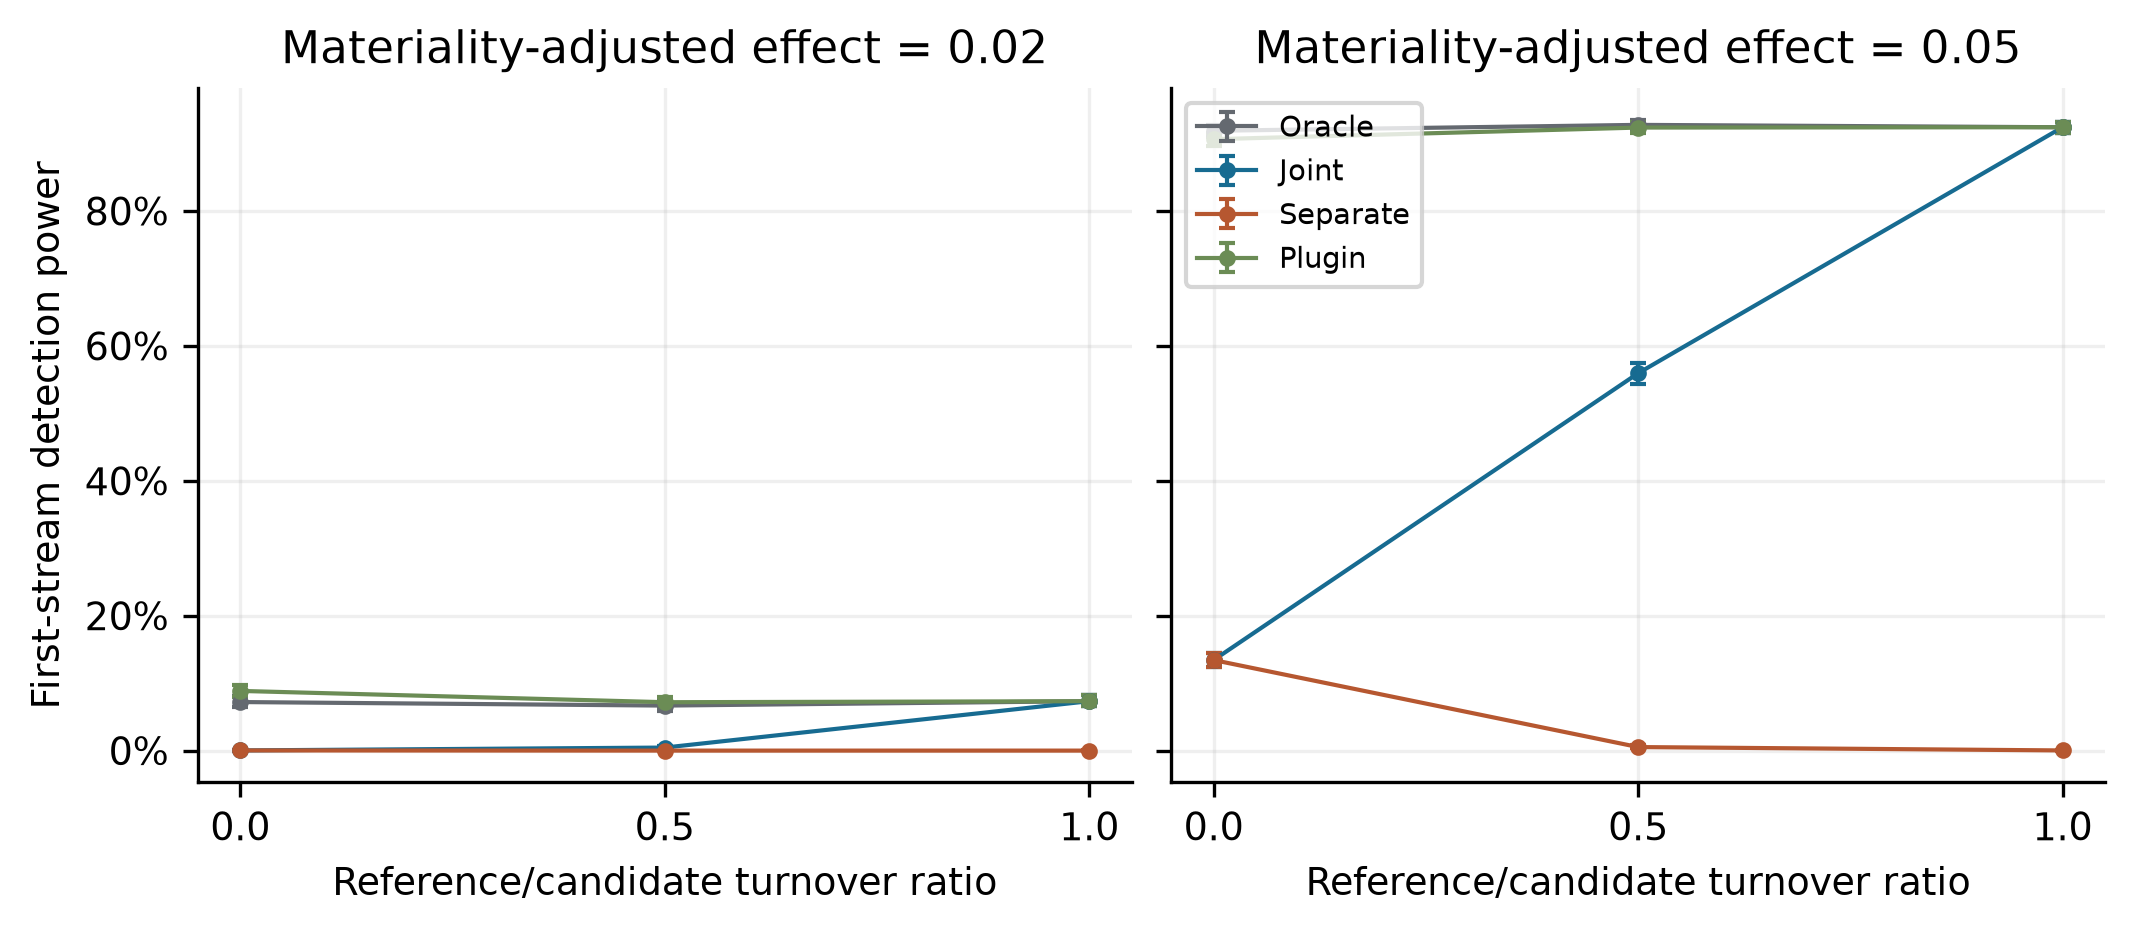
\includegraphics[width=\textwidth]{generated/simulation-power.png}
\caption{Overlap/effect comparison with 95\% Wilson intervals over independent
worlds. Methods within a case use paired data. Plugin is unguaranteed. Lines
connect three evaluated points; overlap cases use separate seeds.}\label{fig:power}
\end{figure}

The invalid symmetric-upper rule gives \UpperBothFWER\% false family rejection
[\UpperNullLower\%, \UpperNullUpper\%] when the reference trades more
(Figure~\ref{fig:validity}). A conservative cost convention for each portfolio
is therefore not necessarily conservative for their difference. Under the
explicitly invalid cost-shift law, every world's envelope eventually fails
and plugin false rejection is \PluginDriftFWER\%
[\PluginDriftLower\%, \PluginDriftUpper\%]. Low joint rejection in that
particular violation case does not restore its missing stationarity guarantee.

All four Hoeffding, fixed-time and peeked controls have zero rejections in every
case. Their support bound and the chosen signal/noise scale are too conservative
to provide an informative empirical optional-stopping comparison. These results
do not demonstrate peeking inflation, and absence of observed inflation does
not validate peeking. Appendix~\ref{app:counterexamples} addresses separate
invalidity mechanisms exactly, without substituting a favorable new simulation.

\begin{figure}[tbp]\centering
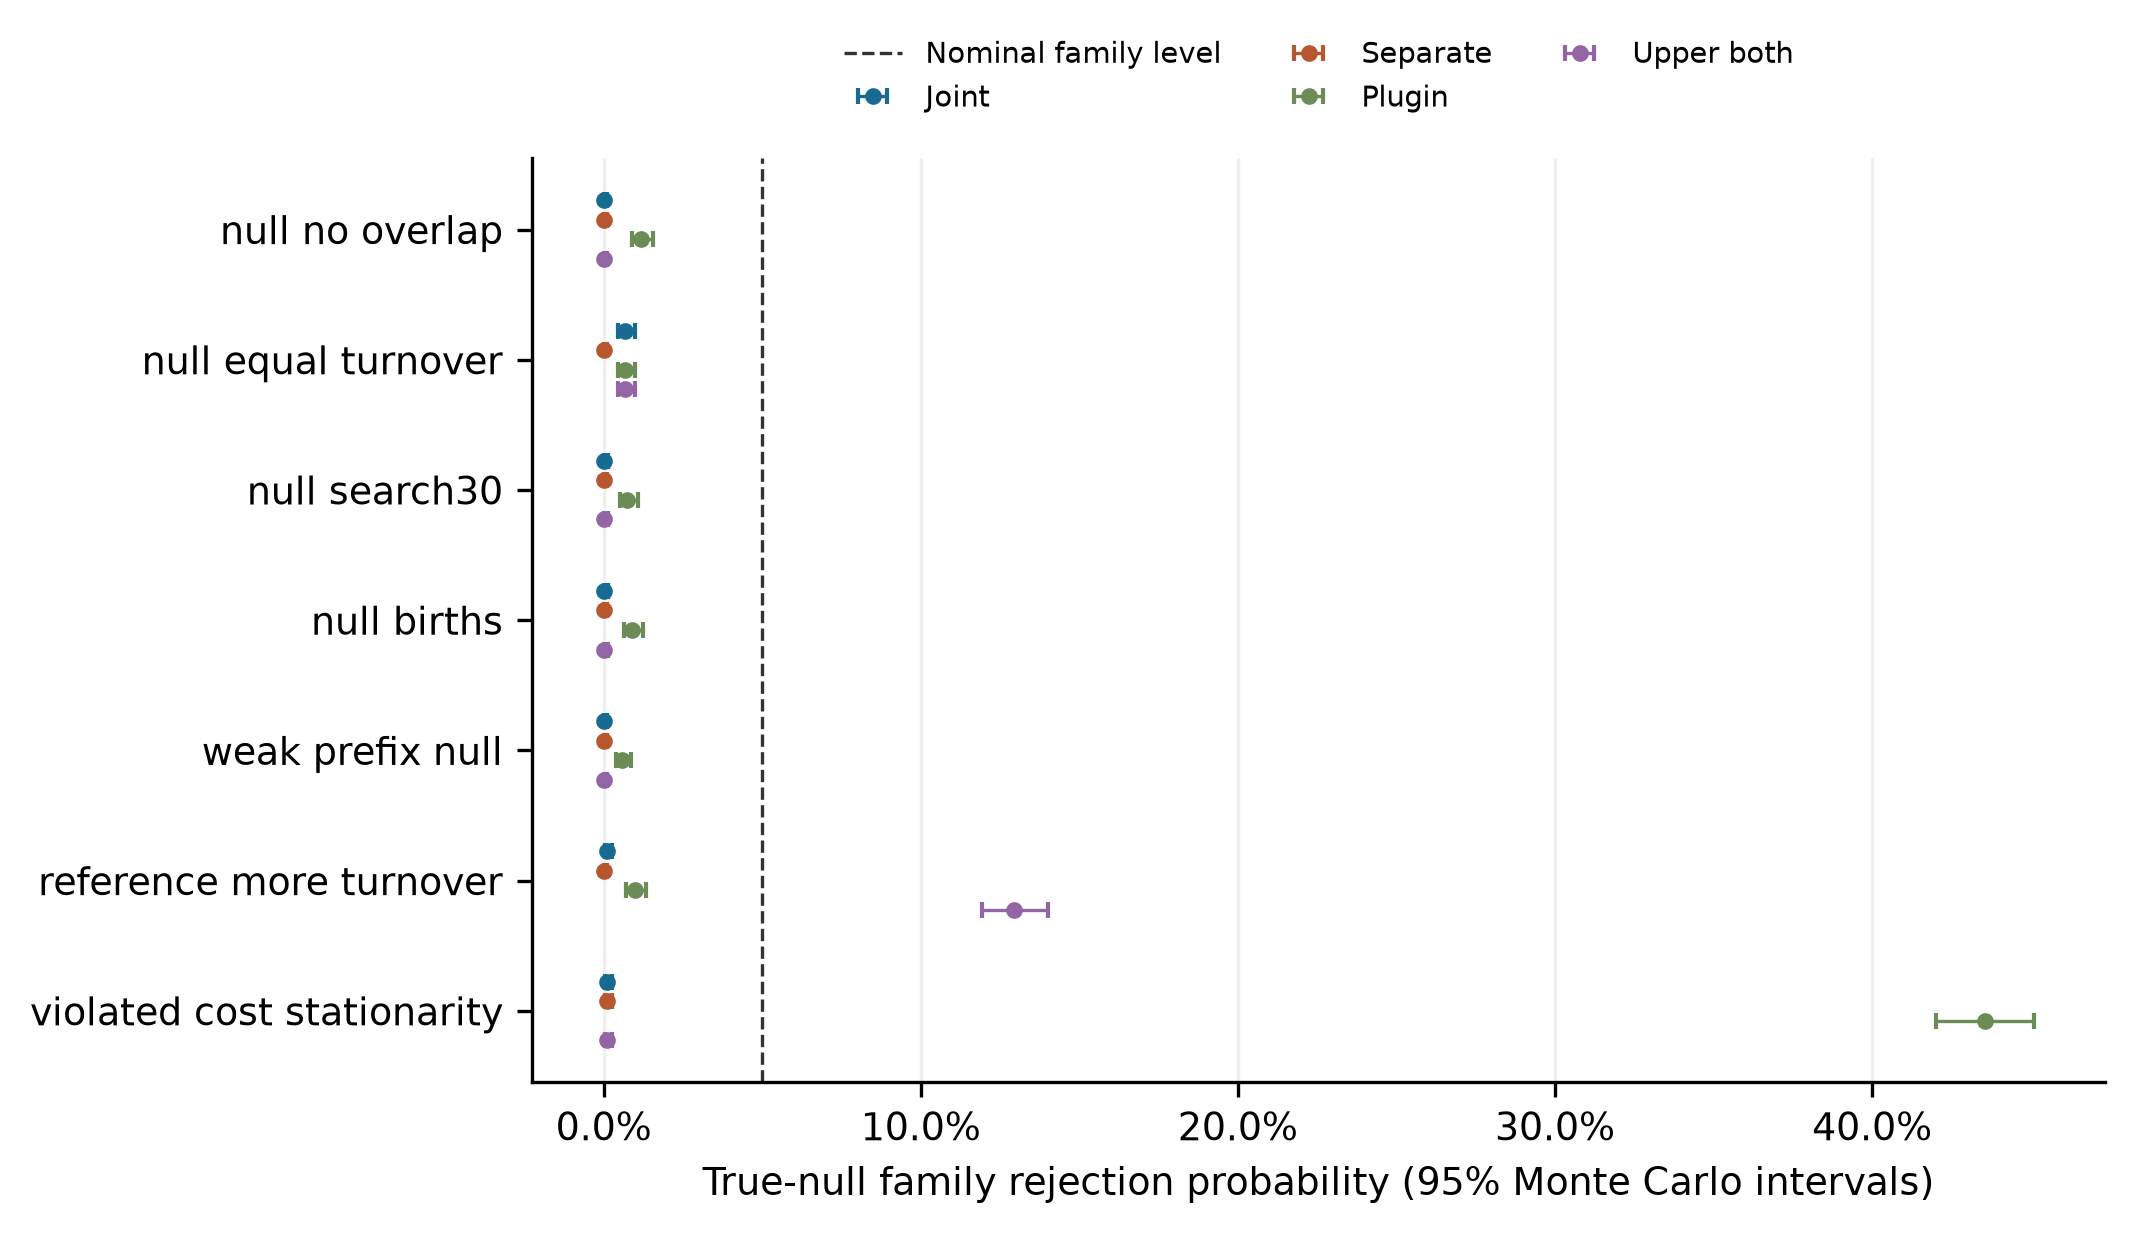
\includegraphics[width=\textwidth]{generated/simulation-validity.png}
\caption{Selected null diagnostics; the supplement retains every method/case.
The final row violates stationary calibration. Upper both and Plugin have no
asserted guarantee. Zero estimates retain nonzero Wilson upper bounds. The
dashed line is the declared 5\% family level.}\label{fig:validity}
\end{figure}

\subsection{Timing, utility and computation}

Equal-turnover joint restricted first-alternative detection time is 298.3
calendar steps versus 799.9 for separate bounds. The paired mean paper-utility
difference is 24.946 synthetic units [24.650,25.242], an approximate normal
Monte Carlo interval. This reflects the registered allocation rule and effect,
not dollars, compounded wealth, actual execution quality or general optimality
(Figure~\ref{fig:utility}).

Delay reduces matured labels from 800 to 160 and calibration opportunities,
so the lower power does not isolate delay alone. Birth cases change the family
from ten streams to five, give the first birth a larger allowance (0.02 versus
0.004), and stagger observation counts. Higher first-stream power cannot be
attributed solely to adaptation or prescreening. Within-case joint/separate
contrasts remain paired.

Case runtimes sum to 2,715.6 seconds with concurrent local work; this is a
recorded-host observation, not a controlled speed benchmark. Mixture-array
bytes are reported separately from whole-process peak memory, which was not
measured. Saved worlds support independent truth-mask, crossing-time, summary
and activation checks. Per-trial latent trajectories require the frozen
generator and seed; they are not stored in the final world arrays.

\begin{figure}[tbp]\centering
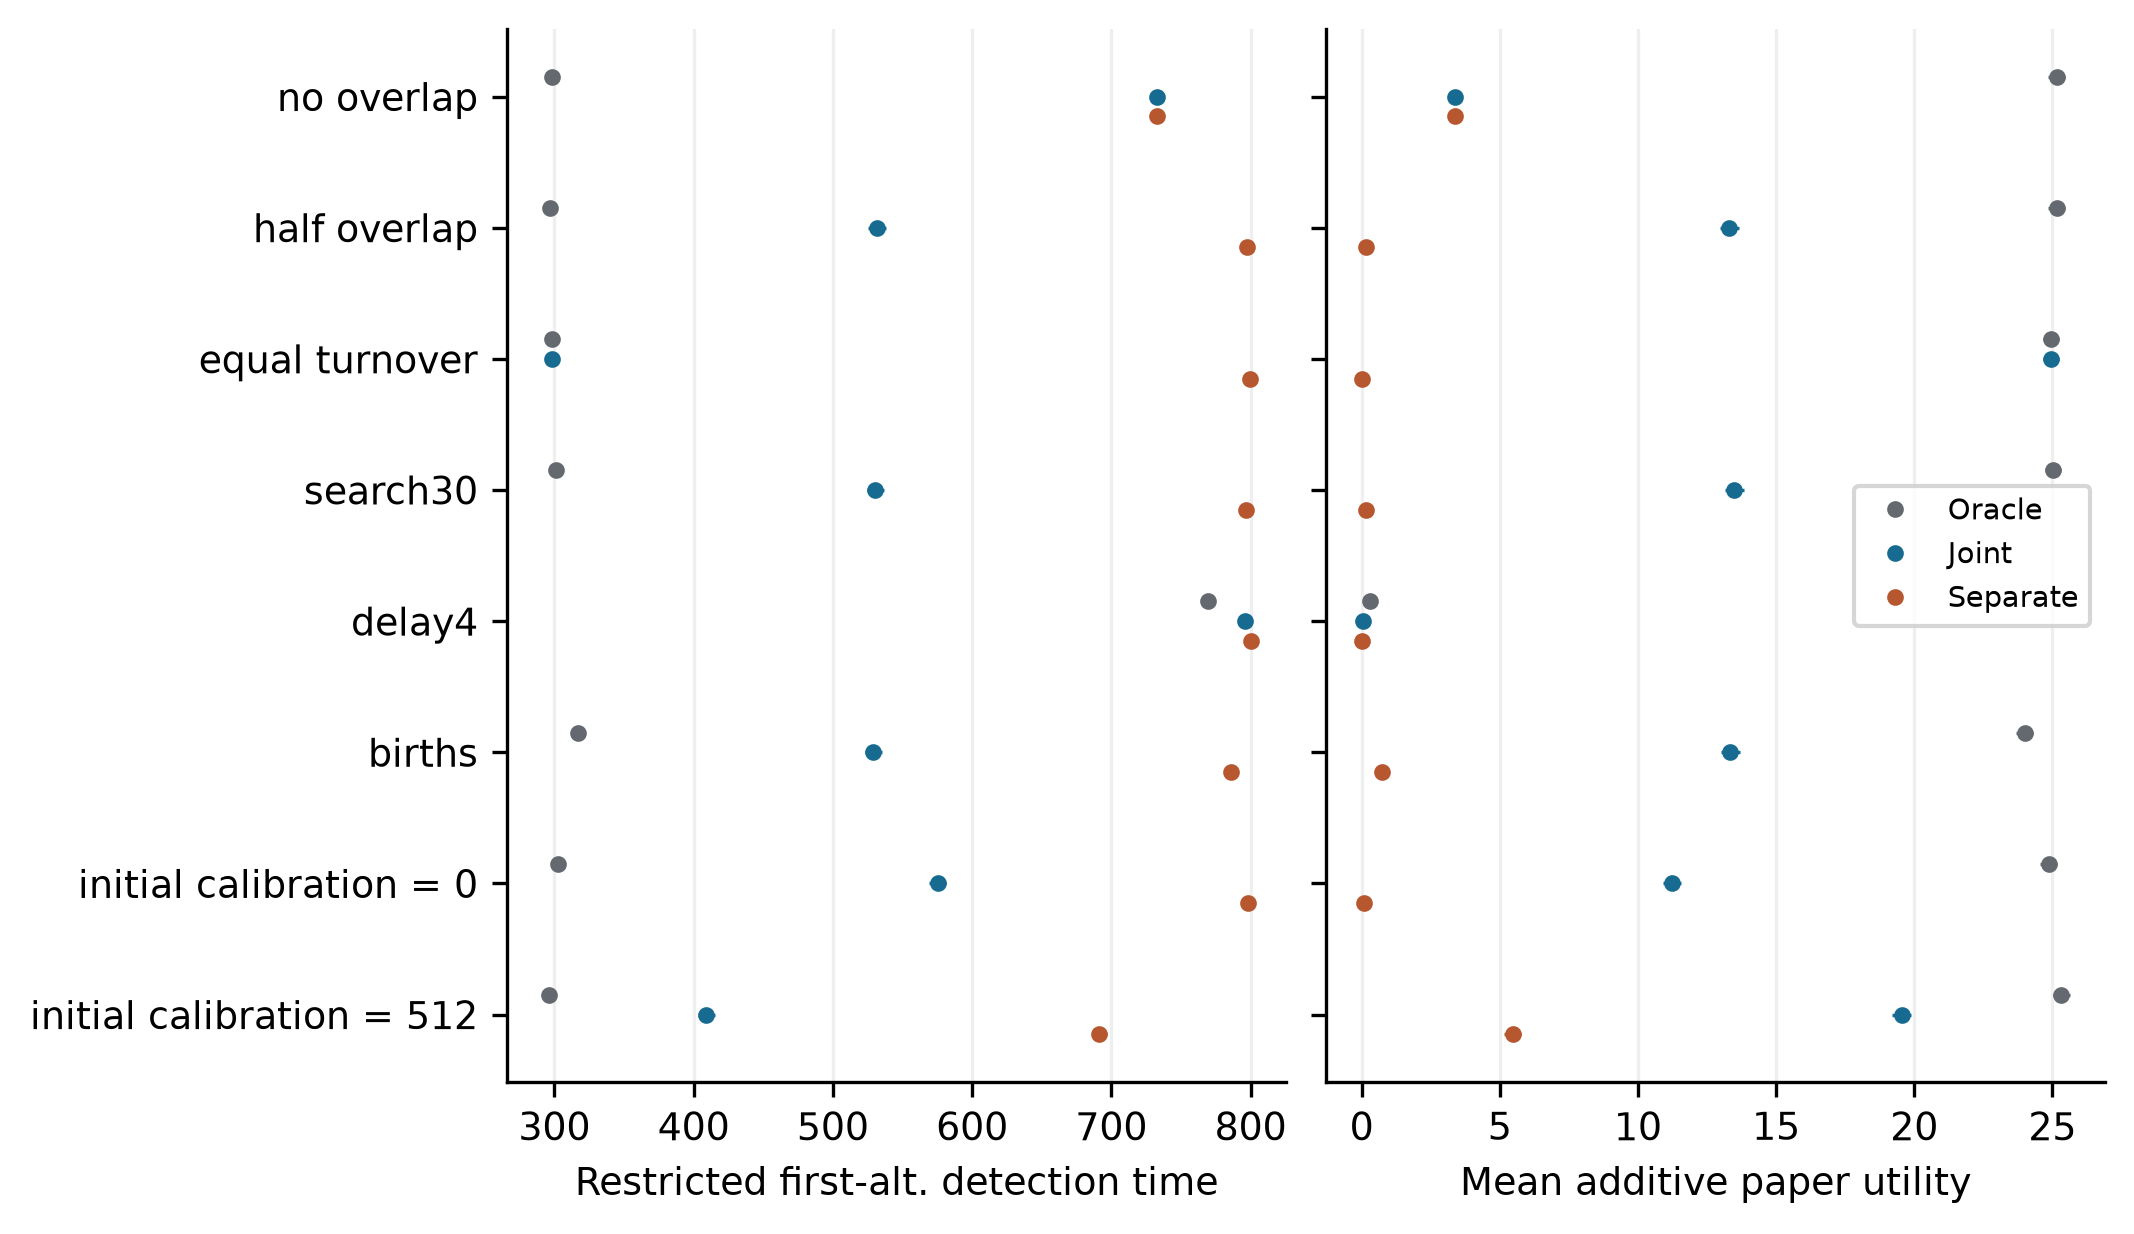
\includegraphics[width=\textwidth]{generated/simulation-delay-utility.png}
\caption{Effect-0.05 diagnostics. Time is first any-alternative discovery from
origin, horizon-censored; Figure~\ref{fig:power} reports first-stream power.
Approximate Monte Carlo intervals are omitted for degenerate samples.
Between-case comparisons change several design factors.}\label{fig:utility}
\end{figure}

\subsection{Separating evidence form from temporal cost pessimism}
\label{sec:followup-results}

All 25 separately frozen follow-up cases completed at 4,000 worlds and 800
labels. Across method/case combinations within their stated null scope, the
largest observed true-null family rejection rate is
\FollowupSupportedMaxNullRate\%. No used cost-envelope failure or interval
conflict was observed. These frequencies support the implementation checks;
they do not establish sharpness of the nominal 5\% bound. The calibration
spending rule is deliberately conservative, and neither cases nor comparators
constitute one jointly controlled family of research conclusions.

Figure~\ref{fig:followup-power} displays all eight prespecified effect-0.05
factorial cells. With high volatility, fixed cost information and alternating
turnover differences, coherent EB has \FollowupStaticAltCoherent\% first-stream
power versus \FollowupStaticAltLocal\% for local joint EB. With contracting
information these become \FollowupContractAltCoherent\% and
\FollowupContractAltLocal\%. The paired contrasts in
Table~\ref{tab:followup-paired} retain their Monte Carlo uncertainty. In the
low-volatility fixed/alternating cell, the coherent/local difference reaches
\FollowupCoherentGainMax\ percentage points. Thus a local robust calculation
can discard much of the available evidence even when its per-label cost
geometry is correct. The static, one-sign controls show zero observed
coherent/local gain. This is an observed property of these controls, not a
general EB equality: the adverse endpoint of a nonmonotone factor can change
across labels.

\begin{figure}[tbp]\centering
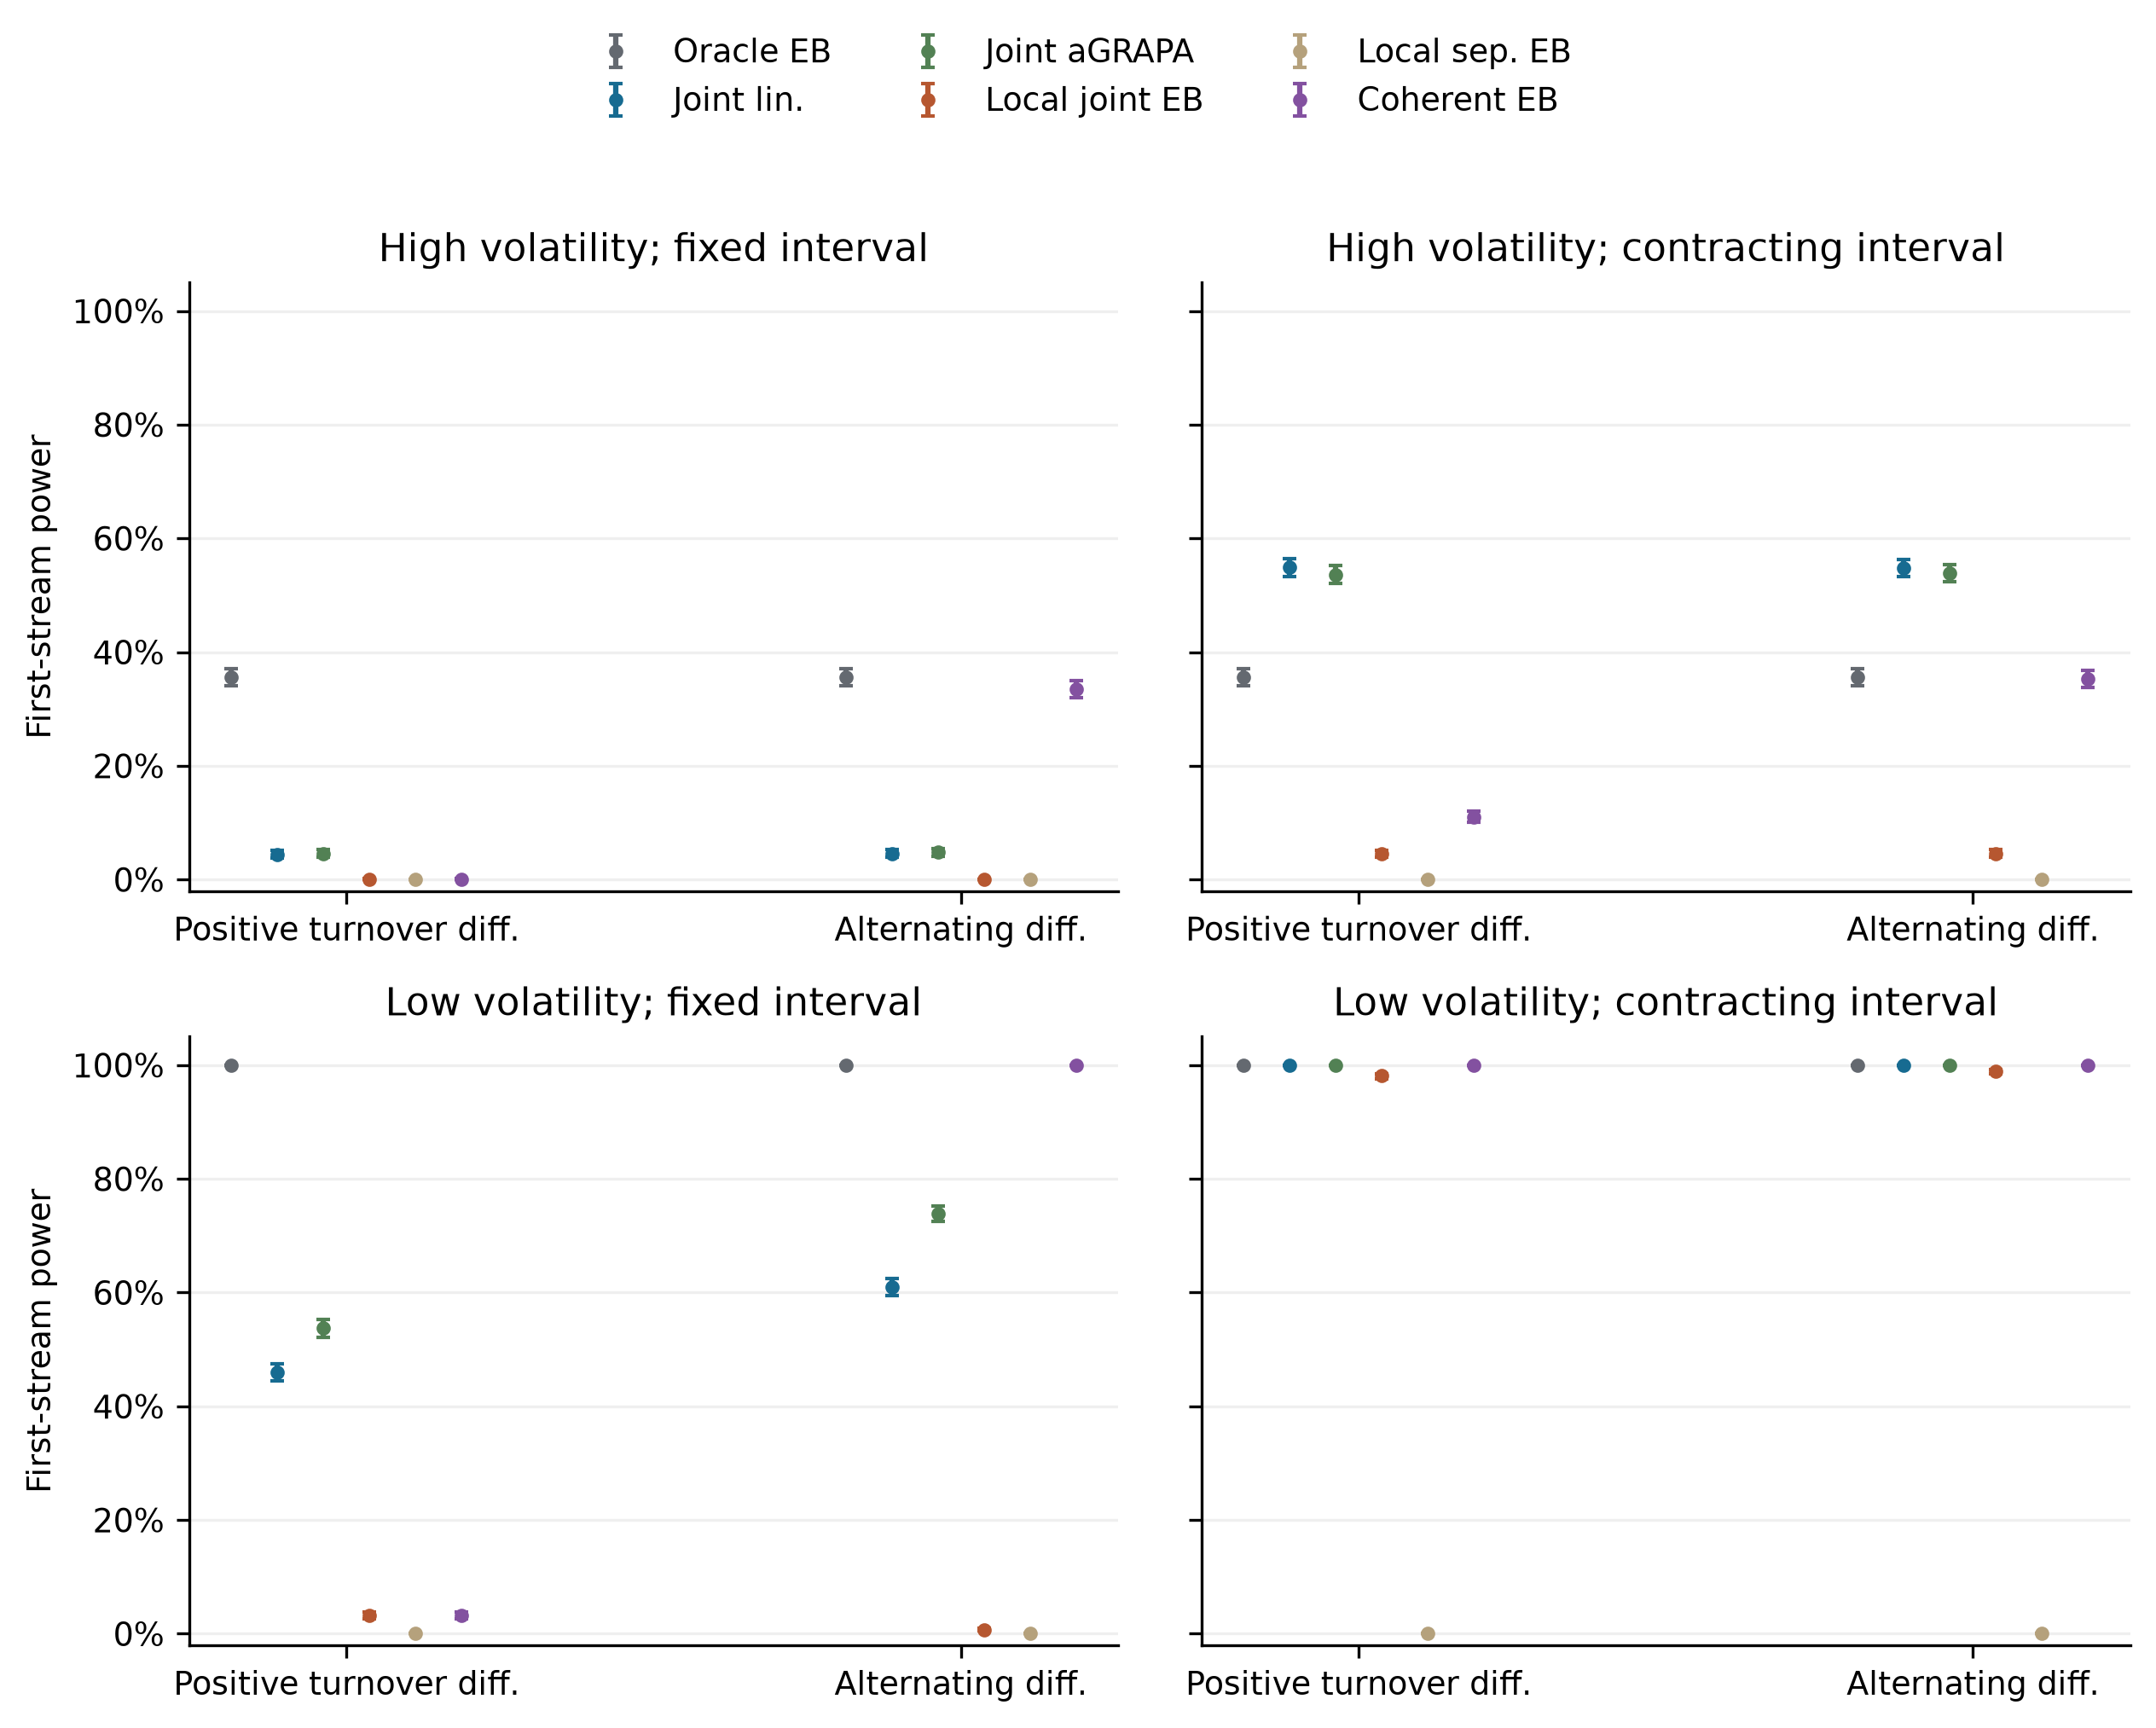
\includegraphics[width=\textwidth]{generated/followup/power.png}
\caption{Follow-up effect-0.05 factorial comparison. Points have within-case
95\% Wilson intervals over 4,000 worlds. Oracle EB knows the true cost;
its predictable centers match the other EB methods. Static and contracting
information use different calibration schedules. Factorial cells share seeded
innovations and must not be pooled as independent replications.}
\label{fig:followup-power}
\end{figure}

Temporal coherence does not make EB uniformly preferable to other evidence
forms. Under high volatility and contracting information, joint linear betting
has greater power than coherent EB, for both turnover patterns. Lower volatility
and sign changes can reverse that comparison. Likewise, the joint aGRAPA minus
joint linear power contrast ranges from \FollowupAgraGainMin\ to
\FollowupAgraGainMax\ percentage points across the eight primary cells. Its
negative high-volatility/contracting contrasts and positive low-volatility/static
contrasts rule out a uniform empirical advantage. Predictable refitting also
has a stronger conditional-null requirement than the fixed-grid comparisons.

Local joint versus local separate EB gains range from
\FollowupJointSeparateGainMin\ to \FollowupJointSeparateGainMax\ percentage
points. These are a different ablation from coherent versus local joint EB.
Both must be held separate from changing the underlying betting rule or the
cost-calibration schedule. The results identify mechanisms within the declared
synthetic family, rather than a universally best sequential procedure.

Weak effects remain difficult. Across the eight effect-0.02 cells, coherent EB
first-stream rejection never exceeds 1.825\%. The stronger effect-0.05 gains
therefore do not establish sensitive detection of small improvements at this
horizon, even inside the synthetic family.

\begin{table}[tb]\centering
\begingroup\small\setlength{\tabcolsep}{3pt}
\begin{tabular}{lrrr}\toprule
Case & aGRAPA - linear & Coherent - local EB & Joint - separate EB\\\midrule
F03 & 0.12 [-0.20, 0.45] & 0.00 $^{\ddagger}$ & 0.03 [-0.02, 0.07]\\
F06 & 0.18 [-0.15, 0.50] & 33.50 [32.04, 34.96] & 0.00 $^{\ddagger}$\\
F09 & -1.23 [-1.85, -0.60] & 6.48 [5.71, 7.24] & 4.50 [3.86, 5.14]\\
F12 & -0.88 [-1.50, -0.25] & 30.73 [29.30, 32.15] & 4.60 [3.95, 5.25]\\
F15 & 7.72 [6.90, 8.55] & 0.00 $^{\ddagger}$ & 3.20 [2.65, 3.75]\\
F18 & 12.90 [11.86, 13.94] & 99.30 [99.04, 99.56] & 0.70 [0.44, 0.96]\\
F21 & 0.00 $^{\ddagger}$ & 1.90 [1.48, 2.32] & 98.10 [97.68, 98.52]\\
F24 & 0.00 $^{\ddagger}$ & 1.10 [0.78, 1.42] & 98.90 [98.58, 99.22]\\
\bottomrule\end{tabular}
\endgroup
\caption{Prespecified effect-0.05 contrasts in first-stream power, in percentage points. Intervals are paired, approximate, unadjusted 95\% normal Monte Carlo intervals across worlds. $^{\ddagger}$ marks a degenerate sample with an unavailable normal interval, not known zero uncertainty. Case definitions appear in the supplement.}\label{tab:followup-paired}
\end{table}


\begin{figure}[tbp]\centering
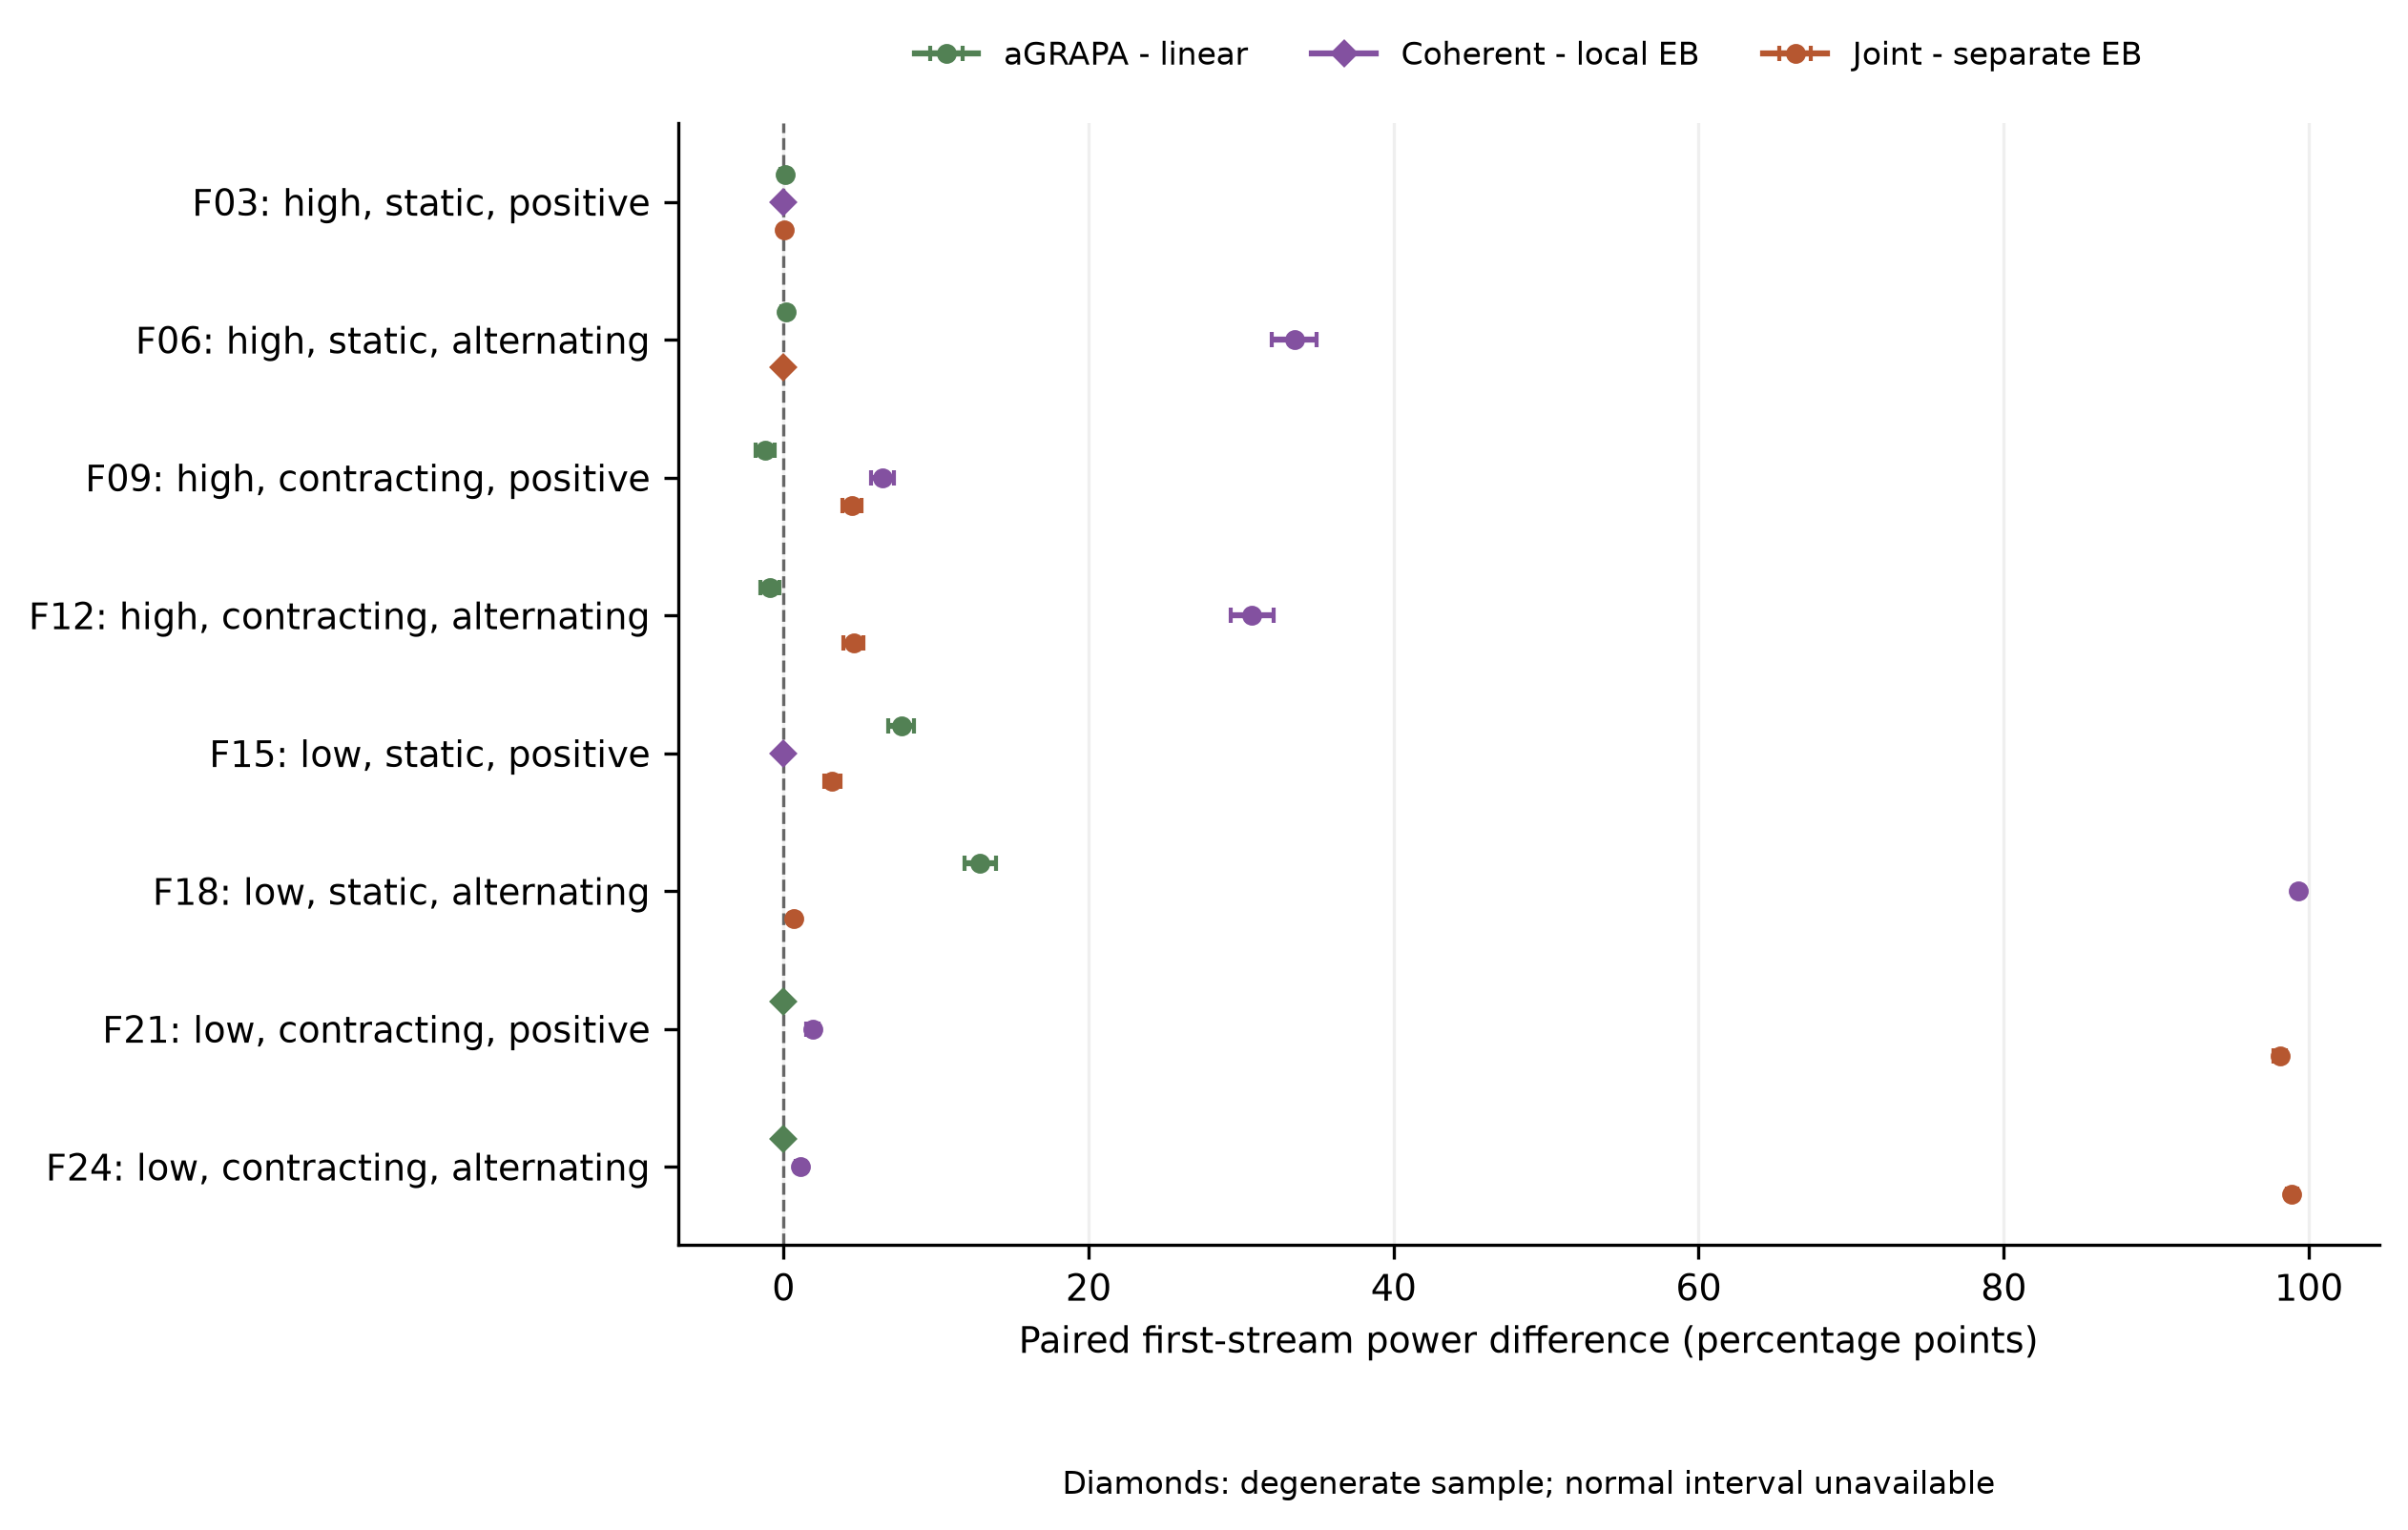
\includegraphics[width=\textwidth]{generated/followup/paired-power.png}
\caption{The three primary within-case ablations, with paired approximate
95\% normal Monte Carlo intervals. Intervals are unadjusted descriptive
summaries; diamonds denote degenerate samples for which that normal interval
is unavailable. Every registered contrast, including weaker effects, is
retained in the machine-readable supplement.}
\label{fig:followup-paired}
\end{figure}

Restricted detection time and subsequent paper utility follow the same
implementation's recorded allocation rule, not a funded portfolio. Saturated
end-of-horizon power does not imply identical detection times or utility;
those endpoints remain in the complete result tables. The prefix-weak diagnostic
has no first-stream rejections for any method. Its family rejection counts are
one for oracle linear, two for oracle aGRAPA and zero for the other methods,
out of 4,000 worlds each. These low frequencies do not validate aGRAPA
under that weaker null: Section~\ref{sec:followup-methods} gives its scope and
a deterministic counterexample to general predictable refitting.

Case kernels total 2,542.6 seconds on the recorded host. Named persistent state
uses 24,220,080 bytes per case; this is not peak process memory and runtime
excludes serialization. These observations describe reproducibility costs,
not controlled speed comparisons. All 250 method summaries, 150 paired
contrasts, calibration diagnostics and source-linked array outputs are retained.


\subsection{No demonstrated adaptive Bitcoin edge}

The primary four-hour period has 3,948 scored candles, no missing scored
intervals and no feature pauses. The selector makes no switches. Its full
Binance history has 27 decisions, all retaining EMA 50/200. Fixed/adaptive raw
paths are exactly identical, with the same \PrimaryFixedReturn\% primary
return (Table~\ref{tab:market}). The ensemble returns \PrimaryEnsembleReturn\%.
These point estimates do not establish adjusted superiority over the controls.

\begin{table}[tbp]\centering\small
\begin{tabular}{lrrrrr}\toprule Policy & Return (\%) & Max DD (\%) & Exposure (\%) & Trades & Turnover\\\midrule
Fixed EMA 50/200 & 2.61 & -20.05 & 26.8 & 31 & 13.54\\
Adaptive & 2.61 & -20.05 & 26.8 & 31 & 13.54\\
Ensemble & -2.21 & -20.09 & 25.7 & 88 & 14.68\\
Cash & 0.00 & 0.00 & 0.0 & 0 & 0.00\\
Buy and hold & -11.27 & -53.45 & 100.0 & 0 & 0.00\\
Volatility target & -6.30 & -36.73 & 51.5 & 20 & 2.26\\
Slow resizing & 4.84 & -18.50 & 26.3 & 27 & 12.75\\
Fixed EMA 25/100 & -5.17 & -22.65 & 24.4 & 57 & 25.51\\
Fixed EMA 100/400 & -4.63 & -21.26 & 26.8 & 17 & 6.65\\
\bottomrule\end{tabular}

\caption{Primary retrospective four-hour policies at 25 bps per side. Exposure
is average closing weight; turnover sums absolute traded notional divided by
pre-trade wealth. Holdings are inherited and terminal holdings marked.}
\label{tab:market}
\end{table}

Bitstamp has two pre-window switches and different inherited wealth, but no
scored-window switches. Its rebased paths agree to floating-point precision.
Differences around $10^{-16}$ produce some raw cost-grid sign changes; these
are not economic break-even costs. A post-outcome note preserves raw artifacts
and marks per-bar differences within $10^{-12}$ as numerical identity.
Binance's zero bootstrap interval and Bitstamp's roundoff intervals resample
an identical historical difference, not a known zero future advantage.

\begin{figure}[tbp]\centering
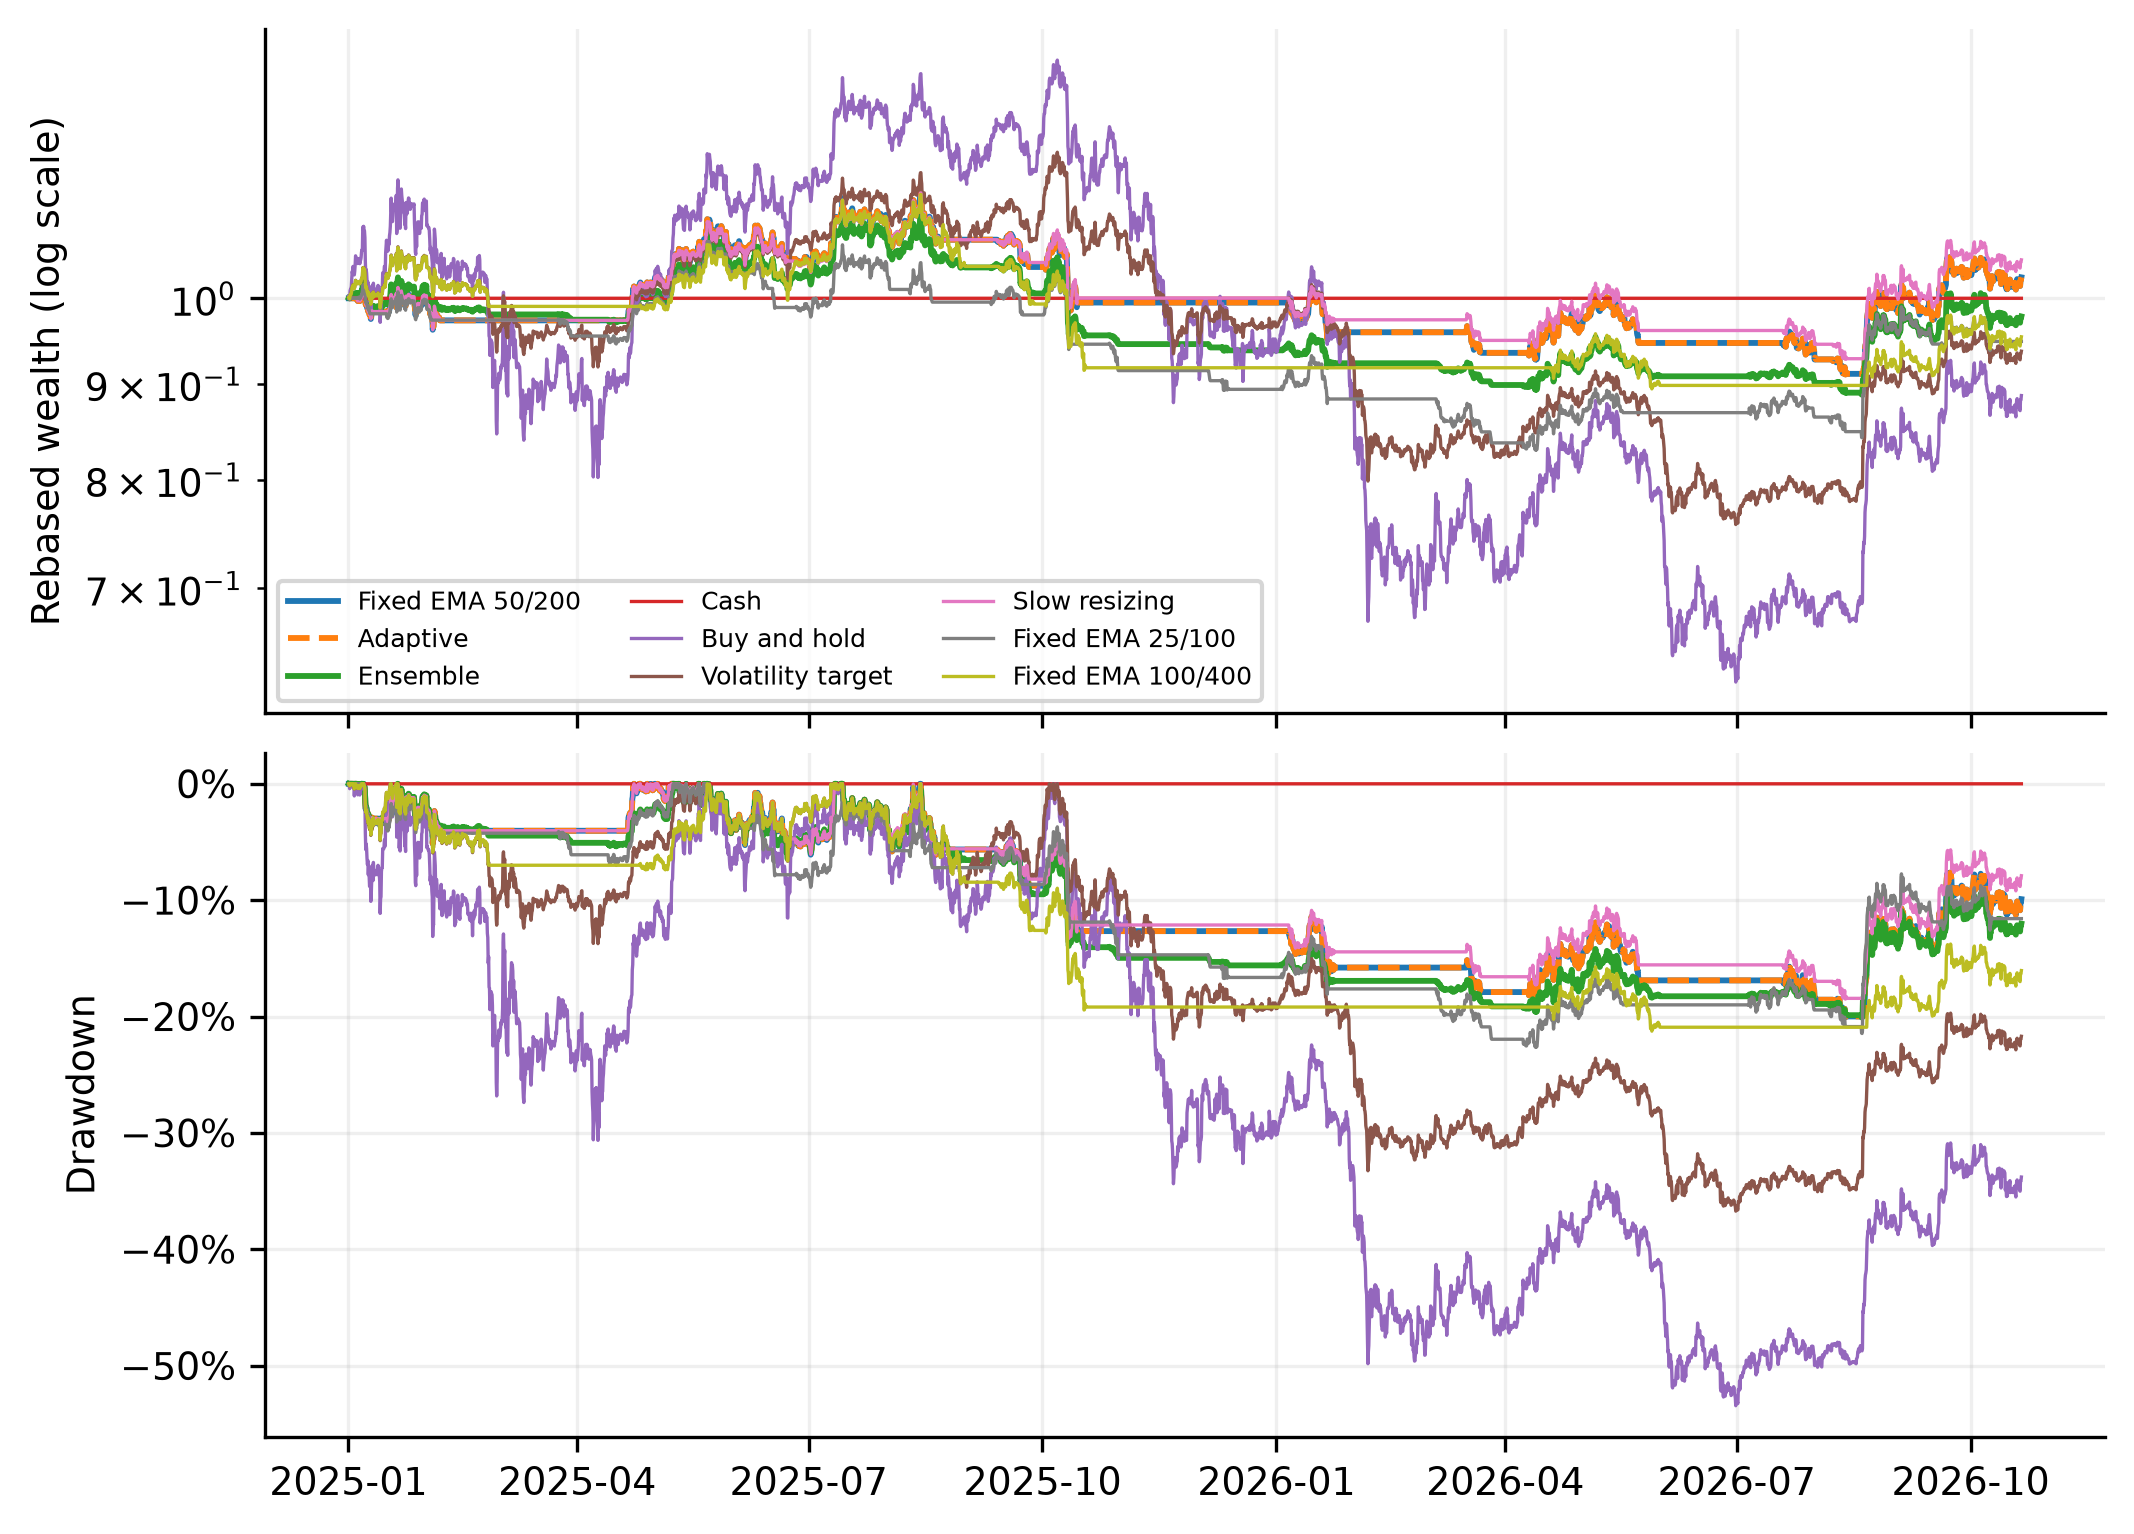
\includegraphics[width=\textwidth]{generated/market-primary-paths.png}
\caption{Primary rebased wealth and drawdown at assumed 25 bps. Adaptive and
fixed lines coincide. Passive and risk-controlled books have different
exposures; no line represents verified historical fills.}\label{fig:marketpaths}
\end{figure}

On the common 243-day window, hourly and daily adaptive annualized mean-log
differences are $-9.653\%$ and $-6.681\%$ at base cost. The hourly approximate
30-day interval is $[-32.175\%,2.610\%]$; the daily interval is
$[-22.419\%,5.042\%]$.
Both span losses and gains, including the 2\% materiality threshold. Neither
material gain nor stable loss is established. There are two hourly and three
daily switches. These are dependent market observations, not independent
replications or evidence of a universally best timeframe.

There are only 8.1 nominal 30-day blocks in this 243-day window. This does not
validate stability or finite-sample coverage. A post-outcome deterministic
diagnostic in Table~\ref{tab:blockedges} shows the finite-sample edge weighting
of the specified non-circular resampler: its expected resampled mean differs
from the observed mean. These are not new intervals, and no better-looking
correction replaces the registered percentile results.

\begin{table}[tbp]\centering\small
\begin{tabular}{lrrr}
\toprule
Case & Nominal blocks & Observed & Expected resample\\
\midrule
Hourly & 8.1 & -9.653\% & -11.150\%\\
Daily & 8.1 & -6.681\% & -7.256\%\\
\bottomrule
\end{tabular}

\caption{Primary 25 bps matched-window mean log differences, annualized linearly.
The expected resample averages exactly over all possible block starts, including
the final truncated block. Nominal block count is not an independent sample size.}
\label{tab:blockedges}
\end{table}

All five costs leave four-hour comparisons identical and hourly/daily point
estimates negative. Neither nonidentical case has a cost-grid sign-change
bracket. The hourly deficit shrinks slightly at larger costs, illustrating why
reference costs must enter the paired contrast. Direct fee-drag differences
are small relative to the hourly/daily price/holdings differences; this is
accounting description, not causal attribution. All cost/control outcomes are
retained in the supplement.

\begin{table}[tbp]\centering\small
\begin{tabular}{lrrr}\toprule Case & Annual log diff. (\%) & 30-day interval (\%) & Switches\\\midrule
Binance primary 4h & 0.00$^\dagger$ & identical path$^\dagger$ & 0\\
Binance matched 4h & 0.00$^\dagger$ & identical path$^\dagger$ & 0\\
Binance matched 1h & -9.65 & [-32.18, 2.61] & 2\\
Binance matched 1d & -6.68 & [-22.42, 5.04] & 3\\
Bitstamp primary 4h & 0.00$^\dagger$ & identical path$^\dagger$ & 0\\
Bitstamp matched 4h & 0.00$^\dagger$ & identical path$^\dagger$ & 0\\
\bottomrule\end{tabular}

\caption{Base-cost paired results. $\dagger$ denotes historical numerical
identity, not zero future uncertainty. Other intervals are approximate,
retrospective and unadjusted.}\label{tab:pairedmarket}
\end{table}

\begin{figure}[tbp]\centering
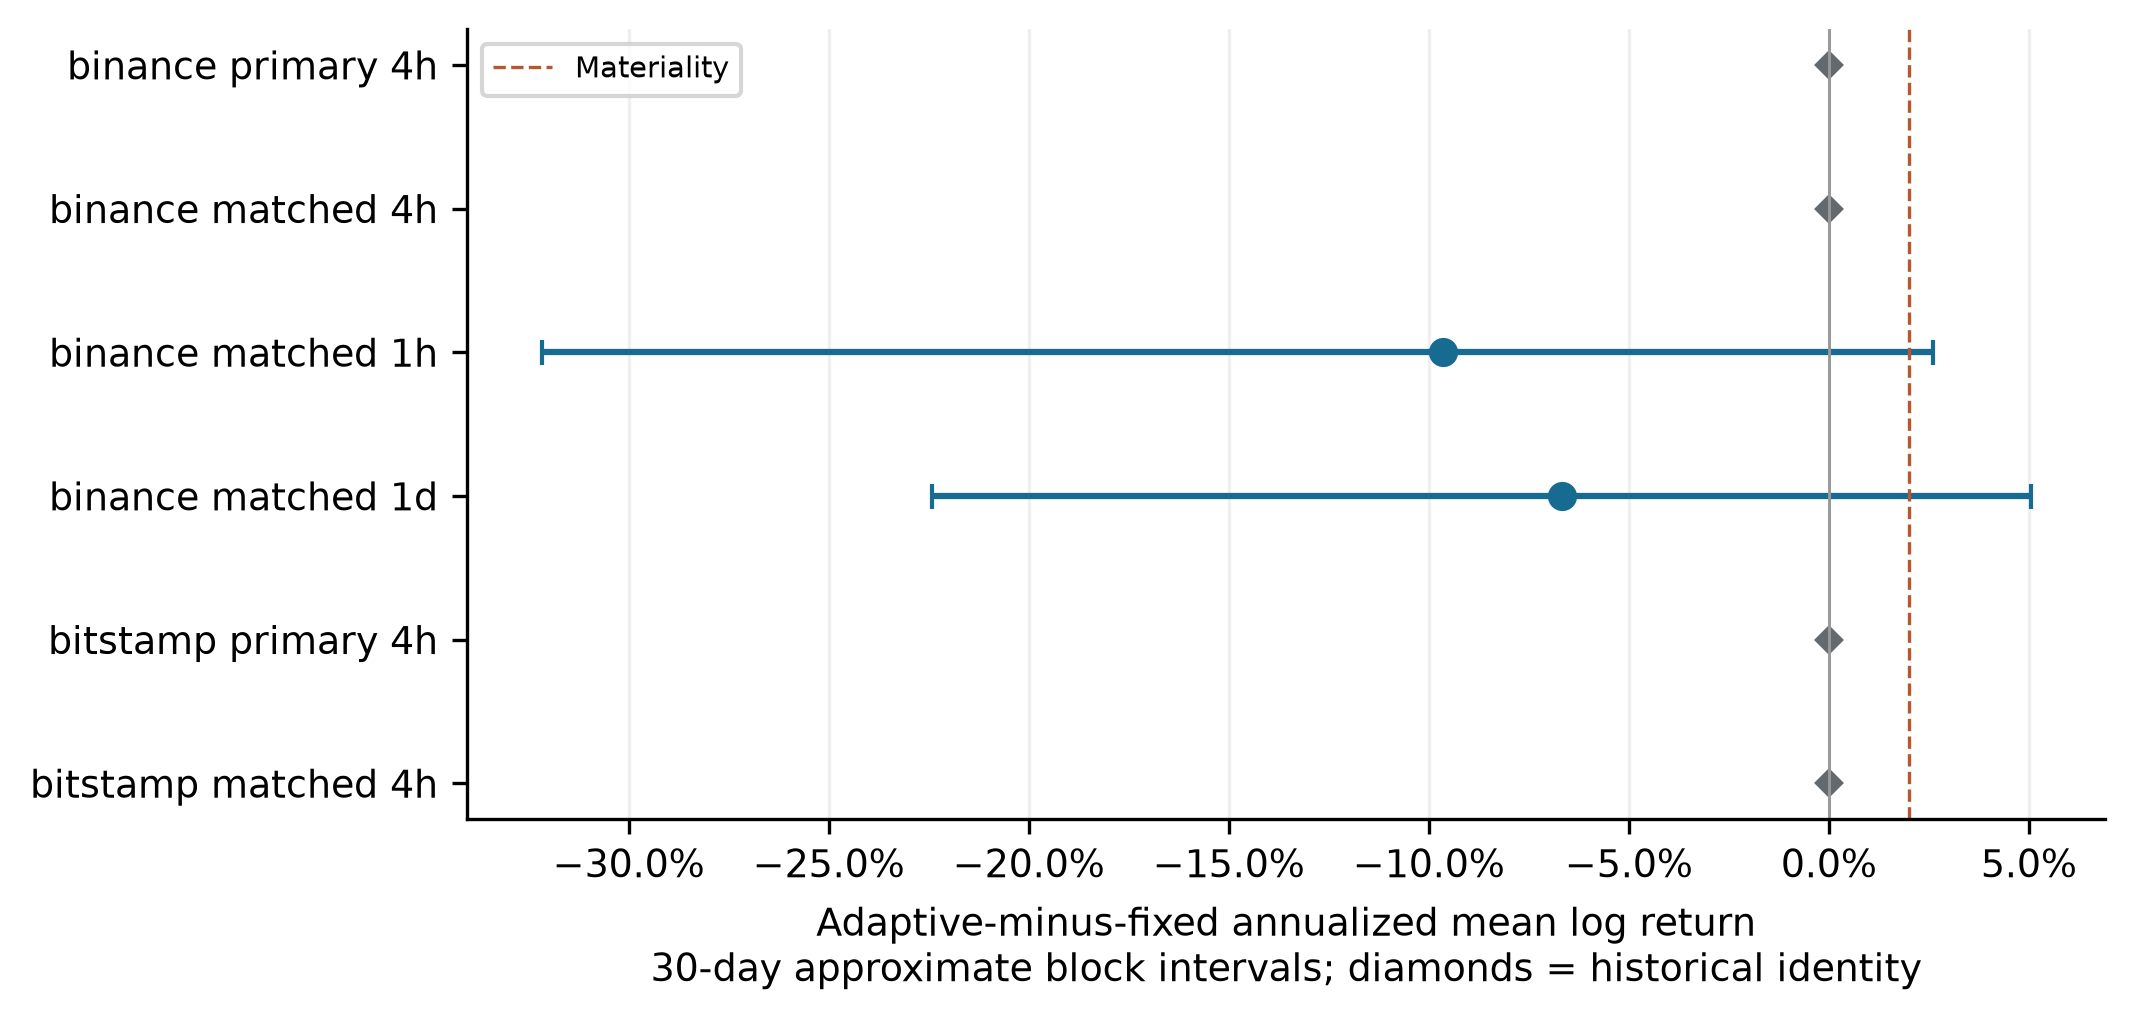
\includegraphics[width=\textwidth]{generated/market-paired-intervals.png}
\caption{All six prespecified application cases. Diamonds mark historical
identity. Intervals are not sequential or research-selection-adjusted evidence.
The dashed line is annual log materiality 0.02.}\label{fig:pairedmarket}
\end{figure}

\section{Interpretation, limitations and reproducibility}

Sequential error control, historical economic performance and execution
feasibility answer different questions. Cost calibration assumptions are
substantive restrictions, not facts supplied by OHLCV data. The synthetic
construction isolates paired-cost uncertainty under known truth; it cannot
validate a common stationary market cost parameter, nor show that selected
Bitcoin strategies satisfy a bounded conditional null.

Likewise, a confidence interval from one retrospective price history does not
create additional independent markets. Native candle frequencies differ in
outage history as well as discretization, and a strict reset policy sacrifices
history to avoid manufacturing tradable bars. USD and USDT quote risks remain
unmodeled. No capacity or actual fill inference is supported by these inputs.
Zero interest on cash is a modeling choice that changes relative performance.

The practical result is a negative one for the tested four-hour EMA selector: the primary
procedure never departs from its reference, and the nonidentical timeframe
checks do not establish material improvement. The synthetic power advantage
depends on a defensible shared cost coefficient. It is not evidence that this
cost structure has been calibrated for the Bitcoin application. Improving
the statistical comparison and improving the trading rule are distinct tasks.

The novelty claim is limited to the completed diagnostic findings and their
auditable connection to the application. The underlying bounded betting,
coverage composition and robust-cost identities are established. The follow-up
shows that local cost pessimism, temporal information loss and evidence-form
choice have different empirical consequences. Its matched profiling gain is
not a new composite-inference theorem. Large synthetic gains and a negative
market result can coexist because the market application does not establish
the synthetic cost assumptions. Further claims require new prespecified
experiments and nearest-work review.

The implementation uses locked Python dependencies, deterministic seeds,
synthetic accounting/leakage tests, immutable inputs, source snapshots,
configuration/runtime fingerprints and a transactional SQLite attempt ledger.
Publication and smoke runs are labeled separately. Freeze creation for the
market application checks feature coverage without evaluating portfolio P\&L.
All attempts, including failures and partial runs, are retained. A local freeze
is not an independently witnessed preregistration or a mechanism preventing
human or model prior knowledge.

\paragraph{Availability and reproducibility.}
The accompanying research distribution preserves the exact source ZIPs used by both
synthetic cohorts and the market study, specifications, protocols, hashes,
all case outputs and full attempt-ledger snapshots. Generated displays contain
216 baseline and 250 follow-up method/case rows, 150 follow-up paired contrasts,
270 market policy/cost rows and 30 primary paired cost rows.
AI-assisted internal consistency checks recomputed world summaries, accounting,
timing, selector behavior and paired intervals. Check scopes and source
fingerprints are retained. These automated checks are not independent human
peer review or a human-author approval record. The declarations identify the
tool, its substantive roles and the limits of the recorded model information.
The documented single entry point verifies preserved evidence, rebuilds this
paper, or replays all studies from their archived sources. The completed
recorded-host replay reproduced the saved scientific arrays and numerical
reports exactly. Its combined invocation reverified an earlier full baseline
replay and freshly recomputed the follow-up; this creates no new independent
worlds or market observations. Final-paper sources are bound to a separate
completed rebuild, with rendered-page QA and local archive checks recorded
alongside the replication instructions. The submission companion separates a
LaTeX source bundle from a code/results replication bundle. Raw vendor candles
are not included in the public replication bundle. An explicit results-only
mode rebuilds displays and the manuscript without claiming a raw-data audit or
a fresh computational replay. Exact-input restoration verifies the original
hashes and reconciles normalized candles against raw records before a full
replay; revised downloads fail that check rather than being relabeled as the
original snapshot. Bibliographic access limits and historical revision risk
remain explicit. If revisions prevent recovery, the corresponding author can
be contacted about permitted access to preserved snapshots. The provider-specific
reuse exceptions are stated below.

\section{Conclusion}

Shared mean-cost structure can preserve substantial sequential detection power
in bounded paired experiments, while a superficially conservative upper-cost
shortcut can give false evidence when the reference trades more. Temporal
profiling can recover evidence discarded by local bounds, but method rankings
depend on volatility, calibration and turnover patterns. These are conditional
established-method findings, with calibration and information requirements made
explicit. The audited Bitcoin application demonstrates no
incremental four-hour adaptive performance and no sufficiently precise material
gain in its timeframe checks. The result supports disciplined validation of the
bot, not a claim that this implementation has found a profitable adaptive edge.

\section*{Declarations}

\paragraph{Author.}
Abdullah Hamza directed the research and is the corresponding author.
Responsibility for the submitted work rests with the named author.

\paragraph{AI assistance and responsibility.}
OpenAI Codex was used for literature research, experimental design, code
preparation and testing, statistical analysis, interpretation, figure generation,
manuscript drafting and revision, and reproducibility and release checks.
Exact model versions were not consistently recorded. The human author retains
responsibility for the final work. Automated checks and AI-assisted reviews are
not independent human peer review or evidence of completed human-author review.

\paragraph{Funding and competing interests.}
The author reports no external funding and no competing interests.
The study uses synthetic experiments and public exchange records, with no
human-subject or private account data.

\paragraph{Reuse rights and provider attribution.}
Original text and synthetic displays are copyright 2026 Abdullah Hamza,
licensed under \href{https://creativecommons.org/licenses/by/4.0/}{CC BY 4.0};
original software is MIT licensed. Third-party market material is excluded
from those grants. Binance-derived market figures, tables and accompanying
outputs retain Binance Vision attribution and
\href{https://creativecommons.org/licenses/by-nc-sa/4.0/}{CC BY-NC-SA 4.0}
under its dataset terms. Mixed-venue displays retain that exception.
Bitstamp-sourced records retain Bitstamp attribution and applicable provider
terms. The companion \texttt{THIRD\_PARTY.md} and
\texttt{LICENSE-PAPER.md} identify the scope; no unrestricted commercial
license to provider material is asserted.

% Generated by scripts/build_bibliography.py; edit verified JSON, not this file.
\begingroup\small\raggedright
\begin{thebibliography}{99}
\bibitem[Choe and Ramdas(2024)]{choe2024}
Yo Joong Choe and Aaditya Ramdas (2024). Comparing Sequential Forecasters. \emph{Operations Research}, 72(4):1368--1387.
\href{https://pubsonline.informs.org/doi/10.1287/opre.2021.0792}{doi:10.1287/opre.2021.0792}.
\bibitem[Arnold et al.(2026)]{arnold2026}
Sebastian Arnold, Georgios Gavrilopoulos, Benedikt Schulz and Johanna Ziegel (2026). Sequential model confidence sets. \emph{Journal of the Royal Statistical Society Series B: Statistical Methodology}.
\href{https://doi.org/10.1093/jrsssb/qkag066}{doi:10.1093/jrsssb/qkag066}.
\bibitem[Waudby-Smith and Ramdas(2024)]{waudby2024}
Ian Waudby-Smith and Aaditya Ramdas (2024). Estimating means of bounded random variables by betting. \emph{Journal of the Royal Statistical Society Series B: Statistical Methodology}, 86(1):1--27.
\href{https://doi.org/10.1093/jrsssb/qkad009}{doi:10.1093/jrsssb/qkad009}.
\bibitem[Howard et al.(2021)]{howard2021}
Steven R. Howard, Aaditya Ramdas, Jon McAuliffe and Jasjeet Sekhon (2021). Time-uniform, nonparametric, nonasymptotic confidence sequences. \emph{The Annals of Statistics}, 49(2):1055--1080.
\href{https://doi.org/10.1214/20-AOS1991}{doi:10.1214/20-AOS1991}.
\bibitem[Xu and Ramdas(2024)]{xu2024}
Ziyu Xu and Aaditya Ramdas (2024). Online multiple testing with e-values. \emph{Proceedings of the 27th International Conference on Artificial Intelligence and Statistics, PMLR}, 238:3997--4005.
\href{https://proceedings.mlr.press/v238/xu24a.html}{Source and version}.
\bibitem[Tian and Ramdas(2021)]{tian2021}
Jinjin Tian and Aaditya Ramdas (2021). Online control of the familywise error rate. \emph{Statistical Methods in Medical Research}, 30(4):976--993.
\href{https://doi.org/10.1177/0962280220983381}{doi:10.1177/0962280220983381}.
\bibitem[Jiao et al.(2026)]{jiao2026}
Zhanyi Jiao, Qiuqi Wang and Yimiao Zhao (2026). Comparative e-backtests for general risk measures. \emph{arXiv preprint}, arXiv:2511.05840v2.
\href{https://arxiv.org/abs/2511.05840v2}{Source and version}.
\bibitem[Liu(2026)]{liu2026}
Xiaoquan Liu (2026). Anytime-Valid Tests of Factor Alphas. \emph{SSRN working paper}.
\href{https://papers.ssrn.com/sol3/papers.cfm?abstract_id=7357270}{doi:10.2139/ssrn.7357270}.
Working paper; only indexed abstract inspected.
\bibitem[Stephan(2026)]{stephan2026}
Rany Stephan (2026). Sequential Tradeability Testing for Alpha Signals. \emph{SSRN working paper}.
\href{https://ssrn.com/abstract=6922558}{doi:10.2139/ssrn.6922558}.
Working paper; only indexed abstract inspected.
\bibitem[Wasserman et al.(2020)]{wasserman2020}
Larry Wasserman, Aaditya Ramdas and Sivaraman Balakrishnan (2020). Universal inference. \emph{Proceedings of the National Academy of Sciences}, 117(29):16880--16890.
\href{https://doi.org/10.1073/pnas.1922664117}{doi:10.1073/pnas.1922664117}.
\bibitem[Ramdas et al.(2022)]{ramdas2022}
Aaditya Ramdas, Johannes Ruf, Martin Larsson and Wouter M. Koolen (2022). Testing exchangeability: Fork-convexity, supermartingales and e-processes. \emph{International Journal of Approximate Reasoning}, 141:83--109.
\href{https://doi.org/10.1016/j.ijar.2021.06.017}{doi:10.1016/j.ijar.2021.06.017}.
\bibitem[Ben-Tal and Nemirovski(1998)]{bental1998}
A. Ben-Tal and A. Nemirovski (1998). Robust Convex Optimization. \emph{Mathematics of Operations Research}, 23(4):769--805.
\href{https://doi.org/10.1287/moor.23.4.769}{doi:10.1287/moor.23.4.769}.
\bibitem[Le and Ruthbah(2023)]{le2023}
Trinh Le and Ummul Ruthbah (2023). Trend-following Strategies for Crypto Investors. \emph{Monash Centre for Financial Studies author manuscript}.
\href{https://www.monash.edu/__data/assets/pdf_file/0011/3744821/Trend-following-Strategies-for-Crypto-Investors.pdf}{Source and version}.
\bibitem[Bysik and \'{S}lepaczuk(2026)]{bysik2026}
Andrei Bysik and Robert \'{S}lepaczuk (2026). Machine Learning-Based Bitcoin Trading Under Transaction Costs: Evidence From Walk-Forward Forecasting. \emph{arXiv preprint}, arXiv:2606.00060v1.
\href{https://arxiv.org/abs/2606.00060v1}{Source and version}.
\bibitem[Choe and Ramdas(2026)]{choefiltration2026}
Yo Joong Choe and Aaditya Ramdas (2026). Combining Evidence Across Filtrations. \emph{arXiv preprint}, arXiv:2402.09698v5.
\href{https://arxiv.org/abs/2402.09698v5}{Source and version}.
\bibitem[K\"{u}nsch(1989)]{kunsch1989}
Hans R. K\"{u}nsch (1989). The Jackknife and the Bootstrap for General Stationary Observations. \emph{The Annals of Statistics}, 17(3):1217--1241.
\href{https://doi.org/10.1214/aos/1176347265}{doi:10.1214/aos/1176347265}.
\bibitem[Li and Zhu(2026)]{li2026}
Jing Li and Haibin Zhu (2026). Sequential Confidence Sets for Coverage-Constrained Conformal Model Selection. \emph{arXiv preprint}, arXiv:2609.28522v1.
\href{https://arxiv.org/abs/2609.28522v1}{Source and version}.
\bibitem[White(2000)]{white2000}
Halbert White (2000). A Reality Check for Data Snooping. \emph{Econometrica}, 68(5):1097--1126.
\href{https://onlinelibrary.wiley.com/doi/abs/10.1111/1468-0262.00152}{doi:10.1111/1468-0262.00152}.
\bibitem[Hansen et al.(2011)]{hansen2011}
Peter R. Hansen, Asger Lunde and James M. Nason (2011). The Model Confidence Set. \emph{Econometrica}, 79(2):453--497.
\href{https://doi.org/10.3982/ECTA5771}{doi:10.3982/ECTA5771}.
\end{thebibliography}
\endgroup

\clearpage
\appendix
\section{Accounting identities}

Let cash $C$, coin holdings $Q$, execution price $P$, pre-trade wealth
$V=C+QP$, desired post-fee risky fraction $w$, and one-sided cost fraction $f$
be given. Signed traded notional $z$ solves
\[
 QP+z=w(V-f|z|),\qquad
 z=\frac{wV-QP}{1+\operatorname{sign}(wV-QP)fw}.
\]
Cash becomes $C-z-f|z|$ and coins become $Q+z/P$. The buy and sell
denominators differ. With $0\leq w\leq1$ and $0\leq f<1$, the target
is unlevered and solvent. Exact full exits and full investments set the relevant
residual coin/cash balance to zero to avoid floating-point phantom transitions.

For close-to-close interval $i$, define $V^-_i$ from previous cash/coins marked
at the current open, $V^+_i$ from current post-trade cash/coins marked there, and
$V_i$ at the close. Then
\[
 \log\frac{V_i}{V_{i-1}}=
 \log\frac{V^-_i}{V_{i-1}}+
 \log\frac{V^+_i}{V^-_i}+
 \log\frac{V_i}{V^+_i},\qquad
 V^-_i-V^+_i=f|z_i|.
\]
The first term includes an unobserved outage interval if observations are
missing; the identity does not infer the path within it. Score-window returns
include the position inherited at the preceding close, not a flat-book restart.

\section{Exact invalidity examples}
\label{app:counterexamples}

These examples diagnose assumptions rather than estimate market frequencies.
Their exact calculations are saved separately from Monte Carlo experiments.

\paragraph{A smaller history can hide relevant cost information.}
Draw one persistent latent $Y=1/19$ with probability $0.95$ and $Y=-1$ with
probability $0.05$. Let every observable lower proxy equal $1/19$, while each
latent utility equals $Y$. The observable history never reveals $Y$, and the
latent unconditional/observable-history mean is zero. A simultaneous domination
event has probability $0.95$, yet the positive proxy crosses any fixed betting
threshold with probability one. After one matured latent label, the richer
oracle history knows $Y$, and the conditional null fails on the positive branch.
This is why high-probability coverage and a null in an insufficient history do
not establish Proposition~\ref{prop:composition}.

\paragraph{Pointwise coverage is insufficient.}
Let $D_i=0$. Independently at each of 800 steps, a purported lower proxy is one
with probability $0.01$ and zero otherwise. Every pointwise domination claim
has 99\% coverage, but simultaneous failure probability is
$1-0.99^{800}$. With fixed $\lambda=0.8$, six failures suffice to cross 20,
so false rejection is at least
$\Prob\{\operatorname{Binomial}(800,0.01)\geq6\}$. A one-percent global error
budget cannot be assigned to that sequence of pointwise intervals.

\paragraph{Reusing a screened label creates evidence from selection.}
The maximum of ten independent fair signs has mean $1-2^{1-10}$, although
every unscreened sign has mean zero. Repeatedly selecting that observed maximum
and pretending it is a new null trial yields an expected linear factor
$1+0.8(1-2^{1-10})>1$. Six all-positive selected batches cross 20 with
probability $(1-2^{-10})^6$. Candidate birth must not recycle prescreen outcomes.

\paragraph{Upper costs on both sides can be optimistic.}
If $q^A=0$, $q^R=1$, $G=-\theta$, and $m=0$, then the true difference is
zero. The symmetric-upper expression is $u-\theta>0$ whenever $u>\theta$.
The correct paired lower expression uses $\ell$, giving $\ell-\theta\leq0$
on coverage. Reference costs belong to the same contrast as strategy costs.

\paragraph{Labels must not choose their own bets.}
For a fair increment $D\in\{-1/2,1/2\}$, a bet $\lambda=1/2$ chosen only when the
current increment is already known positive has expected factor $1.125$, not one.
Related delayed-label constructions can hide the same anticipation error.
Issued bets and intervals are frozen before labels mature in the implementation.

\section{Temporal coherence: a reviewed scope boundary}

For one fixed interval $[\ell,u]$, independently minimizing each period's
affine utility can be more pessimistic than retaining the same nuisance
coefficient throughout history. In cumulative linear utility the excess cost is
\[
 \frac{u-\ell}{2}
 \left(\sum_i|d_i|-\left|\sum_i d_i\right|\right)
 =(u-\ell)\min\left(\sum_i d_i^+,\sum_i d_i^-\right).
\]
The gain vanishes for one-sign turnover contrasts at a static interval.
Whole-path profiling and comparison at the true nuisance parameter are
established principles \citep{wasserman2020,ramdas2022}. The separately
specified follow-up in Sections~\ref{sec:followup-methods} and
\ref{sec:followup-design} distinguishes sign changes, interval contraction and
the underlying evidence form. It does not replace the frozen v1 experiment.

\clearpage
\section{All registered synthetic results}
\begingroup\scriptsize
\begin{longtable}{llrrrr}
\caption{All synthetic outcomes. Rates and Wilson intervals are percentages. Time is restricted first-alternative detection time (calendar steps, horizon-censored); utility is mean materiality-adjusted paper utility.}\\
\toprule Case & Method & Null FWER [95\% CI] & First power [95\% CI] & Time & Utility\\\midrule\endfirsthead
\toprule Case & Method & Null FWER [95\% CI] & First power [95\% CI] & Time & Utility\\\midrule\endhead
C01 & Oracle & 0.700 [0.485, 1.010] & -- & -- & 0.006\\
C01 & Joint & 0.000 [0.000, 0.096] & -- & -- & 0.000\\
C01 & Separate & 0.000 [0.000, 0.096] & -- & -- & 0.000\\
C01 & Plugin & 1.175 [0.885, 1.559] & -- & -- & -0.002\\
C01 & Upper both & 0.000 [0.000, 0.096] & -- & -- & 0.000\\
C01 & Joint H & 0.000 [0.000, 0.096] & -- & -- & 0.000\\
C01 & Separate H & 0.000 [0.000, 0.096] & -- & -- & 0.000\\
C01 & Fixed time & 0.000 [0.000, 0.096] & -- & -- & 0.000\\
C01 & Peeked & 0.000 [0.000, 0.096] & -- & -- & 0.000\\
C02 & Oracle & 1.000 [0.735, 1.359] & -- & -- & 0.003\\
C02 & Joint & 0.025 [0.004, 0.141] & -- & -- & 0.002\\
C02 & Separate & 0.000 [0.000, 0.096] & -- & -- & 0.000\\
C02 & Plugin & 1.050 [0.778, 1.416] & -- & -- & 0.004\\
C02 & Upper both & 0.025 [0.004, 0.141] & -- & -- & 0.002\\
C02 & Joint H & 0.000 [0.000, 0.096] & -- & -- & 0.000\\
C02 & Separate H & 0.000 [0.000, 0.096] & -- & -- & 0.000\\
C02 & Fixed time & 0.000 [0.000, 0.096] & -- & -- & 0.000\\
C02 & Peeked & 0.000 [0.000, 0.096] & -- & -- & 0.000\\
C03 & Oracle & 0.675 [0.464, 0.980] & -- & -- & 0.009\\
C03 & Joint & 0.675 [0.464, 0.980] & -- & -- & 0.009\\
C03 & Separate & 0.000 [0.000, 0.096] & -- & -- & 0.000\\
C03 & Plugin & 0.675 [0.464, 0.980] & -- & -- & 0.009\\
C03 & Upper both & 0.675 [0.464, 0.980] & -- & -- & 0.009\\
C03 & Joint H & 0.000 [0.000, 0.096] & -- & -- & 0.000\\
C03 & Separate H & 0.000 [0.000, 0.096] & -- & -- & 0.000\\
C03 & Fixed time & 0.000 [0.000, 0.096] & -- & -- & 0.000\\
C03 & Peeked & 0.000 [0.000, 0.096] & -- & -- & 0.000\\
C04 & Oracle & 0.450 [0.285, 0.710] & 7.200 [6.439, 8.043] & 736.9 & 1.260\\
C04 & Joint & 0.000 [0.000, 0.096] & 0.025 [0.004, 0.141] & 799.7 & 0.009\\
C04 & Separate & 0.000 [0.000, 0.096] & 0.025 [0.004, 0.141] & 799.7 & 0.009\\
C04 & Plugin & 0.650 [0.444, 0.951] & 8.850 [8.009, 9.770] & 726.8 & 1.468\\
C04 & Upper both & 0.000 [0.000, 0.096] & 0.025 [0.004, 0.141] & 799.7 & 0.009\\
C04 & Joint H & 0.000 [0.000, 0.096] & 0.000 [0.000, 0.096] & 800.0 & 0.000\\
C04 & Separate H & 0.000 [0.000, 0.096] & 0.000 [0.000, 0.096] & 800.0 & 0.000\\
C04 & Fixed time & 0.000 [0.000, 0.096] & 0.000 [0.000, 0.096] & 800.0 & 0.000\\
C04 & Peeked & 0.000 [0.000, 0.096] & 0.000 [0.000, 0.096] & 800.0 & 0.000\\
C05 & Oracle & 0.400 [0.246, 0.649] & 6.675 [5.942, 7.491] & 742.6 & 1.167\\
C05 & Joint & 0.025 [0.004, 0.141] & 0.450 [0.285, 0.710] & 796.2 & 0.078\\
C05 & Separate & 0.000 [0.000, 0.096] & 0.000 [0.000, 0.096] & 800.0 & 0.000\\
C05 & Plugin & 0.425 [0.266, 0.680] & 7.175 [6.416, 8.017] & 740.1 & 1.185\\
C05 & Upper both & 0.025 [0.004, 0.141] & 0.450 [0.285, 0.710] & 796.2 & 0.078\\
C05 & Joint H & 0.000 [0.000, 0.096] & 0.000 [0.000, 0.096] & 800.0 & 0.000\\
C05 & Separate H & 0.000 [0.000, 0.096] & 0.000 [0.000, 0.096] & 800.0 & 0.000\\
C05 & Fixed time & 0.000 [0.000, 0.096] & 0.000 [0.000, 0.096] & 800.0 & 0.000\\
C05 & Peeked & 0.000 [0.000, 0.096] & 0.000 [0.000, 0.096] & 800.0 & 0.000\\
C06 & Oracle & 0.450 [0.285, 0.710] & 7.325 [6.558, 8.174] & 739.3 & 1.188\\
C06 & Joint & 0.450 [0.285, 0.710] & 7.325 [6.558, 8.174] & 739.3 & 1.188\\
C06 & Separate & 0.000 [0.000, 0.096] & 0.000 [0.000, 0.096] & 800.0 & 0.000\\
C06 & Plugin & 0.450 [0.285, 0.710] & 7.325 [6.558, 8.174] & 739.3 & 1.188\\
C06 & Upper both & 0.450 [0.285, 0.710] & 7.325 [6.558, 8.174] & 739.3 & 1.188\\
C06 & Joint H & 0.000 [0.000, 0.096] & 0.000 [0.000, 0.096] & 800.0 & 0.000\\
C06 & Separate H & 0.000 [0.000, 0.096] & 0.000 [0.000, 0.096] & 800.0 & 0.000\\
C06 & Fixed time & 0.000 [0.000, 0.096] & 0.000 [0.000, 0.096] & 800.0 & 0.000\\
C06 & Peeked & 0.000 [0.000, 0.096] & 0.000 [0.000, 0.096] & 800.0 & 0.000\\
C07 & Oracle & 0.350 [0.209, 0.587] & 91.900 [91.014, 92.706] & 298.4 & 25.157\\
C07 & Joint & 0.000 [0.000, 0.096] & 13.425 [12.404, 14.517] & 732.4 & 3.394\\
C07 & Separate & 0.000 [0.000, 0.096] & 13.425 [12.404, 14.517] & 732.4 & 3.394\\
C07 & Plugin & 0.725 [0.505, 1.039] & 90.650 [89.708, 91.514] & 301.9 & 24.948\\
C07 & Upper both & 0.000 [0.000, 0.096] & 13.425 [12.404, 14.517] & 732.4 & 3.394\\
C07 & Joint H & 0.000 [0.000, 0.096] & 0.000 [0.000, 0.096] & 800.0 & 0.000\\
C07 & Separate H & 0.000 [0.000, 0.096] & 0.000 [0.000, 0.096] & 800.0 & 0.000\\
C07 & Fixed time & 0.000 [0.000, 0.096] & 0.000 [0.000, 0.096] & 800.0 & 0.000\\
C07 & Peeked & 0.000 [0.000, 0.096] & 0.000 [0.000, 0.096] & 800.0 & 0.000\\
C08 & Oracle & 0.325 [0.190, 0.555] & 92.775 [91.931, 93.537] & 297.1 & 25.159\\
C08 & Joint & 0.000 [0.000, 0.096] & 55.950 [54.407, 57.482] & 531.9 & 13.306\\
C08 & Separate & 0.000 [0.000, 0.096] & 0.525 [0.344, 0.801] & 797.2 & 0.143\\
C08 & Plugin & 0.350 [0.209, 0.587] & 92.375 [91.511, 93.157] & 298.0 & 25.094\\
C08 & Upper both & 0.000 [0.000, 0.096] & 55.950 [54.407, 57.482] & 531.9 & 13.306\\
C08 & Joint H & 0.000 [0.000, 0.096] & 0.000 [0.000, 0.096] & 800.0 & 0.000\\
C08 & Separate H & 0.000 [0.000, 0.096] & 0.000 [0.000, 0.096] & 800.0 & 0.000\\
C08 & Fixed time & 0.000 [0.000, 0.096] & 0.000 [0.000, 0.096] & 800.0 & 0.000\\
C08 & Peeked & 0.000 [0.000, 0.096] & 0.000 [0.000, 0.096] & 800.0 & 0.000\\
C09 & Oracle & 0.350 [0.209, 0.587] & 92.425 [91.564, 93.205] & 298.3 & 24.951\\
C09 & Joint & 0.350 [0.209, 0.587] & 92.425 [91.564, 93.205] & 298.3 & 24.951\\
C09 & Separate & 0.000 [0.000, 0.096] & 0.025 [0.004, 0.141] & 799.9 & 0.005\\
C09 & Plugin & 0.350 [0.209, 0.587] & 92.425 [91.564, 93.205] & 298.3 & 24.951\\
C09 & Upper both & 0.350 [0.209, 0.587] & 92.425 [91.564, 93.205] & 298.3 & 24.951\\
C09 & Joint H & 0.000 [0.000, 0.096] & 0.000 [0.000, 0.096] & 800.0 & 0.000\\
C09 & Separate H & 0.000 [0.000, 0.096] & 0.000 [0.000, 0.096] & 800.0 & 0.000\\
C09 & Fixed time & 0.000 [0.000, 0.096] & 0.000 [0.000, 0.096] & 800.0 & 0.000\\
C09 & Peeked & 0.000 [0.000, 0.096] & 0.000 [0.000, 0.096] & 800.0 & 0.000\\
C10 & Oracle & 0.525 [0.344, 0.801] & 0.475 [0.304, 0.741] & 793.9 & 0.021\\
C10 & Joint & 0.525 [0.344, 0.801] & 0.475 [0.304, 0.741] & 793.9 & 0.021\\
C10 & Separate & 0.000 [0.000, 0.096] & 0.000 [0.000, 0.096] & 800.0 & 0.000\\
C10 & Plugin & 0.525 [0.344, 0.801] & 0.475 [0.304, 0.741] & 793.9 & 0.021\\
C10 & Upper both & 0.525 [0.344, 0.801] & 0.475 [0.304, 0.741] & 793.9 & 0.021\\
C10 & Joint H & 0.000 [0.000, 0.096] & 0.000 [0.000, 0.096] & 800.0 & 0.000\\
C10 & Separate H & 0.000 [0.000, 0.096] & 0.000 [0.000, 0.096] & 800.0 & 0.000\\
C10 & Fixed time & 0.000 [0.000, 0.096] & 0.000 [0.000, 0.096] & 800.0 & 0.000\\
C10 & Peeked & 0.000 [0.000, 0.096] & 0.000 [0.000, 0.096] & 800.0 & 0.000\\
C11 & Oracle & 0.575 [0.383, 0.861] & -- & -- & 0.002\\
C11 & Joint & 0.025 [0.004, 0.141] & -- & -- & 0.001\\
C11 & Separate & 0.000 [0.000, 0.096] & -- & -- & 0.000\\
C11 & Plugin & 0.750 [0.526, 1.069] & -- & -- & -0.002\\
C11 & Upper both & 0.025 [0.004, 0.141] & -- & -- & 0.001\\
C11 & Joint H & 0.000 [0.000, 0.096] & -- & -- & 0.000\\
C11 & Separate H & 0.000 [0.000, 0.096] & -- & -- & 0.000\\
C11 & Fixed time & 0.000 [0.000, 0.096] & -- & -- & 0.000\\
C11 & Peeked & 0.000 [0.000, 0.096] & -- & -- & 0.000\\
C12 & Oracle & 0.325 [0.190, 0.555] & 87.225 [86.155, 88.224] & 300.9 & 25.011\\
C12 & Joint & 0.000 [0.000, 0.096] & 42.300 [40.777, 43.838] & 530.6 & 13.486\\
C12 & Separate & 0.000 [0.000, 0.096] & 0.300 [0.172, 0.524] & 796.8 & 0.158\\
C12 & Plugin & 0.450 [0.285, 0.710] & 86.725 [85.638, 87.741] & 301.8 & 24.967\\
C12 & Upper both & 0.000 [0.000, 0.096] & 42.300 [40.777, 43.838] & 530.6 & 13.486\\
C12 & Joint H & 0.000 [0.000, 0.096] & 0.000 [0.000, 0.096] & 800.0 & 0.000\\
C12 & Separate H & 0.000 [0.000, 0.096] & 0.000 [0.000, 0.096] & 800.0 & 0.000\\
C12 & Fixed time & 0.000 [0.000, 0.096] & 0.000 [0.000, 0.096] & 800.0 & 0.000\\
C12 & Peeked & 0.000 [0.000, 0.096] & 0.000 [0.000, 0.096] & 800.0 & 0.000\\
C13 & Oracle & 0.150 [0.069, 0.327] & -- & -- & 0.001\\
C13 & Joint & 0.000 [0.000, 0.096] & -- & -- & 0.000\\
C13 & Separate & 0.000 [0.000, 0.096] & -- & -- & 0.000\\
C13 & Plugin & 0.175 [0.085, 0.361] & -- & -- & 0.002\\
C13 & Upper both & 0.000 [0.000, 0.096] & -- & -- & 0.000\\
C13 & Joint H & 0.000 [0.000, 0.096] & -- & -- & 0.000\\
C13 & Separate H & 0.000 [0.000, 0.096] & -- & -- & 0.000\\
C13 & Fixed time & 0.000 [0.000, 0.096] & -- & -- & 0.000\\
C13 & Peeked & 0.000 [0.000, 0.096] & -- & -- & 0.000\\
C14 & Oracle & 0.025 [0.004, 0.141] & 6.675 [5.942, 7.491] & 769.2 & 0.300\\
C14 & Joint & 0.000 [0.000, 0.096] & 0.725 [0.505, 1.039] & 796.2 & 0.037\\
C14 & Separate & 0.000 [0.000, 0.096] & 0.000 [0.000, 0.096] & 800.0 & 0.000\\
C14 & Plugin & 0.025 [0.004, 0.141] & 7.000 [6.250, 7.833] & 767.6 & 0.323\\
C14 & Upper both & 0.000 [0.000, 0.096] & 0.725 [0.505, 1.039] & 796.2 & 0.037\\
C14 & Joint H & 0.000 [0.000, 0.096] & 0.000 [0.000, 0.096] & 800.0 & 0.000\\
C14 & Separate H & 0.000 [0.000, 0.096] & 0.000 [0.000, 0.096] & 800.0 & 0.000\\
C14 & Fixed time & 0.000 [0.000, 0.096] & 0.000 [0.000, 0.096] & 800.0 & 0.000\\
C14 & Peeked & 0.000 [0.000, 0.096] & 0.000 [0.000, 0.096] & 800.0 & 0.000\\
C15 & Oracle & 0.950 [0.693, 1.301] & -- & -- & -0.005\\
C15 & Joint & 0.025 [0.004, 0.141] & -- & -- & 0.000\\
C15 & Separate & 0.000 [0.000, 0.096] & -- & -- & 0.000\\
C15 & Plugin & 0.900 [0.651, 1.243] & -- & -- & -0.008\\
C15 & Upper both & 0.025 [0.004, 0.141] & -- & -- & 0.000\\
C15 & Joint H & 0.000 [0.000, 0.096] & -- & -- & 0.000\\
C15 & Separate H & 0.000 [0.000, 0.096] & -- & -- & 0.000\\
C15 & Fixed time & 0.000 [0.000, 0.096] & -- & -- & 0.000\\
C15 & Peeked & 0.000 [0.000, 0.096] & -- & -- & 0.000\\
C16 & Oracle & 0.000 [0.000, 0.096] & 97.825 [97.325, 98.233] & 316.9 & 23.995\\
C16 & Joint & 0.000 [0.000, 0.096] & 75.600 [74.245, 76.906] & 529.1 & 13.340\\
C16 & Separate & 0.000 [0.000, 0.096] & 3.125 [2.629, 3.711] & 785.6 & 0.722\\
C16 & Plugin & 0.000 [0.000, 0.096] & 97.725 [97.215, 98.143] & 318.4 & 23.934\\
C16 & Upper both & 0.000 [0.000, 0.096] & 75.600 [74.245, 76.906] & 529.1 & 13.340\\
C16 & Joint H & 0.000 [0.000, 0.096] & 0.000 [0.000, 0.096] & 800.0 & 0.000\\
C16 & Separate H & 0.000 [0.000, 0.096] & 0.000 [0.000, 0.096] & 800.0 & 0.000\\
C16 & Fixed time & 0.000 [0.000, 0.096] & 0.000 [0.000, 0.096] & 800.0 & 0.000\\
C16 & Peeked & 0.000 [0.000, 0.096] & 0.000 [0.000, 0.096] & 800.0 & 0.000\\
C17 & Oracle & 0.725 [0.505, 1.039] & -- & -- & -0.008\\
C17 & Joint & 0.000 [0.000, 0.096] & -- & -- & 0.000\\
C17 & Separate & 0.000 [0.000, 0.096] & -- & -- & 0.000\\
C17 & Plugin & 0.800 [0.567, 1.127] & -- & -- & -0.004\\
C17 & Upper both & 0.000 [0.000, 0.096] & -- & -- & 0.000\\
C17 & Joint H & 0.000 [0.000, 0.096] & -- & -- & 0.000\\
C17 & Separate H & 0.000 [0.000, 0.096] & -- & -- & 0.000\\
C17 & Fixed time & 0.000 [0.000, 0.096] & -- & -- & 0.000\\
C17 & Peeked & 0.000 [0.000, 0.096] & -- & -- & 0.000\\
C18 & Oracle & 0.325 [0.190, 0.555] & 92.825 [91.983, 93.584] & 302.7 & 24.864\\
C18 & Joint & 0.000 [0.000, 0.096] & 48.975 [47.428, 50.524] & 575.5 & 11.245\\
C18 & Separate & 0.000 [0.000, 0.096] & 0.325 [0.190, 0.555] & 798.2 & 0.077\\
C18 & Plugin & 0.550 [0.363, 0.831] & 92.725 [91.878, 93.490] & 304.4 & 24.792\\
C18 & Upper both & 0.000 [0.000, 0.096] & 48.975 [47.428, 50.524] & 575.5 & 11.245\\
C18 & Joint H & 0.000 [0.000, 0.096] & 0.000 [0.000, 0.096] & 800.0 & 0.000\\
C18 & Separate H & 0.000 [0.000, 0.096] & 0.000 [0.000, 0.096] & 800.0 & 0.000\\
C18 & Fixed time & 0.000 [0.000, 0.096] & 0.000 [0.000, 0.096] & 800.0 & 0.000\\
C18 & Peeked & 0.000 [0.000, 0.096] & 0.000 [0.000, 0.096] & 800.0 & 0.000\\
C19 & Oracle & 0.675 [0.464, 0.980] & -- & -- & -0.001\\
C19 & Joint & 0.125 [0.053, 0.292] & -- & -- & -0.000\\
C19 & Separate & 0.000 [0.000, 0.096] & -- & -- & 0.000\\
C19 & Plugin & 0.700 [0.485, 1.010] & -- & -- & 0.003\\
C19 & Upper both & 0.125 [0.053, 0.292] & -- & -- & -0.000\\
C19 & Joint H & 0.000 [0.000, 0.096] & -- & -- & 0.000\\
C19 & Separate H & 0.000 [0.000, 0.096] & -- & -- & 0.000\\
C19 & Fixed time & 0.000 [0.000, 0.096] & -- & -- & 0.000\\
C19 & Peeked & 0.000 [0.000, 0.096] & -- & -- & 0.000\\
C20 & Oracle & 0.475 [0.304, 0.741] & 93.125 [92.299, 93.868] & 296.2 & 25.317\\
C20 & Joint & 0.050 [0.014, 0.182] & 74.925 [73.558, 76.244] & 409.1 & 19.541\\
C20 & Separate & 0.025 [0.004, 0.141] & 18.425 [17.254, 19.657] & 691.5 & 5.468\\
C20 & Plugin & 0.475 [0.304, 0.741] & 93.175 [92.351, 93.916] & 296.9 & 25.307\\
C20 & Upper both & 0.050 [0.014, 0.182] & 74.925 [73.558, 76.244] & 409.1 & 19.541\\
C20 & Joint H & 0.000 [0.000, 0.096] & 0.000 [0.000, 0.096] & 800.0 & 0.000\\
C20 & Separate H & 0.000 [0.000, 0.096] & 0.000 [0.000, 0.096] & 800.0 & 0.000\\
C20 & Fixed time & 0.000 [0.000, 0.096] & 0.000 [0.000, 0.096] & 800.0 & 0.000\\
C20 & Peeked & 0.000 [0.000, 0.096] & 0.000 [0.000, 0.096] & 800.0 & 0.000\\
C21 & Oracle & 0.575 [0.383, 0.861] & -- & -- & 0.013\\
C21 & Joint & 0.000 [0.000, 0.096] & -- & -- & 0.000\\
C21 & Separate & 0.000 [0.000, 0.096] & -- & -- & 0.000\\
C21 & Plugin & 0.575 [0.383, 0.861] & -- & -- & 0.017\\
C21 & Upper both & 0.000 [0.000, 0.096] & -- & -- & 0.000\\
C21 & Joint H & 0.000 [0.000, 0.096] & -- & -- & 0.000\\
C21 & Separate H & 0.000 [0.000, 0.096] & -- & -- & 0.000\\
C21 & Fixed time & 0.000 [0.000, 0.096] & -- & -- & 0.000\\
C21 & Peeked & 0.000 [0.000, 0.096] & -- & -- & 0.000\\
C22 & Oracle & 0.775 [0.547, 1.098] & -- & -- & -0.005\\
C22 & Joint & 0.100 [0.039, 0.257] & -- & -- & 0.001\\
C22 & Separate & 0.100 [0.039, 0.257] & -- & -- & 0.001\\
C22 & Plugin & 43.550 [42.020, 45.092] & -- & -- & -0.029\\
C22 & Upper both & 0.100 [0.039, 0.257] & -- & -- & 0.001\\
C22 & Joint H & 0.000 [0.000, 0.096] & -- & -- & 0.000\\
C22 & Separate H & 0.000 [0.000, 0.096] & -- & -- & 0.000\\
C22 & Fixed time & 0.000 [0.000, 0.096] & -- & -- & 0.000\\
C22 & Peeked & 0.000 [0.000, 0.096] & -- & -- & 0.000\\
C23 & Oracle & 0.875 [0.630, 1.214] & -- & -- & 0.001\\
C23 & Joint & 0.100 [0.039, 0.257] & -- & -- & -0.000\\
C23 & Separate & 0.000 [0.000, 0.096] & -- & -- & 0.000\\
C23 & Plugin & 0.975 [0.714, 1.330] & -- & -- & 0.000\\
C23 & Upper both & 12.950 [11.945, 14.026] & -- & -- & -0.040\\
C23 & Joint H & 0.000 [0.000, 0.096] & -- & -- & 0.000\\
C23 & Separate H & 0.000 [0.000, 0.096] & -- & -- & 0.000\\
C23 & Fixed time & 0.000 [0.000, 0.096] & -- & -- & 0.000\\
C23 & Peeked & 0.000 [0.000, 0.096] & -- & -- & 0.000\\
C24 & Oracle & 0.400 [0.246, 0.649] & 92.950 [92.115, 93.703] & 298.4 & 25.144\\
C24 & Joint & 0.000 [0.000, 0.096] & 56.100 [54.557, 57.631] & 532.3 & 13.456\\
C24 & Separate & 0.000 [0.000, 0.096] & 0.700 [0.485, 1.010] & 795.0 & 0.256\\
C24 & Plugin & 0.575 [0.383, 0.861] & 92.925 [92.089, 93.679] & 298.3 & 25.127\\
C24 & Upper both & 9.025 [8.176, 9.953] & 99.800 [99.606, 99.899] & 171.4 & 31.406\\
C24 & Joint H & 0.000 [0.000, 0.096] & 0.000 [0.000, 0.096] & 800.0 & 0.000\\
C24 & Separate H & 0.000 [0.000, 0.096] & 0.000 [0.000, 0.096] & 800.0 & 0.000\\
C24 & Fixed time & 0.000 [0.000, 0.096] & 0.000 [0.000, 0.096] & 800.0 & 0.000\\
C24 & Peeked & 0.000 [0.000, 0.096] & 0.000 [0.000, 0.096] & 800.0 & 0.000\\
\bottomrule\end{longtable}
\noindent Null rates remain null rates in mixed families. No independence among candidates is assumed. Plugin, Upper both and Peeked are unguaranteed comparators. All methods in C22 use an explicitly violated cost model; no proxy guarantee is asserted there. Full utility/time uncertainty and runtime/state-array dimensions are in the accompanying CSV.\endgroup

\begin{longtable}{lp{0.78\textwidth}}\toprule Case & Registered specification key\\\midrule
C01 & \texttt{null\_no\_overlap}\\
C02 & \texttt{null\_half\_overlap}\\
C03 & \texttt{null\_equal\_turnover}\\
C04 & \texttt{effect02\_no\_overlap}\\
C05 & \texttt{effect02\_half\_overlap}\\
C06 & \texttt{effect02\_equal\_turnover}\\
C07 & \texttt{effect05\_no\_overlap}\\
C08 & \texttt{effect05\_half\_overlap}\\
C09 & \texttt{effect05\_equal\_turnover}\\
C10 & \texttt{weak005\_equal\_turnover}\\
C11 & \texttt{null\_search30}\\
C12 & \texttt{effect05\_search30}\\
C13 & \texttt{null\_delay4}\\
C14 & \texttt{effect05\_delay4}\\
C15 & \texttt{null\_births}\\
C16 & \texttt{effect05\_births}\\
C17 & \texttt{null\_no\_calibration}\\
C18 & \texttt{effect05\_no\_calibration}\\
C19 & \texttt{null\_calibration512}\\
C20 & \texttt{effect05\_calibration512}\\
C21 & \texttt{weak\_prefix\_null}\\
C22 & \texttt{violated\_cost\_stationarity}\\
C23 & \texttt{reference\_more\_turnover}\\
C24 & \texttt{effect05\_reference\_more\_turnover}\\
\bottomrule\end{longtable}


\clearpage
\section{Complete follow-up results}
\begingroup\small\begin{longtable}{lp{.85\linewidth}}\toprule Case & Specification key\\\midrule
F01 & \texttt{vhigh\_static\_initial\_positive\_e0}\\
F02 & \texttt{vhigh\_static\_initial\_positive\_e2}\\
F03 & \texttt{vhigh\_static\_initial\_positive\_e5}\\
F04 & \texttt{vhigh\_static\_initial\_alternating\_e0}\\
F05 & \texttt{vhigh\_static\_initial\_alternating\_e2}\\
F06 & \texttt{vhigh\_static\_initial\_alternating\_e5}\\
F07 & \texttt{vhigh\_contracting\_positive\_e0}\\
F08 & \texttt{vhigh\_contracting\_positive\_e2}\\
F09 & \texttt{vhigh\_contracting\_positive\_e5}\\
F10 & \texttt{vhigh\_contracting\_alternating\_e0}\\
F11 & \texttt{vhigh\_contracting\_alternating\_e2}\\
F12 & \texttt{vhigh\_contracting\_alternating\_e5}\\
F13 & \texttt{vlow\_static\_initial\_positive\_e0}\\
F14 & \texttt{vlow\_static\_initial\_positive\_e2}\\
F15 & \texttt{vlow\_static\_initial\_positive\_e5}\\
F16 & \texttt{vlow\_static\_initial\_alternating\_e0}\\
F17 & \texttt{vlow\_static\_initial\_alternating\_e2}\\
F18 & \texttt{vlow\_static\_initial\_alternating\_e5}\\
F19 & \texttt{vlow\_contracting\_positive\_e0}\\
F20 & \texttt{vlow\_contracting\_positive\_e2}\\
F21 & \texttt{vlow\_contracting\_positive\_e5}\\
F22 & \texttt{vlow\_contracting\_alternating\_e0}\\
F23 & \texttt{vlow\_contracting\_alternating\_e2}\\
F24 & \texttt{vlow\_contracting\_alternating\_e5}\\
F25 & \texttt{prefix\_weak\_diagnostic}\\
\bottomrule\end{longtable}\endgroup

The aGRAPA rows in F25 are an assumption diagnostic without a prefix-weak
null guarantee. Other rows retain the scope in
Section~\ref{sec:followup-methods}; empirical null frequencies alone do not
extend it.
\begingroup\scriptsize\setlength{\tabcolsep}{2.5pt}
\begin{longtable}{llrrrr}
\caption{All separately specified v2 outcomes. Rates and Wilson intervals are percentages. Time is horizon-censored first-stream time; utility is additive materiality-adjusted paper utility.}\label{tab:followup-full}\\
\toprule Case & Method & Null rate [95\% CI] & First rej. [95\% CI] & Time & Utility\\\midrule\endfirsthead
\toprule Case & Method & Null rate [95\% CI] & First rej. [95\% CI] & Time & Utility\\\midrule\endhead
F01 & Oracle lin. & 0.85 [0.61, 1.19] & 0.03 [0.00, 0.14] & 799.9 & 0.000\\
F01 & Joint lin. & 0.00 [0.00, 0.10] & 0.00 [0.00, 0.10] & 800.0 & 0.000\\
F01 & Separate lin. & 0.00 [0.00, 0.10] & 0.00 [0.00, 0.10] & 800.0 & 0.000\\
F01 & Oracle aGRAPA & 1.15 [0.86, 1.53] & 0.10 [0.04, 0.26] & 799.3 & -0.012\\
F01 & Joint aGRAPA & 0.05 [0.01, 0.18] & 0.00 [0.00, 0.10] & 800.0 & -0.003\\
F01 & Separate aGRAPA & 0.00 [0.00, 0.10] & 0.00 [0.00, 0.10] & 800.0 & 0.000\\
F01 & Oracle EB & 0.00 [0.00, 0.10] & 0.00 [0.00, 0.10] & 800.0 & 0.000\\
F01 & Local joint EB & 0.00 [0.00, 0.10] & 0.00 [0.00, 0.10] & 800.0 & 0.000\\
F01 & Local sep. EB & 0.00 [0.00, 0.10] & 0.00 [0.00, 0.10] & 800.0 & 0.000\\
F01 & Coherent EB & 0.00 [0.00, 0.10] & 0.00 [0.00, 0.10] & 800.0 & 0.000\\
F02 & Oracle lin. & 0.83 [0.59, 1.16] & 7.32 [6.56, 8.17] & 778.4 & 0.420\\
F02 & Joint lin. & 0.00 [0.00, 0.10] & 0.00 [0.00, 0.10] & 800.0 & 0.000\\
F02 & Separate lin. & 0.00 [0.00, 0.10] & 0.00 [0.00, 0.10] & 800.0 & 0.000\\
F02 & Oracle aGRAPA & 1.12 [0.84, 1.50] & 7.30 [6.53, 8.15] & 775.0 & 0.462\\
F02 & Joint aGRAPA & 0.05 [0.01, 0.18] & 0.00 [0.00, 0.10] & 800.0 & -0.003\\
F02 & Separate aGRAPA & 0.00 [0.00, 0.10] & 0.00 [0.00, 0.10] & 800.0 & 0.000\\
F02 & Oracle EB & 0.00 [0.00, 0.10] & 0.03 [0.00, 0.14] & 800.0 & -0.000\\
F02 & Local joint EB & 0.00 [0.00, 0.10] & 0.00 [0.00, 0.10] & 800.0 & 0.000\\
F02 & Local sep. EB & 0.00 [0.00, 0.10] & 0.00 [0.00, 0.10] & 800.0 & 0.000\\
F02 & Coherent EB & 0.00 [0.00, 0.10] & 0.00 [0.00, 0.10] & 800.0 & 0.000\\
F03 & Oracle lin. & 0.83 [0.59, 1.16] & 93.30 [92.48, 94.03] & 424.1 & 18.800\\
F03 & Joint lin. & 0.00 [0.00, 0.10] & 4.42 [3.83, 5.11] & 787.3 & 0.631\\
F03 & Separate lin. & 0.00 [0.00, 0.10] & 0.00 [0.00, 0.10] & 800.0 & 0.000\\
F03 & Oracle aGRAPA & 1.12 [0.84, 1.50] & 92.70 [91.85, 93.47] & 415.8 & 19.213\\
F03 & Joint aGRAPA & 0.05 [0.01, 0.18] & 4.55 [3.95, 5.24] & 784.2 & 0.782\\
F03 & Separate aGRAPA & 0.00 [0.00, 0.10] & 0.00 [0.00, 0.10] & 800.0 & 0.000\\
F03 & Oracle EB & 0.00 [0.00, 0.10] & 35.52 [34.06, 37.02] & 746.5 & 2.659\\
F03 & Local joint EB & 0.00 [0.00, 0.10] & 0.03 [0.00, 0.14] & 800.0 & 0.001\\
F03 & Local sep. EB & 0.00 [0.00, 0.10] & 0.00 [0.00, 0.10] & 800.0 & 0.000\\
F03 & Coherent EB & 0.00 [0.00, 0.10] & 0.03 [0.00, 0.14] & 800.0 & 0.001\\
F04 & Oracle lin. & 0.85 [0.61, 1.19] & 0.03 [0.00, 0.14] & 799.9 & 0.000\\
F04 & Joint lin. & 0.00 [0.00, 0.10] & 0.00 [0.00, 0.10] & 800.0 & 0.000\\
F04 & Separate lin. & 0.00 [0.00, 0.10] & 0.00 [0.00, 0.10] & 800.0 & 0.000\\
F04 & Oracle aGRAPA & 1.15 [0.86, 1.53] & 0.10 [0.04, 0.26] & 799.3 & -0.012\\
F04 & Joint aGRAPA & 0.03 [0.00, 0.14] & 0.00 [0.00, 0.10] & 800.0 & -0.002\\
F04 & Separate aGRAPA & 0.00 [0.00, 0.10] & 0.00 [0.00, 0.10] & 800.0 & 0.000\\
F04 & Oracle EB & 0.00 [0.00, 0.10] & 0.00 [0.00, 0.10] & 800.0 & 0.000\\
F04 & Local joint EB & 0.00 [0.00, 0.10] & 0.00 [0.00, 0.10] & 800.0 & 0.000\\
F04 & Local sep. EB & 0.00 [0.00, 0.10] & 0.00 [0.00, 0.10] & 800.0 & 0.000\\
F04 & Coherent EB & 0.00 [0.00, 0.10] & 0.00 [0.00, 0.10] & 800.0 & 0.000\\
F05 & Oracle lin. & 0.83 [0.59, 1.16] & 7.32 [6.56, 8.17] & 778.4 & 0.420\\
F05 & Joint lin. & 0.00 [0.00, 0.10] & 0.00 [0.00, 0.10] & 800.0 & 0.000\\
F05 & Separate lin. & 0.00 [0.00, 0.10] & 0.00 [0.00, 0.10] & 800.0 & 0.000\\
F05 & Oracle aGRAPA & 1.12 [0.84, 1.50] & 7.30 [6.53, 8.15] & 775.0 & 0.462\\
F05 & Joint aGRAPA & 0.03 [0.00, 0.14] & 0.00 [0.00, 0.10] & 800.0 & -0.002\\
F05 & Separate aGRAPA & 0.00 [0.00, 0.10] & 0.00 [0.00, 0.10] & 800.0 & 0.000\\
F05 & Oracle EB & 0.00 [0.00, 0.10] & 0.03 [0.00, 0.14] & 800.0 & -0.000\\
F05 & Local joint EB & 0.00 [0.00, 0.10] & 0.00 [0.00, 0.10] & 800.0 & 0.000\\
F05 & Local sep. EB & 0.00 [0.00, 0.10] & 0.00 [0.00, 0.10] & 800.0 & 0.000\\
F05 & Coherent EB & 0.00 [0.00, 0.10] & 0.00 [0.00, 0.10] & 800.0 & 0.000\\
F06 & Oracle lin. & 0.83 [0.59, 1.16] & 93.30 [92.48, 94.03] & 424.1 & 18.800\\
F06 & Joint lin. & 0.00 [0.00, 0.10] & 4.60 [3.99, 5.29] & 786.1 & 0.695\\
F06 & Separate lin. & 0.00 [0.00, 0.10] & 0.00 [0.00, 0.10] & 800.0 & 0.000\\
F06 & Oracle aGRAPA & 1.12 [0.84, 1.50] & 92.70 [91.85, 93.47] & 415.8 & 19.213\\
F06 & Joint aGRAPA & 0.03 [0.00, 0.14] & 4.78 [4.16, 5.48] & 783.4 & 0.824\\
F06 & Separate aGRAPA & 0.00 [0.00, 0.10] & 0.00 [0.00, 0.10] & 800.0 & 0.000\\
F06 & Oracle EB & 0.00 [0.00, 0.10] & 35.58 [34.11, 37.07] & 746.5 & 2.665\\
F06 & Local joint EB & 0.00 [0.00, 0.10] & 0.00 [0.00, 0.10] & 800.0 & 0.000\\
F06 & Local sep. EB & 0.00 [0.00, 0.10] & 0.00 [0.00, 0.10] & 800.0 & 0.000\\
F06 & Coherent EB & 0.00 [0.00, 0.10] & 33.50 [32.05, 34.98] & 752.9 & 2.360\\
F07 & Oracle lin. & 0.85 [0.61, 1.19] & 0.03 [0.00, 0.14] & 799.9 & 0.000\\
F07 & Joint lin. & 0.00 [0.00, 0.10] & 0.00 [0.00, 0.10] & 800.0 & 0.000\\
F07 & Separate lin. & 0.00 [0.00, 0.10] & 0.00 [0.00, 0.10] & 800.0 & 0.000\\
F07 & Oracle aGRAPA & 1.15 [0.86, 1.53] & 0.10 [0.04, 0.26] & 799.3 & -0.012\\
F07 & Joint aGRAPA & 0.05 [0.01, 0.18] & 0.00 [0.00, 0.10] & 800.0 & -0.002\\
F07 & Separate aGRAPA & 0.00 [0.00, 0.10] & 0.00 [0.00, 0.10] & 800.0 & 0.000\\
F07 & Oracle EB & 0.00 [0.00, 0.10] & 0.00 [0.00, 0.10] & 800.0 & 0.000\\
F07 & Local joint EB & 0.00 [0.00, 0.10] & 0.00 [0.00, 0.10] & 800.0 & 0.000\\
F07 & Local sep. EB & 0.00 [0.00, 0.10] & 0.00 [0.00, 0.10] & 800.0 & 0.000\\
F07 & Coherent EB & 0.00 [0.00, 0.10] & 0.00 [0.00, 0.10] & 800.0 & 0.000\\
F08 & Oracle lin. & 0.83 [0.59, 1.16] & 7.32 [6.56, 8.17] & 778.4 & 0.420\\
F08 & Joint lin. & 0.00 [0.00, 0.10] & 0.22 [0.12, 0.43] & 799.4 & 0.010\\
F08 & Separate lin. & 0.00 [0.00, 0.10] & 0.00 [0.00, 0.10] & 800.0 & 0.000\\
F08 & Oracle aGRAPA & 1.12 [0.84, 1.50] & 7.30 [6.53, 8.15] & 775.0 & 0.462\\
F08 & Joint aGRAPA & 0.05 [0.01, 0.18] & 0.27 [0.15, 0.49] & 799.3 & 0.011\\
F08 & Separate aGRAPA & 0.00 [0.00, 0.10] & 0.00 [0.00, 0.10] & 800.0 & 0.000\\
F08 & Oracle EB & 0.00 [0.00, 0.10] & 0.03 [0.00, 0.14] & 800.0 & -0.000\\
F08 & Local joint EB & 0.00 [0.00, 0.10] & 0.00 [0.00, 0.10] & 800.0 & 0.000\\
F08 & Local sep. EB & 0.00 [0.00, 0.10] & 0.00 [0.00, 0.10] & 800.0 & 0.000\\
F08 & Coherent EB & 0.00 [0.00, 0.10] & 0.00 [0.00, 0.10] & 800.0 & 0.000\\
F09 & Oracle lin. & 0.83 [0.59, 1.16] & 93.30 [92.48, 94.03] & 424.1 & 18.800\\
F09 & Joint lin. & 0.00 [0.00, 0.10] & 54.87 [53.33, 56.41] & 659.1 & 7.025\\
F09 & Separate lin. & 0.00 [0.00, 0.10] & 0.62 [0.42, 0.92] & 799.2 & 0.035\\
F09 & Oracle aGRAPA & 1.12 [0.84, 1.50] & 92.70 [91.85, 93.47] & 415.8 & 19.213\\
F09 & Joint aGRAPA & 0.05 [0.01, 0.18] & 53.65 [52.10, 55.19] & 654.6 & 7.236\\
F09 & Separate aGRAPA & 0.00 [0.00, 0.10] & 0.70 [0.48, 1.01] & 799.1 & 0.044\\
F09 & Oracle EB & 0.00 [0.00, 0.10] & 35.60 [34.13, 37.10] & 746.5 & 2.664\\
F09 & Local joint EB & 0.00 [0.00, 0.10] & 4.50 [3.90, 5.19] & 795.5 & 0.231\\
F09 & Local sep. EB & 0.00 [0.00, 0.10] & 0.00 [0.00, 0.10] & 800.0 & 0.000\\
F09 & Coherent EB & 0.00 [0.00, 0.10] & 10.97 [10.04, 11.98] & 787.6 & 0.629\\
F10 & Oracle lin. & 0.85 [0.61, 1.19] & 0.03 [0.00, 0.14] & 799.9 & 0.000\\
F10 & Joint lin. & 0.00 [0.00, 0.10] & 0.00 [0.00, 0.10] & 800.0 & 0.000\\
F10 & Separate lin. & 0.00 [0.00, 0.10] & 0.00 [0.00, 0.10] & 800.0 & 0.000\\
F10 & Oracle aGRAPA & 1.15 [0.86, 1.53] & 0.10 [0.04, 0.26] & 799.3 & -0.012\\
F10 & Joint aGRAPA & 0.05 [0.01, 0.18] & 0.00 [0.00, 0.10] & 800.0 & -0.002\\
F10 & Separate aGRAPA & 0.00 [0.00, 0.10] & 0.00 [0.00, 0.10] & 800.0 & 0.000\\
F10 & Oracle EB & 0.00 [0.00, 0.10] & 0.00 [0.00, 0.10] & 800.0 & 0.000\\
F10 & Local joint EB & 0.00 [0.00, 0.10] & 0.00 [0.00, 0.10] & 800.0 & 0.000\\
F10 & Local sep. EB & 0.00 [0.00, 0.10] & 0.00 [0.00, 0.10] & 800.0 & 0.000\\
F10 & Coherent EB & 0.00 [0.00, 0.10] & 0.00 [0.00, 0.10] & 800.0 & 0.000\\
F11 & Oracle lin. & 0.83 [0.59, 1.16] & 7.32 [6.56, 8.17] & 778.4 & 0.420\\
F11 & Joint lin. & 0.00 [0.00, 0.10] & 0.27 [0.15, 0.49] & 799.5 & 0.006\\
F11 & Separate lin. & 0.00 [0.00, 0.10] & 0.00 [0.00, 0.10] & 800.0 & 0.000\\
F11 & Oracle aGRAPA & 1.12 [0.84, 1.50] & 7.30 [6.53, 8.15] & 775.0 & 0.462\\
F11 & Joint aGRAPA & 0.05 [0.01, 0.18] & 0.27 [0.15, 0.49] & 799.2 & 0.011\\
F11 & Separate aGRAPA & 0.00 [0.00, 0.10] & 0.00 [0.00, 0.10] & 800.0 & 0.000\\
F11 & Oracle EB & 0.00 [0.00, 0.10] & 0.03 [0.00, 0.14] & 800.0 & -0.000\\
F11 & Local joint EB & 0.00 [0.00, 0.10] & 0.00 [0.00, 0.10] & 800.0 & 0.000\\
F11 & Local sep. EB & 0.00 [0.00, 0.10] & 0.00 [0.00, 0.10] & 800.0 & 0.000\\
F11 & Coherent EB & 0.00 [0.00, 0.10] & 0.03 [0.00, 0.14] & 800.0 & -0.000\\
F12 & Oracle lin. & 0.83 [0.59, 1.16] & 93.30 [92.48, 94.03] & 424.1 & 18.800\\
F12 & Joint lin. & 0.00 [0.00, 0.10] & 54.77 [53.23, 56.31] & 661.5 & 6.949\\
F12 & Separate lin. & 0.00 [0.00, 0.10] & 0.60 [0.40, 0.89] & 799.4 & 0.028\\
F12 & Oracle aGRAPA & 1.12 [0.84, 1.50] & 92.70 [91.85, 93.47] & 415.8 & 19.213\\
F12 & Joint aGRAPA & 0.05 [0.01, 0.18] & 53.90 [52.35, 55.44] & 657.5 & 7.133\\
F12 & Separate aGRAPA & 0.00 [0.00, 0.10] & 0.70 [0.48, 1.01] & 799.2 & 0.042\\
F12 & Oracle EB & 0.00 [0.00, 0.10] & 35.58 [34.11, 37.07] & 746.5 & 2.665\\
F12 & Local joint EB & 0.00 [0.00, 0.10] & 4.60 [3.99, 5.29] & 795.7 & 0.219\\
F12 & Local sep. EB & 0.00 [0.00, 0.10] & 0.00 [0.00, 0.10] & 800.0 & 0.000\\
F12 & Coherent EB & 0.00 [0.00, 0.10] & 35.33 [33.86, 36.82] & 747.8 & 2.594\\
F13 & Oracle lin. & 0.05 [0.01, 0.18] & 0.00 [0.00, 0.10] & 800.0 & 0.000\\
F13 & Joint lin. & 0.00 [0.00, 0.10] & 0.00 [0.00, 0.10] & 800.0 & 0.000\\
F13 & Separate lin. & 0.00 [0.00, 0.10] & 0.00 [0.00, 0.10] & 800.0 & 0.000\\
F13 & Oracle aGRAPA & 0.43 [0.27, 0.68] & 0.03 [0.00, 0.14] & 800.0 & -0.001\\
F13 & Joint aGRAPA & 0.00 [0.00, 0.10] & 0.00 [0.00, 0.10] & 800.0 & 0.000\\
F13 & Separate aGRAPA & 0.00 [0.00, 0.10] & 0.00 [0.00, 0.10] & 800.0 & 0.000\\
F13 & Oracle EB & 0.00 [0.00, 0.10] & 0.00 [0.00, 0.10] & 800.0 & 0.000\\
F13 & Local joint EB & 0.00 [0.00, 0.10] & 0.00 [0.00, 0.10] & 800.0 & 0.000\\
F13 & Local sep. EB & 0.00 [0.00, 0.10] & 0.00 [0.00, 0.10] & 800.0 & 0.000\\
F13 & Coherent EB & 0.00 [0.00, 0.10] & 0.00 [0.00, 0.10] & 800.0 & 0.000\\
F14 & Oracle lin. & 0.05 [0.01, 0.18] & 87.85 [86.80, 88.83] & 578.1 & 4.429\\
F14 & Joint lin. & 0.00 [0.00, 0.10] & 0.00 [0.00, 0.10] & 800.0 & 0.000\\
F14 & Separate lin. & 0.00 [0.00, 0.10] & 0.00 [0.00, 0.10] & 800.0 & 0.000\\
F14 & Oracle aGRAPA & 0.43 [0.27, 0.68] & 94.12 [93.35, 94.81] & 490.0 & 6.200\\
F14 & Joint aGRAPA & 0.00 [0.00, 0.10] & 0.00 [0.00, 0.10] & 800.0 & 0.000\\
F14 & Separate aGRAPA & 0.00 [0.00, 0.10] & 0.00 [0.00, 0.10] & 800.0 & 0.000\\
F14 & Oracle EB & 0.00 [0.00, 0.10] & 1.85 [1.48, 2.32] & 798.8 & 0.023\\
F14 & Local joint EB & 0.00 [0.00, 0.10] & 0.00 [0.00, 0.10] & 800.0 & 0.000\\
F14 & Local sep. EB & 0.00 [0.00, 0.10] & 0.00 [0.00, 0.10] & 800.0 & 0.000\\
F14 & Coherent EB & 0.00 [0.00, 0.10] & 0.00 [0.00, 0.10] & 800.0 & 0.000\\
F15 & Oracle lin. & 0.05 [0.01, 0.18] & 100.00 [99.90, 100.00] & 201.5 & 29.961\\
F15 & Joint lin. & 0.00 [0.00, 0.10] & 45.98 [44.44, 47.52] & 685.9 & 5.703\\
F15 & Separate lin. & 0.00 [0.00, 0.10] & 0.00 [0.00, 0.10] & 800.0 & 0.000\\
F15 & Oracle aGRAPA & 0.43 [0.27, 0.68] & 100.00 [99.90, 100.00] & 161.6 & 31.968\\
F15 & Joint aGRAPA & 0.00 [0.00, 0.10] & 53.70 [52.15, 55.24] & 631.8 & 8.387\\
F15 & Separate aGRAPA & 0.00 [0.00, 0.10] & 0.00 [0.00, 0.10] & 800.0 & 0.000\\
F15 & Oracle EB & 0.00 [0.00, 0.10] & 100.00 [99.90, 100.00] & 407.9 & 19.607\\
F15 & Local joint EB & 0.00 [0.00, 0.10] & 3.20 [2.70, 3.79] & 796.9 & 0.155\\
F15 & Local sep. EB & 0.00 [0.00, 0.10] & 0.00 [0.00, 0.10] & 800.0 & 0.000\\
F15 & Coherent EB & 0.00 [0.00, 0.10] & 3.20 [2.70, 3.79] & 796.9 & 0.155\\
F16 & Oracle lin. & 0.05 [0.01, 0.18] & 0.00 [0.00, 0.10] & 800.0 & 0.000\\
F16 & Joint lin. & 0.00 [0.00, 0.10] & 0.00 [0.00, 0.10] & 800.0 & 0.000\\
F16 & Separate lin. & 0.00 [0.00, 0.10] & 0.00 [0.00, 0.10] & 800.0 & 0.000\\
F16 & Oracle aGRAPA & 0.43 [0.27, 0.68] & 0.03 [0.00, 0.14] & 800.0 & -0.001\\
F16 & Joint aGRAPA & 0.00 [0.00, 0.10] & 0.00 [0.00, 0.10] & 800.0 & 0.000\\
F16 & Separate aGRAPA & 0.00 [0.00, 0.10] & 0.00 [0.00, 0.10] & 800.0 & 0.000\\
F16 & Oracle EB & 0.00 [0.00, 0.10] & 0.00 [0.00, 0.10] & 800.0 & 0.000\\
F16 & Local joint EB & 0.00 [0.00, 0.10] & 0.00 [0.00, 0.10] & 800.0 & 0.000\\
F16 & Local sep. EB & 0.00 [0.00, 0.10] & 0.00 [0.00, 0.10] & 800.0 & 0.000\\
F16 & Coherent EB & 0.00 [0.00, 0.10] & 0.00 [0.00, 0.10] & 800.0 & 0.000\\
F17 & Oracle lin. & 0.05 [0.01, 0.18] & 87.85 [86.80, 88.83] & 578.1 & 4.429\\
F17 & Joint lin. & 0.00 [0.00, 0.10] & 0.00 [0.00, 0.10] & 800.0 & 0.000\\
F17 & Separate lin. & 0.00 [0.00, 0.10] & 0.00 [0.00, 0.10] & 800.0 & 0.000\\
F17 & Oracle aGRAPA & 0.43 [0.27, 0.68] & 94.12 [93.35, 94.81] & 490.0 & 6.200\\
F17 & Joint aGRAPA & 0.00 [0.00, 0.10] & 0.00 [0.00, 0.10] & 800.0 & 0.000\\
F17 & Separate aGRAPA & 0.00 [0.00, 0.10] & 0.00 [0.00, 0.10] & 800.0 & 0.000\\
F17 & Oracle EB & 0.00 [0.00, 0.10] & 1.85 [1.48, 2.32] & 798.8 & 0.023\\
F17 & Local joint EB & 0.00 [0.00, 0.10] & 0.00 [0.00, 0.10] & 800.0 & 0.000\\
F17 & Local sep. EB & 0.00 [0.00, 0.10] & 0.00 [0.00, 0.10] & 800.0 & 0.000\\
F17 & Coherent EB & 0.00 [0.00, 0.10] & 1.18 [0.88, 1.56] & 799.4 & 0.011\\
F18 & Oracle lin. & 0.05 [0.01, 0.18] & 100.00 [99.90, 100.00] & 201.5 & 29.961\\
F18 & Joint lin. & 0.00 [0.00, 0.10] & 60.98 [59.45, 62.48] & 667.1 & 6.652\\
F18 & Separate lin. & 0.00 [0.00, 0.10] & 0.00 [0.00, 0.10] & 800.0 & 0.000\\
F18 & Oracle aGRAPA & 0.43 [0.27, 0.68] & 100.00 [99.90, 100.00] & 161.6 & 31.968\\
F18 & Joint aGRAPA & 0.00 [0.00, 0.10] & 73.88 [72.49, 75.21] & 592.6 & 10.375\\
F18 & Separate aGRAPA & 0.00 [0.00, 0.10] & 0.00 [0.00, 0.10] & 800.0 & 0.000\\
F18 & Oracle EB & 0.00 [0.00, 0.10] & 100.00 [99.90, 100.00] & 407.7 & 19.618\\
F18 & Local joint EB & 0.00 [0.00, 0.10] & 0.70 [0.48, 1.01] & 799.6 & 0.018\\
F18 & Local sep. EB & 0.00 [0.00, 0.10] & 0.00 [0.00, 0.10] & 800.0 & 0.000\\
F18 & Coherent EB & 0.00 [0.00, 0.10] & 100.00 [99.90, 100.00] & 420.9 & 18.956\\
F19 & Oracle lin. & 0.05 [0.01, 0.18] & 0.00 [0.00, 0.10] & 800.0 & 0.000\\
F19 & Joint lin. & 0.00 [0.00, 0.10] & 0.00 [0.00, 0.10] & 800.0 & 0.000\\
F19 & Separate lin. & 0.00 [0.00, 0.10] & 0.00 [0.00, 0.10] & 800.0 & 0.000\\
F19 & Oracle aGRAPA & 0.43 [0.27, 0.68] & 0.03 [0.00, 0.14] & 800.0 & -0.001\\
F19 & Joint aGRAPA & 0.00 [0.00, 0.10] & 0.00 [0.00, 0.10] & 800.0 & 0.000\\
F19 & Separate aGRAPA & 0.00 [0.00, 0.10] & 0.00 [0.00, 0.10] & 800.0 & 0.000\\
F19 & Oracle EB & 0.00 [0.00, 0.10] & 0.00 [0.00, 0.10] & 800.0 & 0.000\\
F19 & Local joint EB & 0.00 [0.00, 0.10] & 0.00 [0.00, 0.10] & 800.0 & 0.000\\
F19 & Local sep. EB & 0.00 [0.00, 0.10] & 0.00 [0.00, 0.10] & 800.0 & 0.000\\
F19 & Coherent EB & 0.00 [0.00, 0.10] & 0.00 [0.00, 0.10] & 800.0 & 0.000\\
F20 & Oracle lin. & 0.05 [0.01, 0.18] & 87.85 [86.80, 88.83] & 578.1 & 4.429\\
F20 & Joint lin. & 0.00 [0.00, 0.10] & 2.30 [1.88, 2.81] & 797.6 & 0.047\\
F20 & Separate lin. & 0.00 [0.00, 0.10] & 0.00 [0.00, 0.10] & 800.0 & 0.000\\
F20 & Oracle aGRAPA & 0.43 [0.27, 0.68] & 94.12 [93.35, 94.81] & 490.0 & 6.200\\
F20 & Joint aGRAPA & 0.00 [0.00, 0.10] & 4.42 [3.83, 5.11] & 793.7 & 0.125\\
F20 & Separate aGRAPA & 0.00 [0.00, 0.10] & 0.00 [0.00, 0.10] & 800.0 & 0.000\\
F20 & Oracle EB & 0.00 [0.00, 0.10] & 1.85 [1.48, 2.32] & 798.8 & 0.023\\
F20 & Local joint EB & 0.00 [0.00, 0.10] & 0.00 [0.00, 0.10] & 800.0 & 0.000\\
F20 & Local sep. EB & 0.00 [0.00, 0.10] & 0.00 [0.00, 0.10] & 800.0 & 0.000\\
F20 & Coherent EB & 0.00 [0.00, 0.10] & 0.00 [0.00, 0.10] & 800.0 & 0.000\\
F21 & Oracle lin. & 0.05 [0.01, 0.18] & 100.00 [99.90, 100.00] & 201.5 & 29.961\\
F21 & Joint lin. & 0.00 [0.00, 0.10] & 100.00 [99.90, 100.00] & 328.3 & 23.598\\
F21 & Separate lin. & 0.00 [0.00, 0.10] & 12.25 [11.27, 13.30] & 790.7 & 0.460\\
F21 & Oracle aGRAPA & 0.43 [0.27, 0.68] & 100.00 [99.90, 100.00] & 161.6 & 31.968\\
F21 & Joint aGRAPA & 0.00 [0.00, 0.10] & 100.00 [99.90, 100.00] & 279.3 & 26.036\\
F21 & Separate aGRAPA & 0.00 [0.00, 0.10] & 21.22 [19.99, 22.52] & 781.0 & 0.949\\
F21 & Oracle EB & 0.00 [0.00, 0.10] & 100.00 [99.90, 100.00] & 407.8 & 19.614\\
F21 & Local joint EB & 0.00 [0.00, 0.10] & 98.10 [97.63, 98.48] & 608.3 & 9.574\\
F21 & Local sep. EB & 0.00 [0.00, 0.10] & 0.00 [0.00, 0.10] & 800.0 & 0.000\\
F21 & Coherent EB & 0.00 [0.00, 0.10] & 100.00 [99.90, 100.00] & 528.5 & 13.577\\
F22 & Oracle lin. & 0.05 [0.01, 0.18] & 0.00 [0.00, 0.10] & 800.0 & 0.000\\
F22 & Joint lin. & 0.00 [0.00, 0.10] & 0.00 [0.00, 0.10] & 800.0 & 0.000\\
F22 & Separate lin. & 0.00 [0.00, 0.10] & 0.00 [0.00, 0.10] & 800.0 & 0.000\\
F22 & Oracle aGRAPA & 0.43 [0.27, 0.68] & 0.03 [0.00, 0.14] & 800.0 & -0.001\\
F22 & Joint aGRAPA & 0.00 [0.00, 0.10] & 0.00 [0.00, 0.10] & 800.0 & 0.000\\
F22 & Separate aGRAPA & 0.00 [0.00, 0.10] & 0.00 [0.00, 0.10] & 800.0 & 0.000\\
F22 & Oracle EB & 0.00 [0.00, 0.10] & 0.00 [0.00, 0.10] & 800.0 & 0.000\\
F22 & Local joint EB & 0.00 [0.00, 0.10] & 0.00 [0.00, 0.10] & 800.0 & 0.000\\
F22 & Local sep. EB & 0.00 [0.00, 0.10] & 0.00 [0.00, 0.10] & 800.0 & 0.000\\
F22 & Coherent EB & 0.00 [0.00, 0.10] & 0.00 [0.00, 0.10] & 800.0 & 0.000\\
F23 & Oracle lin. & 0.05 [0.01, 0.18] & 87.85 [86.80, 88.83] & 578.1 & 4.429\\
F23 & Joint lin. & 0.00 [0.00, 0.10] & 1.45 [1.12, 1.87] & 798.7 & 0.026\\
F23 & Separate lin. & 0.00 [0.00, 0.10] & 0.00 [0.00, 0.10] & 800.0 & 0.000\\
F23 & Oracle aGRAPA & 0.43 [0.27, 0.68] & 94.12 [93.35, 94.81] & 490.0 & 6.200\\
F23 & Joint aGRAPA & 0.00 [0.00, 0.10] & 3.17 [2.67, 3.76] & 796.3 & 0.076\\
F23 & Separate aGRAPA & 0.00 [0.00, 0.10] & 0.00 [0.00, 0.10] & 800.0 & 0.000\\
F23 & Oracle EB & 0.00 [0.00, 0.10] & 1.85 [1.48, 2.32] & 798.8 & 0.023\\
F23 & Local joint EB & 0.00 [0.00, 0.10] & 0.00 [0.00, 0.10] & 800.0 & 0.000\\
F23 & Local sep. EB & 0.00 [0.00, 0.10] & 0.00 [0.00, 0.10] & 800.0 & 0.000\\
F23 & Coherent EB & 0.00 [0.00, 0.10] & 1.82 [1.45, 2.29] & 798.9 & 0.021\\
F24 & Oracle lin. & 0.05 [0.01, 0.18] & 100.00 [99.90, 100.00] & 201.5 & 29.961\\
F24 & Joint lin. & 0.00 [0.00, 0.10] & 100.00 [99.90, 100.00] & 326.8 & 23.666\\
F24 & Separate lin. & 0.00 [0.00, 0.10] & 9.90 [9.01, 10.86] & 793.5 & 0.332\\
F24 & Oracle aGRAPA & 0.43 [0.27, 0.68] & 100.00 [99.90, 100.00] & 161.6 & 31.968\\
F24 & Joint aGRAPA & 0.00 [0.00, 0.10] & 100.00 [99.90, 100.00] & 277.9 & 26.117\\
F24 & Separate aGRAPA & 0.00 [0.00, 0.10] & 20.05 [18.84, 21.32] & 784.5 & 0.777\\
F24 & Oracle EB & 0.00 [0.00, 0.10] & 100.00 [99.90, 100.00] & 407.7 & 19.618\\
F24 & Local joint EB & 0.00 [0.00, 0.10] & 98.90 [98.53, 99.18] & 607.8 & 9.606\\
F24 & Local sep. EB & 0.00 [0.00, 0.10] & 0.00 [0.00, 0.10] & 800.0 & 0.000\\
F24 & Coherent EB & 0.00 [0.00, 0.10] & 100.00 [99.90, 100.00] & 410.6 & 19.470\\
F25 & Oracle lin. & 0.03 [0.00, 0.14] & 0.00 [0.00, 0.10] & 800.0 & -0.000\\
F25 & Joint lin. & 0.00 [0.00, 0.10] & 0.00 [0.00, 0.10] & 800.0 & 0.000\\
F25 & Separate lin. & 0.00 [0.00, 0.10] & 0.00 [0.00, 0.10] & 800.0 & 0.000\\
F25 & Oracle aGRAPA $^{\star}$ & 0.05 [0.01, 0.18] & 0.00 [0.00, 0.10] & 800.0 & 0.001\\
F25 & Joint aGRAPA $^{\star}$ & 0.00 [0.00, 0.10] & 0.00 [0.00, 0.10] & 800.0 & 0.000\\
F25 & Separate aGRAPA $^{\star}$ & 0.00 [0.00, 0.10] & 0.00 [0.00, 0.10] & 800.0 & 0.000\\
F25 & Oracle EB & 0.00 [0.00, 0.10] & 0.00 [0.00, 0.10] & 800.0 & 0.000\\
F25 & Local joint EB & 0.00 [0.00, 0.10] & 0.00 [0.00, 0.10] & 800.0 & 0.000\\
F25 & Local sep. EB & 0.00 [0.00, 0.10] & 0.00 [0.00, 0.10] & 800.0 & 0.000\\
F25 & Coherent EB & 0.00 [0.00, 0.10] & 0.00 [0.00, 0.10] & 800.0 & 0.000\\
\bottomrule\end{longtable}
$^{\star}$ Unsupported under the prefix-weak null: these rates are diagnostics, not a valid 5\% FWER test. Each other error guarantee is per comparator, not pooled across methods. Full time/utility uncertainty and all paired contrasts are in the CSV files.
\endgroup

The machine-readable companion files \texttt{method-results.csv},
\texttt{paired-results.csv} and \texttt{calibration-compute.csv} retain all
endpoints and uncertainty intervals. The display trace binds these files to
the 25 completed case reports, their arrays and the exact frozen source.

\clearpage
\section{Complete market cost sensitivity}
\begingroup\small\begin{longtable}{lrrrr}
\caption{All market cost sensitivities. Differences are annualized mean log returns in percent; intervals use 30-day blocks.}\\
\toprule Case & Cost (bps) & Difference (\%) & Interval (\%) & Identity\\\midrule\endfirsthead
\toprule Case & Cost (bps) & Difference (\%) & Interval (\%) & Identity\\\midrule\endhead
M01 & 25 & 0.00 & historical identity & yes\\
M01 & 0 & 0.00 & historical identity & yes\\
M01 & 10 & 0.00 & historical identity & yes\\
M01 & 50 & 0.00 & historical identity & yes\\
M01 & 100 & 0.00 & historical identity & yes\\
M02 & 25 & 0.00 & historical identity & yes\\
M02 & 0 & 0.00 & historical identity & yes\\
M02 & 10 & 0.00 & historical identity & yes\\
M02 & 50 & 0.00 & historical identity & yes\\
M02 & 100 & 0.00 & historical identity & yes\\
M03 & 25 & -9.65 & [-32.18, 2.61] & no\\
M03 & 0 & -9.77 & [-32.33, 2.47] & no\\
M03 & 10 & -9.73 & [-32.27, 2.53] & no\\
M03 & 50 & -9.53 & [-32.00, 2.75] & no\\
M03 & 100 & -9.29 & [-31.67, 3.03] & no\\
M04 & 25 & -6.68 & [-22.42, 5.04] & no\\
M04 & 0 & -6.62 & [-21.15, 4.19] & no\\
M04 & 10 & -6.65 & [-21.73, 4.61] & no\\
M04 & 50 & -6.74 & [-24.02, 5.91] & no\\
M04 & 100 & -6.85 & [-27.36, 7.95] & no\\
M05 & 25 & 0.00 & historical identity & yes\\
M05 & 0 & 0.00 & historical identity & yes\\
M05 & 10 & 0.00 & historical identity & yes\\
M05 & 50 & 0.00 & historical identity & yes\\
M05 & 100 & 0.00 & historical identity & yes\\
M06 & 25 & 0.00 & historical identity & yes\\
M06 & 0 & 0.00 & historical identity & yes\\
M06 & 10 & 0.00 & historical identity & yes\\
M06 & 50 & 0.00 & historical identity & yes\\
M06 & 100 & 0.00 & historical identity & yes\\
\bottomrule\end{longtable}\endgroup
\noindent Numerical identity is defined by maximum absolute per-bar paired log difference at most $10^{-12}$. The full CSV preserves raw floating-point values. Identity rows have no economically interpretable break-even sign bracket.
\begin{longtable}{lp{0.8\textwidth}}\toprule Case & Market specification key\\\midrule
M01 & \texttt{binance\_primary\_4h}\\
M02 & \texttt{binance\_matched\_4h}\\
M03 & \texttt{binance\_matched\_1h}\\
M04 & \texttt{binance\_matched\_1d}\\
M05 & \texttt{bitstamp\_primary\_4h}\\
M06 & \texttt{bitstamp\_matched\_4h}\\
\bottomrule\end{longtable}


\clearpage
\section{Simple-control comparisons}
\begingroup\small\begin{longtable}{llrr}
\caption{Base-cost adaptive-minus-control contrasts. All intervals are exploratory, unadjusted, 30-day moving-block summaries; differences are annual log units in percent.}\\
\toprule Case & Control & Difference (\%) & Interval (\%)\\\midrule\endfirsthead
\toprule Case & Control & Difference (\%) & Interval (\%)\\\midrule\endhead
M01 & Ensemble & 2.67 & [-2.04, 8.21]\\
M01 & Cash & 1.43 & [-14.96, 20.12]\\
M01 & Buy and hold & 8.06 & [-39.06, 68.83]\\
M01 & Volatility target & 5.04 & [-18.53, 35.97]\\
M01 & Slow resizing & -1.19 & [-2.67, -0.02]\\
M01 & Fixed EMA 25/100 & 4.37 & [-7.47, 14.88]\\
M01 & Fixed EMA 100/400 & 4.06 & [-5.47, 17.45]\\
M02 & Ensemble & 1.50 & [-7.75, 9.69]\\
M02 & Cash & 10.14 & [-17.94, 44.50]\\
M02 & Buy and hold & -22.07 & [-90.65, 68.08]\\
M02 & Volatility target & -8.70 & [-45.72, 37.94]\\
M02 & Slow resizing & -0.93 & [-2.50, 0.19]\\
M02 & Fixed EMA 25/100 & -0.49 & [-25.06, 19.60]\\
M02 & Fixed EMA 100/400 & 4.42 & [-12.78, 24.20]\\
M03 & Ensemble & -8.10 & [-32.81, 8.40]\\
M03 & Cash & 1.06 & [-21.19, 26.98]\\
M03 & Buy and hold & -31.15 & [-115.91, 68.86]\\
M03 & Volatility target & -17.98 & [-73.00, 36.45]\\
M03 & Slow resizing & -11.88 & [-34.07, 0.00]\\
M03 & Fixed EMA 100/400 & -12.68 & [-57.53, 17.90]\\
M03 & EMA 400/1600 & -3.97 & [-19.64, 10.65]\\
M04 & Ensemble & -5.18 & [-19.95, 5.53]\\
M04 & Cash & 1.10 & [-18.35, 25.38]\\
M04 & Buy and hold & -31.11 & [-109.02, 67.23]\\
M04 & Volatility target & -14.55 & [-64.86, 45.64]\\
M04 & Slow resizing & -7.38 & [-24.11, 4.97]\\
M04 & EMA 5/17 & -8.02 & [-37.19, 7.81]\\
M04 & EMA 17/67 & -4.05 & [-24.25, 15.18]\\
M05 & Ensemble & 1.78 & [-3.31, 7.37]\\
M05 & Cash & 1.09 & [-15.51, 19.99]\\
M05 & Buy and hold & 7.66 & [-39.96, 65.96]\\
M05 & Volatility target & 3.76 & [-19.05, 32.05]\\
M05 & Slow resizing & -1.21 & [-2.71, -0.04]\\
M05 & Fixed EMA 25/100 & 2.76 & [-9.43, 14.16]\\
M05 & Fixed EMA 100/400 & 3.01 & [-6.69, 16.16]\\
M06 & Ensemble & 0.76 & [-9.23, 9.38]\\
M06 & Cash & 9.57 & [-18.51, 44.39]\\
M06 & Buy and hold & -22.56 & [-92.18, 67.48]\\
M06 & Volatility target & -9.25 & [-44.92, 34.13]\\
M06 & Slow resizing & -0.92 & [-2.56, 0.18]\\
M06 & Fixed EMA 25/100 & -2.18 & [-28.28, 19.50]\\
M06 & Fixed EMA 100/400 & 3.67 & [-13.16, 23.33]\\
\bottomrule\end{longtable}\endgroup

\clearpage
\section{Post-protocol audit of the subsequently supplied daily bot}
\label{app:botextension}

The original separate bot became available on 22 October 2026, after the frozen
EMA study and its initial manuscript had completed. It was a native daily
40/50/60/80/100/150-day SMA vote with 40\% volatility targeting, 30 log returns
and a 0.15 weight band. It is not the four-hour adaptive EMA selector studied
above. The latter's negative result therefore does not test the original
SMA algorithm or verify its supplied performance claims. The original 14-file
source archive and its hashes are retained.

The delivered correction, named \texttt{legacy\_daily}, retains that SMA vote
and risk target but requires 150 continuous candles, resets after gaps, checks
resizing at executable opening valuation, uses shared entry/full-exit rules,
and solves exact post-fee weights without borrowing cash. These corrections
differ from a fee-only repair of the old close-trigger loop. The paper EMA
strategy remains the operational default for protocol consistency; that choice
is not a claim that it maximizes future returns.

On the already inspected 1 January 2025 through 20 October 2026 window, the delivered
daily variant returned \BotDeliveredReturn\% at assumed 25 bps per side, with
\BotDeliveredDrawdown\% maximum drawdown sampled at daily closes. Its 100 bps
return was \BotDeliveredHighCostReturn\%. These are corrected-implementation
outcomes, not validation of the old performance claims. Daily-close drawdowns
omit intraday excursions and are not the same measurements as four-hour
drawdowns. No authenticated broker fills or prospective profitability test
are supplied by this comparison.

\subsection{A dated exploratory matched-settings contrast}

After those outcomes had been inspected, a new protocol was frozen on 23 October.
It compares the fixed SMA vote and fixed EMA 9/34 at each target 20\% and 40\%,
using identical native daily rows, 30-return volatility, a 0.10 opening-weight
band, 334-bar contiguous feature warm-up, unit exposure cap, prior-close signals,
next-open accounting and inherited prewindow positions. The EMA 9/34 pair is the
paper's upward clock conversion of 50/200; the 334-bar gate is applied to both
signals. These common-setting SMA variants differ from the delivered 0.15-band,
150-bar variant and must not replace its result. Both share the same valid
feature history at the scoring boundary; no selector is fitted or ranked.

The eight books are the four signal/target combinations, cash, buy-and-hold and
volatility-only controls at both targets. Every book is rerun at 0/10/25/50/100 bps.
In the tables, suffixes \texttt{20} and \texttt{40} denote target percentages;
\texttt{volatility} denotes the signal-free risk-target control.
Tables~\ref{tab:botextensionmetrics}--\ref{tab:botextensionpaired} retain the
40 paths and ten within-target cost contrasts; companion CSVs retain all
metrics and 15/30/60-day approximate paired intervals from 5,000 draws. Source,
protocol, input and result hashes, source ZIP, failed/completed attempts and
exact archived-source replay are recorded separately from the registered
six market cases. Replaying them creates no new independent observations.

At 25 bps the 20\%-target SMA/EMA returns are \BotSmaTwentyReturn\% and
\BotEmaTwentyReturn\%; at 40\% they are \BotSmaFortyReturn\% and
\BotEmaFortyReturn\%. The corresponding annualized mean-log contrasts are
\BotTwentyContrast\% [\BotTwentyContrastLower\%,\BotTwentyContrastUpper\%]
and \BotFortyContrast\% [\BotFortyContrastLower\%,\BotFortyContrastUpper\%]
using 30-day blocks. Both intervals include zero. Matching target parameters
does not equalize realized risk or exposure, as the controls show; this is a
signal contrast at matched settings, not causal alpha. Its post-outcome design,
unadjusted intervals and reused history do not establish a winning variant,
fresh-holdout confirmation or future profitability. No strategy is selected
from these outcomes.

\clearpage
\begingroup\footnotesize
\setlength{\LTpre}{4pt}
\setlength{\LTpost}{4pt}
\begin{longtable}{rlrrrrr}
\caption{Post-outcome matched daily settings. Returns, realized annual volatility, exposure and drawdown are percent; turnover is unscaled. No strategy is selected.}\label{tab:botextensionmetrics}\\
\toprule Cost & Book & Return & Vol. & Exposure & Turnover & Drawdown \\
\midrule\endfirsthead
\toprule Cost & Book & Return & Vol. & Exposure & Turnover & Drawdown \\
\midrule\endhead
0 & sma\_20 & 11.76 & 13.47 & 27.46 & 15.58 & -15.23 \\
0 & ema\_20 & 1.30 & 14.41 & 27.78 & 15.25 & -20.58 \\
0 & sma\_40 & 21.11 & 22.18 & 45.99 & 30.41 & -21.31 \\
0 & ema\_40 & 9.56 & 23.87 & 46.36 & 22.44 & -28.08 \\
0 & cash & 0.00 & 0.00 & 0.00 & 0.00 & 0.00 \\
0 & buy\_hold & -11.27 & 43.11 & 100.00 & 0.00 & -52.97 \\
0 & volatility\_20 & -4.59 & 21.82 & 52.35 & 3.96 & -35.61 \\
0 & volatility\_40 & -11.24 & 37.25 & 89.16 & 2.10 & -50.55 \\
10 & sma\_20 & 10.04 & 13.48 & 27.46 & 15.58 & -16.13 \\
10 & ema\_20 & -0.24 & 14.40 & 27.78 & 15.24 & -21.22 \\
10 & sma\_40 & 17.49 & 22.17 & 45.99 & 30.41 & -22.81 \\
10 & ema\_40 & 7.13 & 23.85 & 46.36 & 22.43 & -28.76 \\
10 & cash & 0.00 & 0.00 & 0.00 & 0.00 & 0.00 \\
10 & buy\_hold & -11.27 & 43.11 & 100.00 & 0.00 & -52.97 \\
10 & volatility\_20 & -4.96 & 21.82 & 52.35 & 3.95 & -35.71 \\
10 & volatility\_40 & -11.43 & 37.25 & 89.16 & 2.10 & -50.61 \\
25 & sma\_20 & 7.49 & 13.48 & 27.46 & 15.58 & -17.46 \\
25 & ema\_20 & -2.49 & 14.39 & 27.78 & 15.23 & -22.44 \\
25 & sma\_40 & 12.25 & 22.17 & 45.99 & 30.40 & -25.00 \\
25 & ema\_40 & 3.58 & 23.83 & 46.36 & 22.42 & -29.78 \\
25 & cash & 0.00 & 0.00 & 0.00 & 0.00 & 0.00 \\
25 & buy\_hold & -11.27 & 43.11 & 100.00 & 0.00 & -52.97 \\
25 & volatility\_20 & -5.53 & 21.82 & 52.35 & 3.95 & -35.85 \\
25 & volatility\_40 & -11.71 & 37.24 & 89.16 & 2.10 & -50.70 \\
50 & sma\_20 & 3.39 & 13.50 & 27.46 & 15.57 & -19.72 \\
50 & ema\_20 & -6.14 & 14.40 & 27.78 & 15.22 & -24.44 \\
50 & sma\_40 & 4.03 & 22.18 & 45.99 & 30.38 & -28.62 \\
50 & ema\_40 & -2.07 & 23.82 & 46.36 & 22.39 & -31.47 \\
50 & cash & 0.00 & 0.00 & 0.00 & 0.00 & 0.00 \\
50 & buy\_hold & -11.27 & 43.11 & 100.00 & 0.00 & -52.97 \\
50 & volatility\_20 & -6.46 & 21.82 & 52.35 & 3.95 & -36.09 \\
50 & volatility\_40 & -12.17 & 37.24 & 89.16 & 2.10 & -50.84 \\
100 & sma\_20 & -4.36 & 13.56 & 27.46 & 15.56 & -24.11 \\
100 & ema\_20 & -13.03 & 14.48 & 27.78 & 15.20 & -28.27 \\
100 & sma\_40 & -10.64 & 22.24 & 45.99 & 30.36 & -35.38 \\
100 & ema\_40 & -12.46 & 23.89 & 46.36 & 22.34 & -36.37 \\
100 & cash & 0.00 & 0.00 & 0.00 & 0.00 & 0.00 \\
100 & buy\_hold & -11.27 & 43.11 & 100.00 & 0.00 & -52.97 \\
100 & volatility\_20 & -8.29 & 21.82 & 52.35 & 3.95 & -36.56 \\
100 & volatility\_40 & -13.09 & 37.22 & 89.16 & 2.10 & -51.13 \\
\bottomrule\end{longtable}
\begin{longtable}{rlrr}
\caption{SMA-minus-EMA annual mean-log differences in percent, at matched target settings. Approximate unadjusted 95\% 30-day block intervals; all 15/30/60-day intervals are in paired.csv.}\label{tab:botextensionpaired}\\
\toprule Cost & Contrast & Difference & Interval \\
\midrule\endfirsthead
\toprule Cost & Contrast & Difference & Interval \\
\midrule\endhead
0 & sma\_20\_minus\_ema\_20 & 5.45 & [-5.88, 14.95] \\
0 & sma\_40\_minus\_ema\_40 & 5.56 & [-10.87, 18.41] \\
10 & sma\_20\_minus\_ema\_20 & 5.44 & [-6.07, 15.03] \\
10 & sma\_40\_minus\_ema\_40 & 5.12 & [-11.67, 18.14] \\
25 & sma\_20\_minus\_ema\_20 & 5.41 & [-6.38, 15.22] \\
25 & sma\_40\_minus\_ema\_40 & 4.46 & [-12.67, 17.74] \\
50 & sma\_20\_minus\_ema\_20 & 5.36 & [-6.84, 15.42] \\
50 & sma\_40\_minus\_ema\_40 & 3.35 & [-14.50, 17.23] \\
100 & sma\_20\_minus\_ema\_20 & 5.27 & [-7.92, 16.06] \\
100 & sma\_40\_minus\_ema\_40 & 1.14 & [-18.13, 16.39] \\
\bottomrule\end{longtable}

\endgroup


\end{document}
